\documentclass[lettersize,journal]{IEEEtran}
\usepackage{amsmath,amsfonts,amssymb}
\usepackage{algorithmic}
\usepackage{algorithm}
\usepackage{array}
\usepackage[caption=false,font=normalsize,labelfont=sf,textfont=sf]{subfig}
\usepackage{textcomp}
\usepackage{stfloats}
\usepackage{url}
\usepackage{verbatim}
\usepackage{graphicx}
\usepackage{bm}
\usepackage{color}
\usepackage{cite}
\usepackage{booktabs}
\usepackage{multirow}
\usepackage{pifont}
\usepackage{colortbl}
\usepackage{xcolor}
\usepackage{hyperref}
\hypersetup{
	colorlinks=true,
	linkcolor=blue,
	urlcolor=blue,
	citecolor=blue,
}
% 定义表格颜色
\definecolor{tableheader}{RGB}{230, 242, 255}  % 浅蓝色表头
\definecolor{tablerow1}{RGB}{248, 248, 248}    % 浅灰色行
\definecolor{tablerow2}{RGB}{255, 255, 255}    % 白色行
\definecolor{tablebest}{RGB}{232, 245, 233}    % 浅绿色最佳结果
\definecolor{tablebaseline}{RGB}{255, 243, 224} % 浅橙色基线
\newcommand{\cmark}{\ding{51}}
\newcommand{\xmark}{\ding{55}}
\hyphenation{op-tical net-works semi-conduc-tor IEEE-Xplore}

\begin{document}

\title{DSS-Net: Dynamic--Static Separation Networks for \\ 
       Physics-Inspired UWA Channel Denoising}

\author{Xiaoyu~Yang$^{\dagger}$,~\IEEEmembership{Graduate~Student~Member,~IEEE,}
        Yinda~Chen$^{\dagger}$,~\IEEEmembership{Graduate~Student~Member,~IEEE,}
        Feng~Tong,~\IEEEmembership{Member,~IEEE,}
        Fuming~Zhang,~\IEEEmembership{Fellow,~IEEE,}
        and~Yuehai~Zhou,~\IEEEmembership{Senior~Member,~IEEE}
\thanks{$^{\dagger}$These authors contributed equally to this work.}
\thanks{This work was supported in part by the National Natural Science Foundation of China (No. 6241101121) and in part by the Fundamental and Interdisciplinary Disciplines Breakthrough Plan of the Ministry of Education of China under Grant (No. JYB2025XDXM209). (Corresponding author: Feng Tong.)}
\thanks{X. Yang, Y. Zhou, and F. Tong are with the College of Ocean and Earth Sciences, Xiamen University, Xiamen 361001, China, also with the National and Local Joint Engineering Research Center for Navigation and Location Service Technology (Xiamen University), Xiamen 361001,	China. In addition to the above two departments, X. Yang is with the China Institute of Communications. X. Yang contributed to conceptualization, dataset generation, experimental validation, and physical interpretation of the results. (e-mail: xiaoyuyang@stu.xmu.edu.cn; ftong@xmu.edu.cn; zhouyuehai@xmu.edu.cn).}
\thanks{Y. Chen is with the School of Information Science and Technology, University of Science and Technology of China, Hefei 230027, China. Y. Chen contributed to algorithm design, theoretical analysis, and code implementation (e-mail: cyd0806@mail.ustc.edu.cn).}
\thanks{Color versions of one or more of the figures in this paper are available online at http://ieeeexplore.ieee.org.}
\thanks{Digital Object Identifier xx.xxxx/TWC.2025.xxxxxxx}}

\markboth{IEEE Transactions on Wireless Communications,~Vol.~xx, No.~xx, xxx~2026}%
{Yang, Chen \MakeLowercase{\textit{et al.}}: DSS-Net: Dynamic--Static Separation Networks for Physics-Inspired UWA Channel Denoising}

% \IEEEpubid{0000--0000/00\$00.00~\copyright~2025 IEEE}

\maketitle

\begin{abstract}
Accurate channel state information (CSI) is fundamental to orthogonal frequency division multiplexing (OFDM)-based underwater acoustic (UWA) communication systems. Existing deep learning approaches for channel denoising predominantly operate as ``black boxes,'' treating channel matrices as generic images while ignoring the distinct physical propagation characteristics of the underwater medium. This paper proposes DSS-Net, a physics-inspired deep learning framework that explicitly exploits the structural decomposition of UWA channels into static and dynamic components. The static component, originating from stable propagation paths (direct arrivals and bottom reflections), exhibits sparsity and temporal consistency. The dynamic component, induced by time-varying sea surface reflections, displays low-rank structure and rapid fluctuations. We design a dual-decoder U-Net architecture with shared encoder and squeeze-and-excitation attention, complemented by a physics-informed loss function incorporating sparsity constraints, nuclear norm regularization, temporal correlation priors, and separation quality metrics. Simulation experiments on a ray-tracing dataset (23,742 samples) demonstrate that DSS-Net achieves $-25.27$~dB normalized mean squared error (NMSE), yielding a 4.86~dB improvement over baseline methods. Sea trial experiments conducted in Wuyuan Bay (Xiamen) and Fuxian Lake (Yunnan) validate the effectiveness in diverse real underwater environments, with the learned decomposition exhibiting physically consistent depth-dependent characteristics. Code is available at \url{https://github.com/ydchen0806/dss_net}.
\end{abstract}

\begin{IEEEkeywords}
Underwater acoustic communication, dynamic-static decomposition, physics-inspired deep learning, channel denoising, sparse recovery, low-rank approximation.
\end{IEEEkeywords}

% =========================================================================
\section{Introduction}
\IEEEPARstart{U}{nderwater} acoustic (UWA) communication serves as the primary technology for medium-to-long-range underwater information transmission, as electromagnetic and optical waves suffer severe attenuation in underwater environments~\cite{diamant2017relationship}. UWA communication enables critical applications including underwater data transmission~\cite{jiang2023long}, underwater networks~\cite{diamant2018fair}, and autonomous underwater vehicles~\cite{zhuo2023value}. However, the underwater acoustic channel is widely recognized as one of the most challenging communication media~\cite{yang2023research}, characterized by severe attenuation, limited bandwidth, and, most critically, severe multipath propagation coupled with time variations.

\par Orthogonal frequency division multiplexing (OFDM) has been widely adopted in UWA systems due to its robustness against multipath fading, and is regarded as one of the most promising technologies for UWA communication~\cite{qiao2017mimo}. Recently, DL has been introduced into physical layer designs, revolutionizing various communication modules. Extensive research has been conducted, including modulation recognition~\cite{wang2023edge}, adaptive modulation~\cite{bobrov2021massive}, intelligent reflecting surface~\cite{zheng2023hybrid}, channel coding~\cite{matsumine2024recent}, channel state information feedback~\cite{sohrabi2021deep}, channel estimation~\cite{ye2017power}, and channel equalization and signal detection~\cite{he2018deep}, etc. In~\cite{ye2017power}, the communication system is considered as a black-box and an end-to-end DL architecture is used for signal transmission/reception. Encoding, decoding, channel estimation and all other functionalities of a communication link are embedded in the DL-block, implicitly. Similarly, a DL-based receiver that employs transfer learning is proposed in~\cite{shang2024design}. Simulation results confirm that our proposed receiver achieves superior bit error rate performance. However, the end-to-end receiver relies heavily on the training dataset and lacks generalization, limiting its utilization in practical UWA applications. To improve the interpretability of DL, deep unfolding techniques~\cite{feng2023model, zhao2022model, zheng2024dual} were proposed to attempt to unfold the black-box characteristic of DL for communication systems. These methods unfold iterative algorithms, such as approximate message passing (AMP), into layered network structures with learnable parameters. Notably, Feng \textit{et al.} proposed a Learned AMP (LAMP) network to address the "uncertain sparsity" of UWA channels, adaptively learning shrinkage functions to recover sparse taps without rigid priors~\cite{feng2023model}. Although these model-driven approaches successfully exploit the general sparsity of the channel, however, no further integration was made with the characteristics of underwater sound propagation.

\par Since, the performance of OFDM systems is critically dependent on the availability of accurate channel state information (CSI). In practice, obtaining precise CSI is hindered by low signal-to-noise ratios (SNR), residual carrier frequency offset, and the inherent complexity of channel structures. Traditional signal processing techniques, such as Least Squares (LS) or Compressed Sensing (CS) algorithms, often struggle to balance estimation accuracy with computational complexity, particularly when the underlying channel sparsity is uncertain or time-varying, resulting in noisy channel matrices. Furthermore, conventional denoising methods, such as Wiener filtering~\cite{suresh2017two} or wavelet shrinkage~\cite{Donoho1995Wavelet}, and total-variation regularization~\cite{iordache2012total}, treat the noisy channel matrix as a homogeneous entity, failing to leverage the specific physical structures of acoustic propagation. Compared to conventional denoising methods, researches focus on the development of image processing, and skillfully treat channel time-frequency grids as generic images~\cite{soltani2019deep, liu2021deep, yin2023deep, lee2023practical}. Furthermore, considering the sparsity characteristic of UWA channels, sparsity-based channel denoising methods have emerged~\cite{cho2020channel, jing2024learned, zhang2023model, wang2024robust, gao2021deep, guo2024underwater}. For example, in~\cite{zhang2023model}, proposes a novel approach for OTFS channel estimation in underwater acoustic communications, utilizing a model-driven deep learning technique. Our method incorporates a residual neural network into the OTFS channel estimation process. Specifically, the orthogonal matching pursuit algorithm and denoising convolutional neural network (DnCNN) collaborate to perform channel estimation. The cascaded DnCNN denoises the preliminary channel estimation results generated by the orthogonal matching pursuit algorithm for more accurate OTFS channel estimation results. Although current channel denoising methods achieve satisfactory performance, these pure data-driven methods lack interpretability, ignoring the distinct non-Gaussian statistics in underwater environments, and often suffer from poor generalization when the test environment deviates from the training distribution. Furthermore, existing methods typically treat neural networks as ``black boxes'', thereby failing to exploit the inherent physical characteristics.
\par Recently, the paradigm of Physics-Informed Neural Networks (PINNs) has gained traction in scientific computing~\cite{huang2024broadband, wang2024physics, shan2023physics}, demonstrating that embedding physical laws (e.g., partial differential equations) into network training significantly enhances interpretability and robustness. Despite its success in fluid dynamics and electromagnetics, the application of physics-informed strategies in UWA channel estimation remains in its infancy.
\par In this paper, we propose the \textbf{Dynamic-Static Separation Network (DSS-Net)}, a physics-inspired deep learning framework designed to explicitly exploit the structural decomposition of UWA channels. Unlike conventional methods that denoise the channel as a whole, DSS-Net employs a decoupled dual-branch architecture. A shared encoder extracts common features, while two symmetric decoders separately reconstruct the stable geometric paths and the fluctuating surface reflections. A novel physics-informed loss function is formulated to enforce sparsity constraints on the static branch and low-rank regularization on the dynamic branch, effectively imposing strong physical inductive biases.
\par The main contributions are summarized as follows:
\begin{itemize}
	\item We propose DSS-Net, a physics-inspired deep learning framework that explicitly leverages dynamic-static decomposition for UWA channel denoising. Unlike existing black-box approaches, DSS-Net incorporates physical characteristics of acoustic propagation into both network architecture (dual-decoder with shared encoder) and loss function design.
	\item We design a physics-informed loss function incorporating sparsity constraints ($\ell_1$ regularization for angular-domain sparse static paths), low-rank regularization (nuclear norm for limited-rank dynamic scattering), temporal correlation priors, and separation quality metrics, with theoretical connections to sparse recovery and matrix completion.
	\item We generate a large-scale ray-tracing dataset (23,742 samples) with ground-truth decomposition labels using the Bellhop acoustic model. Comprehensive simulation experiments demonstrate that DSS-Net achieves $-25.27$~dB NMSE with 4.86~dB improvement over baseline.
	\item We validate DSS-Net through two sea trial experiments in distinct underwater environments: a shallow semi-enclosed bay (Wuyuan Bay, Xiamen) and a deep freshwater lake (Fuxian Lake, Yunnan). The learned decomposition exhibits physically consistent depth-dependent characteristics, demonstrating robust generalization to real-world channels.
\end{itemize}

\par The remainder of this article is organized as follows. Section~II reviews the OFDM system model. Section~III presents the channel decomposition model and problem formulation. Section~IV establishes theoretical foundations for sparse recovery and low-rank matrix completion. Section~V describes the DSS-Net architecture. Section~VI presents the physics-informed loss function design. Section~VII presents simulation experiments including ablation studies. Section~VIII describes sea trial experiments in two distinct underwater environments. Section~IX concludes this article with future directions.

\par \textbf{\emph{Notation}}: Notations ${\left( \cdot \right)^T}$ and ${\left( \cdot \right)^H}$ denote transpose and Hermitian transpose respectively. Notations ${\left\|  \cdot  \right\|^2}$, ${\left\|  \cdot  \right\|_0}$, ${\left\|  \cdot  \right\|_1}$, ${\left\|  \cdot  \right\|_2}$, and ${\left\|  \cdot  \right\|_F}$ denote square value, $l_0$ norm, $l_1$ norm, $l_2$ norm, and $F$ norm respectively. Upper-case letters denote matrices, and lower-case letters denote vectors. Notations $\mathbf{F}$ and $\mathbf{F}^H$ denote the unitary discrete Fourier transform (DFT) matrix and inverse DFT matrix respectively. Notation ${\mathop{\rm diag}\nolimits} ( \mathbf{x} )$ denotes a diagonal matrix with $\mathbf{x}$ on its diagonal. Notation $\mathbf{x}(k)$ denotes the $k$-th element in $\mathbf{x}$. Notation $j$ denotes the imaginary unit and it can be defined as $\sqrt { - 1}$.

%====================================================================
\section{Preliminaries}\label{sec:system_model}
\par In this section, a brief review of the classic UWA OFDM model is provided. Fig.~\ref{fig:flowchart} illustrates a flowchart of OFDM systems with channel denoising method.
\begin{figure}[htbp]
	\centering
	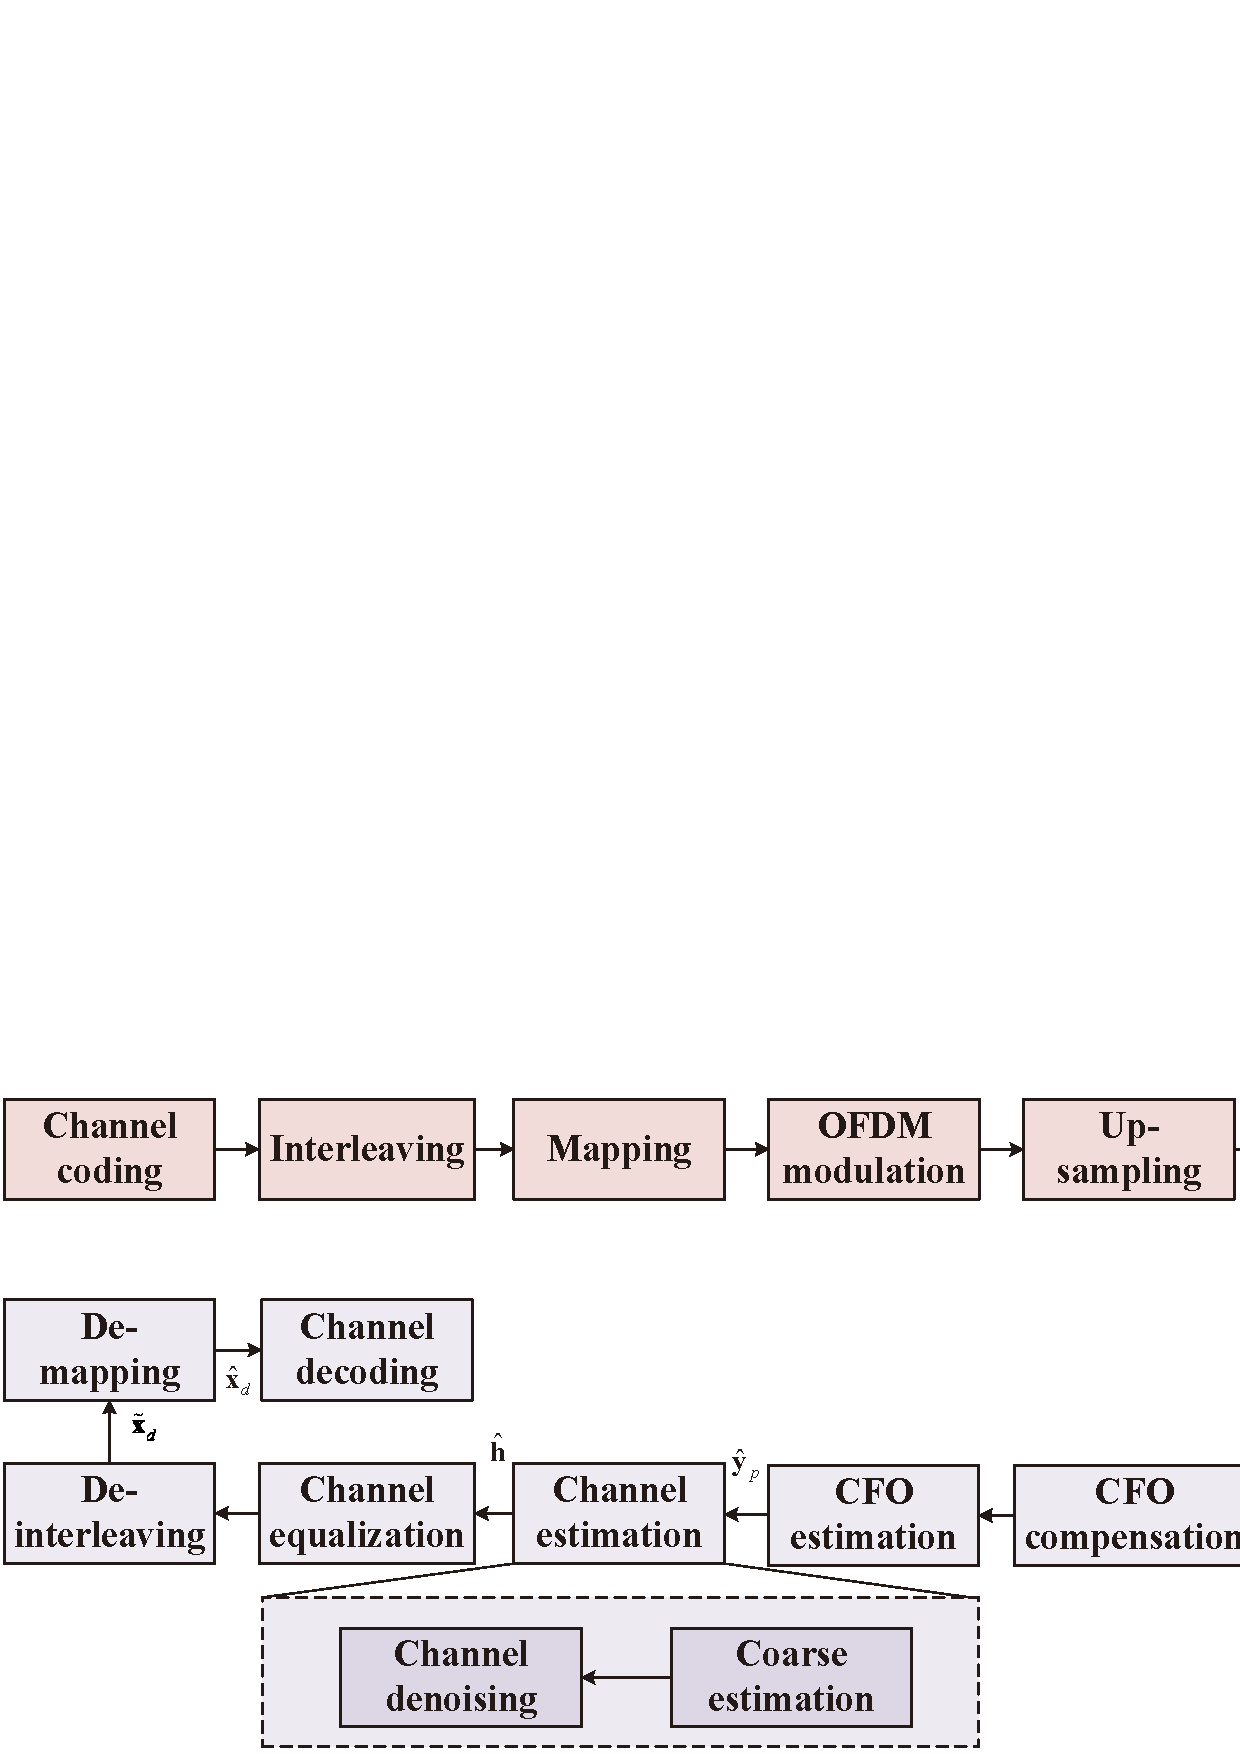
\includegraphics[width=\linewidth]{figs/flowchart.pdf}
	\caption{Flowchart of OFDM.}
	\label{fig:flowchart}
\end{figure}
\par Assuming that each OFDM symbol contains $K$ subcarriers, with the $k$-th subcarrier positioned at the frequency ${f_k} = k{f_\Delta }$, where $k = 0, 1, \cdots ,K-1$ and ${f_\Delta }$ denotes the frequency interval. The $K$ subcarriers are categorized into $K_a$ data subcarriers and $K_p$ pilot subcarriers, with their respective index sets denoted as $\mathcal{K}_a$ and $\mathcal{K}_p$ respectively. Hence, by performing a $K$-point IDFT, each OFDM baseband signal in the time domain ${\bf{x}}_t \in \mathbb{C}^{K \times 1}$ can be expressed as
\begin{eqnarray}\label{eq:x(n)}
	{\bf{x}}_t = {\bf{F}}_K^H{\bf{x}}_f\;.
\end{eqnarray}
Notation $\mathbf{x}_f \in \mathbb{C}^{K \times 1}$ denotes each mapped OFDM signal in the frequency domain, defined as $\mathbf{x}_f \triangleq {\left( {\mathbf{x}_f\left[ 0 \right],\mathbf{x}_f\left[ 1 \right], \cdots ,\mathbf{x}_f\left[ K-1 \right]} \right)^T}$. Subsequently, cyclic prefix (CP) insertion, up-sampling, pulse shaping, and carrier modulation are performed sequentially to generate the passband OFDM signal.
\par At the receiver, the wideband Doppler effect is compensated
by resampling, as noted in~\cite{li2008ofdm}, while the residual narrowband Doppler shift is modeled as CFO. The passband processing includes resampling, down-conversion, low-pass filtering, and CP removal. Assuming the CIR is time-invariant within one OFDM block and CP length $L_{cp}$ exceeds the maximum channel delay spread $L_h \le L_{cp}$, after down-conversion, low-pass filtering, and CP removal, the received baseband signal can be expressed as
\begin{equation}
	\label{eq:y_t}
	{{\bf{y}}_t} = {{\bf{\Gamma }} }_{\varepsilon}{{\bf{F}}^H}{{\bf{\Lambda }}}{{\bf{F}}_{L_h}}{\bf{h}} + {{\bf{w}}_t}\;,
\end{equation}
where ${{\bf{y}}_t} \triangleq {({y_t}\left[ 0 \right],{y_t}\left[ 1 \right], \cdots ,{y_t}\left[ {K - 1} \right])^T}$ represents the received time-domain vector. The matrix $\mathbf{\Gamma}_{\varepsilon} = \text{diag}(1, e^{j2\pi \varepsilon /K}, \dots, e^{j2\pi \varepsilon (K - 1)/K})$ denotes the CFO diagonal matrix characterized by the normalized frequency offset $\varepsilon$. Notation ${\bf{\Lambda }} = \text{diag}(\mathbf{x}_f)$ is the diagonal transmission matrix, and $\mathbf{F}_{L_h}$ denotes the submatrix formed by the first $L_h$ columns of the unitary DFT matrix $\mathbf{F}$. The vector ${\bf{h}} = {[ h[ 0 ], \cdots ,h[ {L_h - 1} ]]^T}$ represents the CIR, and $\mathbf{w}_t \sim \mathcal{CN}(\mathbf{0}, \sigma^2 \mathbf{I})$ denotes the additive Gaussian noise vector.
\par Assuming ${\bf{\Gamma }}_{\hat \varepsilon }^H \in \mathbb{C}^{K \times K}$ denotes the CFO compensation matrix with a estimated CFO value $ \hat \varepsilon $ and $\mathbf{P}_p$ denotes the pilot selection matrix, the compensated pilot signal in the frequency domain can be expressed as
\begin{eqnarray}\label{eq:y_p}
	{{\bf{y}}_p} &=& {{\bf{P}}_p}{{\bf{F}}}{\bf{\Gamma }}_\varepsilon ^H{\bf{y}}_t \nonumber \\
	&=& {{\bf{P}}_p}{{\bf{F}}}{\bf{\Gamma }}_{\hat \varepsilon} ^H{{\bf{\Gamma }}_{{\varepsilon }}}{\bf{F}}^H{{\bf{\Lambda }}}{{\bf{F}}_{{L_h}}}{\bf{h}} + {\bf{\Gamma }}_\varepsilon ^H{\bf{w}}\;,\\
	&=& {{\bf{P}}_p}{{\bf{F}}}{{\bf{\Gamma }}_{\Delta \varepsilon }}{\bf{F}}^H{{\bf{\Lambda }}}{{\bf{F}}_{{L_h}}}{\bf{h}} + {\bf{\Gamma }}_\varepsilon ^H{\bf{w}}_t \nonumber \\
	&=& {{\bf{\Phi }}_{\Delta \varepsilon }}{\bf{h}} + {{\bf{w}}_{p\varepsilon }} \nonumber \\
\end{eqnarray}
where
\begin{eqnarray}\label{eq:Phi_delta}
	{{\bf{\Phi }}_{\Delta \varepsilon }} = {{\bf{P}}_p}{\bf{F}}{{\bf{\Gamma }}_{\Delta \varepsilon }}{{\bf{F}}^H}{{\bf{\Lambda }}}{{\bf{F}}_{L_h}}\;,
\end{eqnarray}
\begin{eqnarray}\label{eq:Gamma_delta}
	{{\bf{\Gamma }}_{\Delta \varepsilon }} \buildrel \Delta \over = {\mathop{\rm diag}\nolimits} (1,{e^{j2\pi \Delta \varepsilon /K}}, \ldots ,{e^{j2\pi \Delta \varepsilon (K - 1)/K}})\;,
\end{eqnarray}
\begin{eqnarray}\label{eq:delta_varesilon}
  \Delta \varepsilon  = \varepsilon  - \hat \varepsilon \;.
\end{eqnarray}
Notations ${{\bf{\Phi }}_{\Delta \varepsilon }} \in \mathbb{C}^{K_p \times {L_h}}$ and ${{\bf{\Gamma }}_{\Delta \varepsilon }} \in \mathbb{C}^{K \times {K}}$ represents the distorted observation matrix and the residual phase rotation matrix respectively. Due to the residual CFO interference, the matrix product ${\bf{F}}{{\bf{\Gamma }}_{\Delta \varepsilon }}{{\bf{F}}^H}$ deviates from the identity matrix, with its energy becoming concentrated around the main diagonal. The channel estimation method, such as LS algorithm, is used to estimate the channel as
\begin{eqnarray}\label{eq:LS}
  {\bf{\hat h}} = {\left( {{\bf{\Phi }}_p^H{{\bf{\Phi }}_p}} \right)^{ - 1}}{\bf{\Phi }}_p^H{{\bf{y}}_p}\;,
\end{eqnarray}
where ${{\bf{\Phi }}_p} = {{\bf{\Lambda }}_p}{{\bf{F}}_{{L_h}}} \in \mathbb{C}^{K_p \times {L_h}}$ denotes the observation matrix and $\mathbf{\Lambda}_p$ denotes the diagonal transmission pilot matrix. Subsequently, channel equalization is applied to demodulation, such as the output OFDM symbols based on a linear equalizer can be expressed as
\begin{eqnarray}\label{eq:xbar}
	{{\bf{\hat x}}_f} = \frac{{{{\bf{y}}_a}}}{{{{\bf{F}}_a}{\bf{\hat h}}}}\;.
\end{eqnarray}
where $\mathbf{y}_a=\mathbf{P}_a \mathbf{y}$ denotes , and $\mathbf{F}_a$ denotes the submatrix formed by the data set index $\mathcal{K}_a$ rows of the matrix $\mathbf{F}_{L_h}$.
\par Note that, due to CFO residuals and channel estimation residuals, the noise no longer is pure Gaussian white noise as shown in~\eqref{eq:LS}. Since accurate UWA channel estimation is essential to equalization and system performance, and conventional channel denosing method lack of the utilization of the characteristic of UWA channels, this paper focuses on improving channel estimation accuracy through physics-inspired denoising.

%====================================================================
\section{Channel Model and Problem Formulation}
UWA propagation is characterized by severe complexity due to the dynamic nature of the underwater environment. Acoustic velocity gradients and medium inhomogeneities induce significant refraction and reflection, resulting in rich multipath propagation effects.

\subsection{Channel Decomposition Model} \label{sec:decomposition}
\par Based on physical propagation mechanisms, multipath components can be categorized into direct paths, sea surface reflections, and seafloor reflections, etc. Following the classification in~\cite{whitmarsh1963underwater}, these eigenpaths are decomposed into two distinct categories based on their temporal stability: static paths and dynamic paths.

\par Static paths originate from stable boundary interactions, including direct line-of-sight propagation, bottom reflections, and stable refracted paths. Since the water column structure, seafloor topography, and sound speed profile (SSP) remain relatively invariant over short observation intervals, static paths exhibit constant time delays and slowly varying amplitudes, manifesting strong temporal correlation. Conversely, dynamic paths are predominantly induced by the time-varying, non-specular sea surface driven by wind and waves. These components are characterized by rapid fluctuations in both delay and amplitude, resulting in weak temporal correlation. Fig.~\ref{fig:channel_mechanisms} illustrates these propagation mechanisms.

\begin{figure}[htbp]
	\centering
	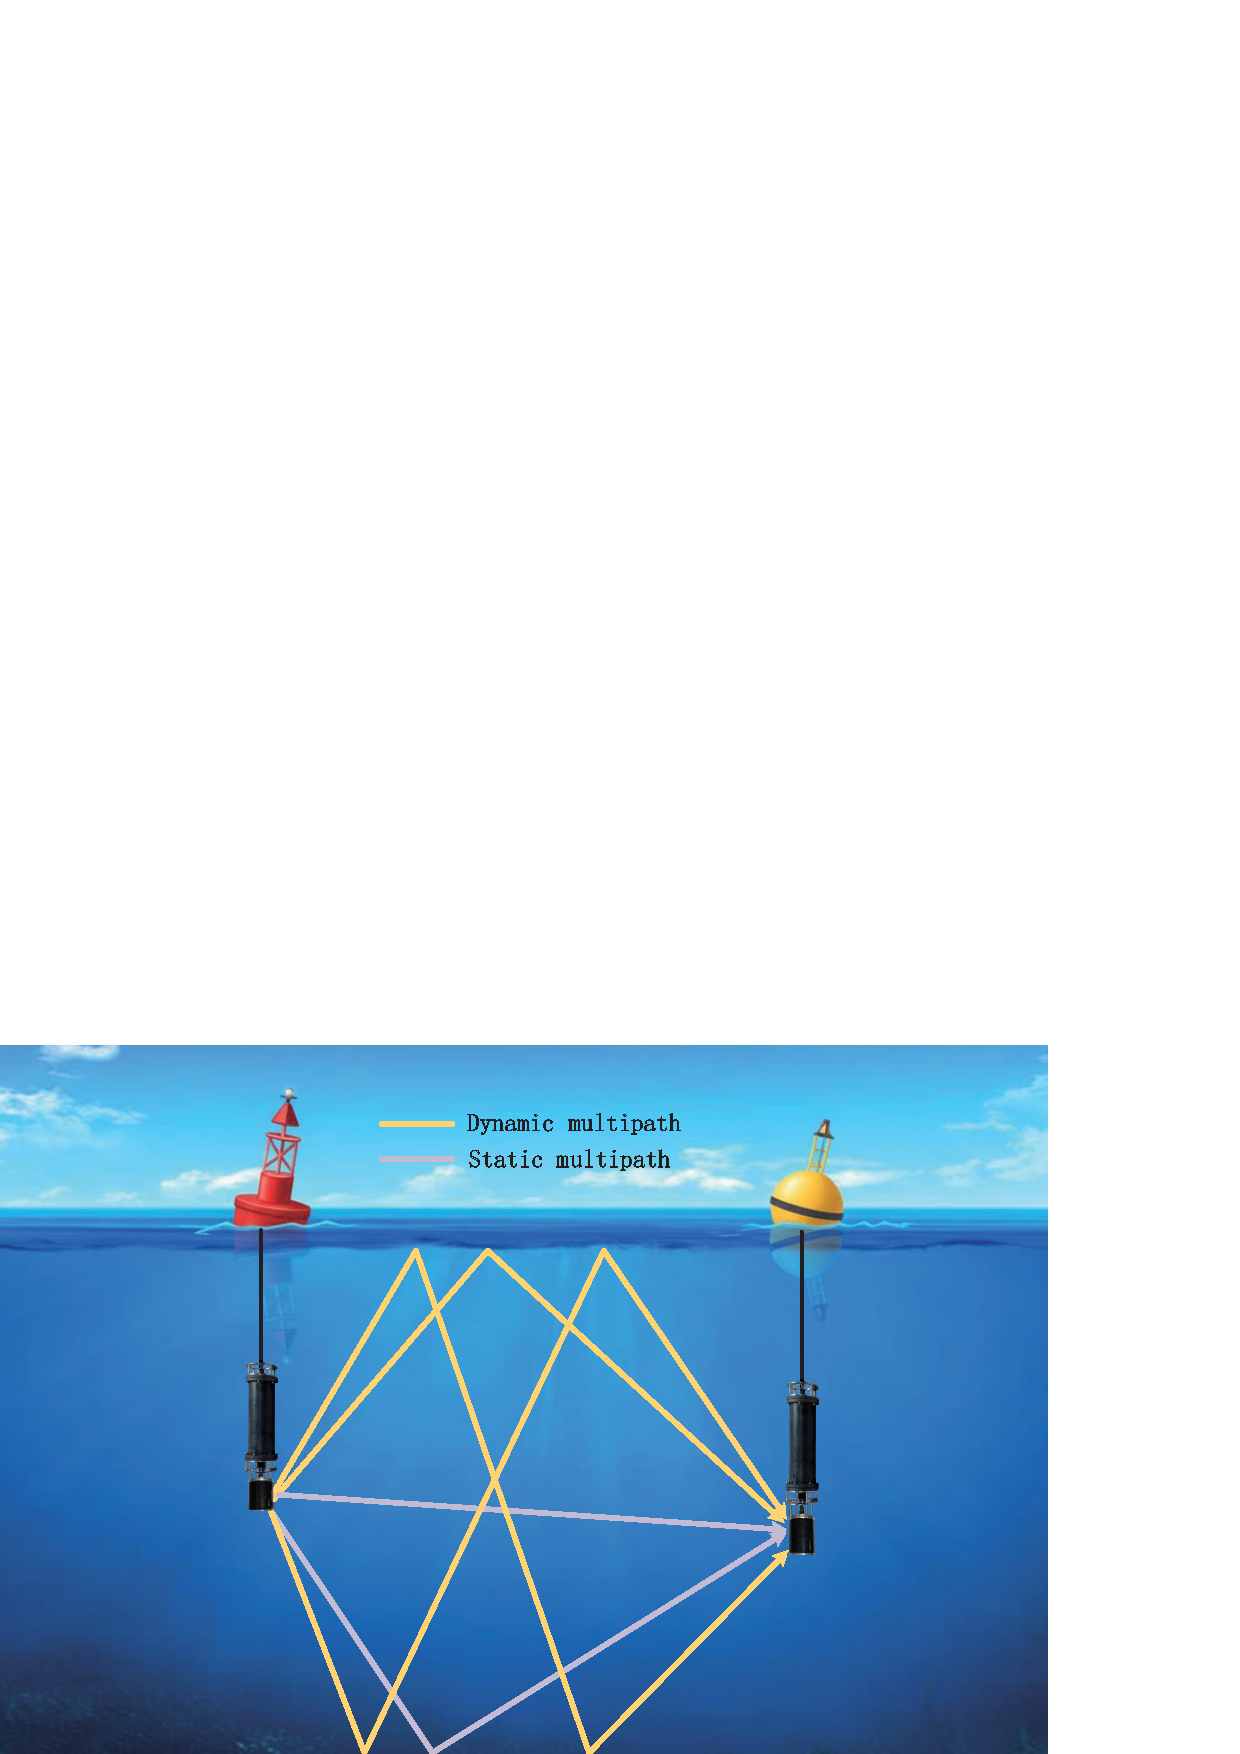
\includegraphics[width=\linewidth]{figs/channel_mechanisms.pdf}
	\caption{Schematic diagram of the channel propagation mechanisms illustrating static and dynamic multipath components.}
	\label{fig:channel_mechanisms}
\end{figure}

Mathematically, we model the UWA channel by decoupling these components. Let $N$ denote the channel delay spread length. The CIR vector at time slot $t$, denoted by $\mathbf{h}(t) \in \mathbb{C}^{N \times 1}$, is expressed as:
\begin{equation}\label{eq:h}
	\mathbf{h}(t) = \mathbf{h}_s(t) + \mathbf{h}_d(t),
\end{equation}
where $\mathbf{h}_s(t)$ and $\mathbf{h}_d(t)$ represent the static and dynamic channel vectors, respectively. Considering an observation window of $M$ consecutive time slots, the aggregate delay-time channel matrix $\mathbf{H} \in \mathbb{C}^{M \times N}$ is constructed by stacking the transposed CIR vectors:
\begin{equation}\label{eq:H}
	\mathbf{H} = \mathbf{H}_s + \mathbf{H}_d = 
	\begin{bmatrix}
		\mathbf{h}_s^T(t) \\
		\mathbf{h}_s^T(t+1) \\
		\vdots \\
		\mathbf{h}_s^T(t+M-1)
	\end{bmatrix} + 
	\begin{bmatrix}
		\mathbf{h}_d^T(t) \\
		\mathbf{h}_d^T(t+1) \\
		\vdots \\
		\mathbf{h}_d^T(t+M-1)
	\end{bmatrix}.
\end{equation}

\subsection{Physical Characteristics of Sub-channels} \label{sec:channel_characteristic}
In this subsection, we analyze the statistical properties of the decomposed channels in both the delay and time domains.

\subsubsection{Delay Domain}
UWA channels are inherently sparse. For a channel length $N$, the number of significant paths $\kappa$ satisfies $\kappa \ll N$, a property widely utilized in UWA channel denoising methods. Crucially, both the static and dynamic components inherit this sparsity property:
\begin{equation}
	\|\mathbf{h}_s(t)\|_0 = \kappa_s \ll N, \quad \|\mathbf{h}_d(t)\|_0 = \kappa_d \ll N,
\end{equation}
where $\kappa_s$ and $\kappa_d$ denote the sparsity levels of the static and dynamic sub-channels, respectively, with the total sparsity satisfying $\kappa \approx \kappa_s + \kappa_d$.

\subsubsection{Time Domain}
The two components exhibit distinct temporal statistics. Experimental studies~\cite{jiang2022exploiting, zhou2017exploiting} suggest that the amplitude of the static component typically follows a Ricean distribution (indicating a dominant stable component). In contrast, the dynamic component, particularly at large grazing angles, exhibits empirical statistics often fitted by a Gamma distribution, as shown in Fig.~\ref{fig:Gamma}.

\begin{figure}[htbp]
	\centering
	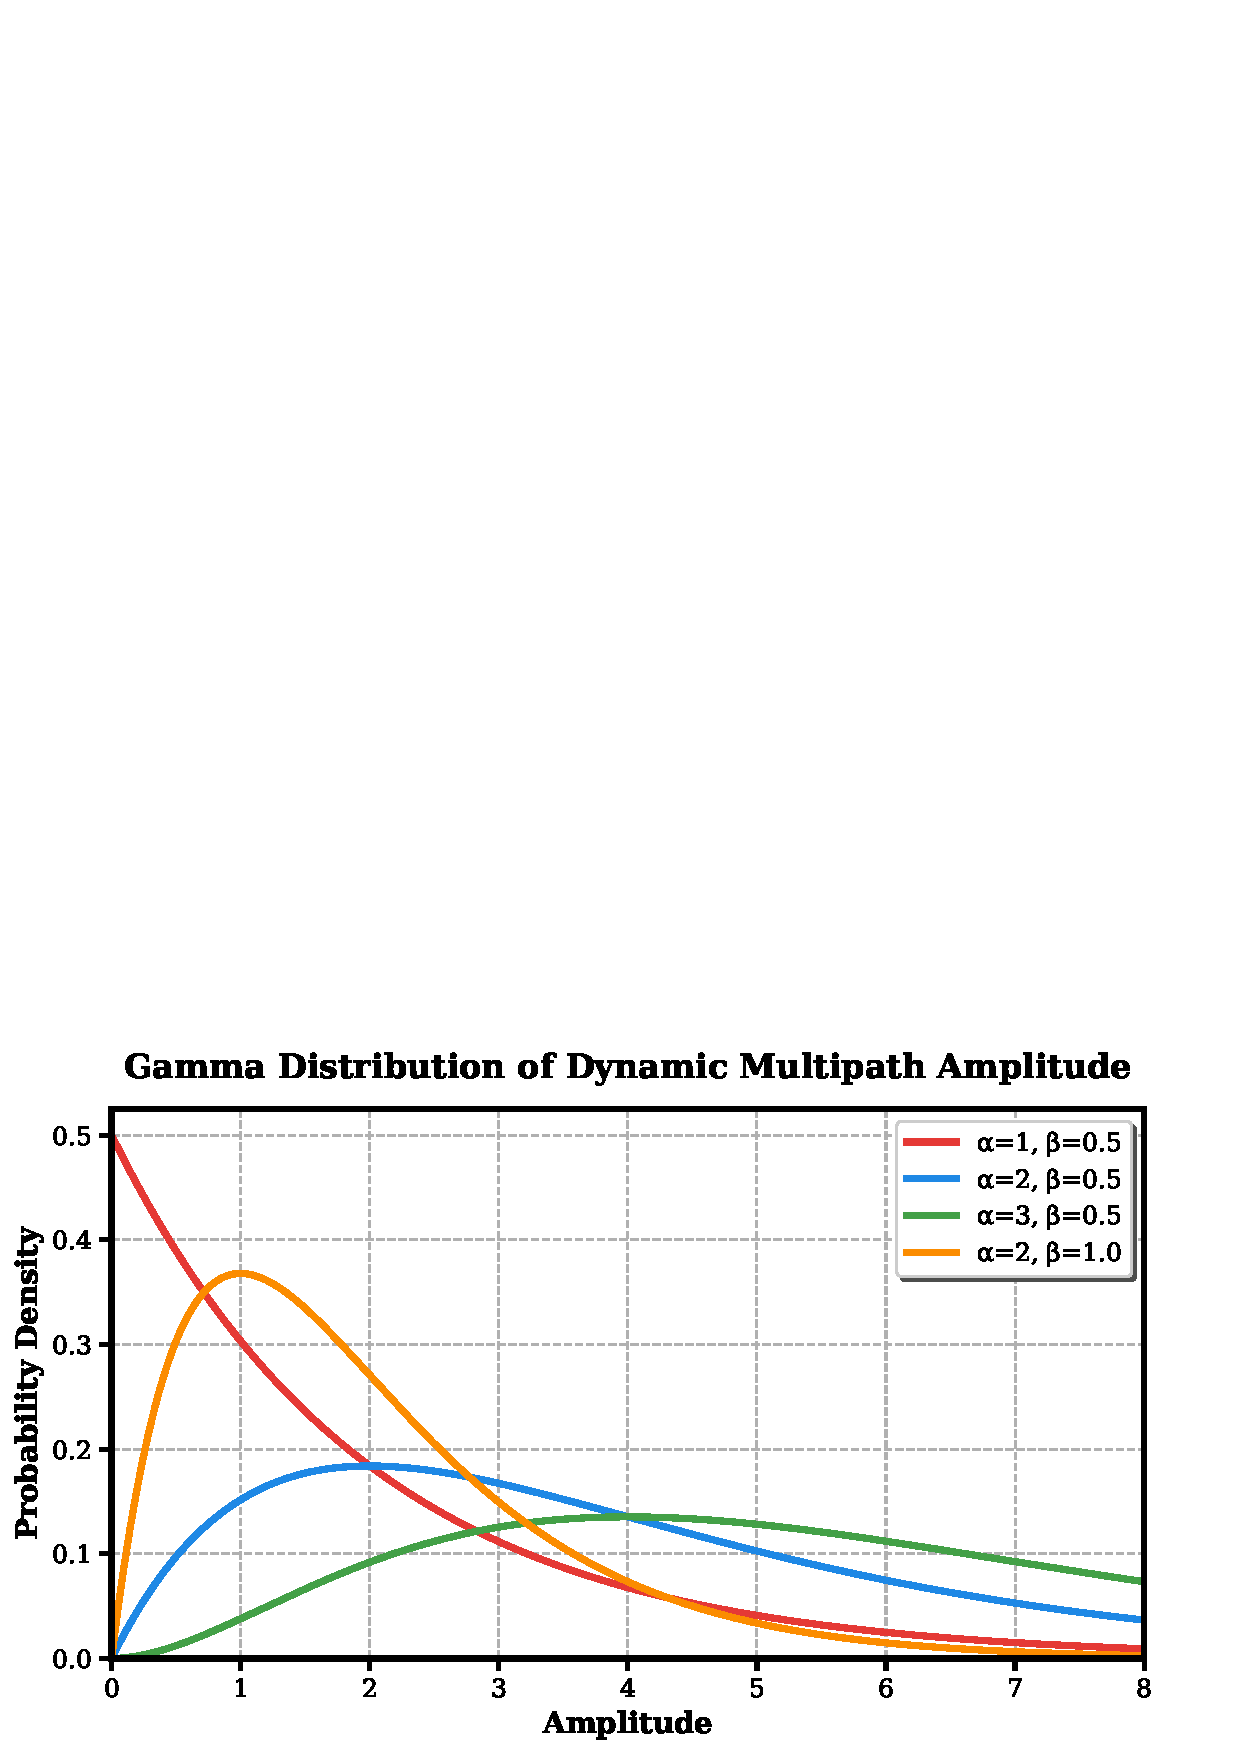
\includegraphics[width=\linewidth]{figs/Gamma.pdf}
	\caption{Probability density function of the dynamic multipath amplitude fitting a Gamma distribution.}
	\label{fig:Gamma}
\end{figure}

Specifically, let $h_{s,\tau}(t)$ denote the $\tau$-th tap of the static channel at time $t$. Its complex coefficient is modeled as a non-zero mean complex Gaussian variable:
\begin{equation}
	h_{s,\tau}(t) \sim \mathcal{CN}(\mu_s, \sigma_s^2).
\end{equation}
Due to environmental stability, the set of active tap indices for the static channel, denoted by $\Upsilon_s(t)$, remains invariant over the observation window:
\begin{equation}
	\Upsilon_s(t + 1) = \Upsilon_s(t).
\end{equation}

In contrast, the dynamic component $h_{d,\tau}(t)$ is modeled with a random phase and an amplitude $|h_{d,\tau}(t)|$ that follows a Gamma distribution:
\begin{equation}
	|h_{d,\tau}(t)| \sim \Gamma(\alpha_d, \beta_d),
\end{equation}
where $\alpha_d$ and $\beta_d$ are the shape and inverse scale parameters, respectively. Furthermore, the rapid motion of the sea surface introduces jitter in the path delays. This is modeled by adding a zero-mean random perturbation to the nominal path delays, with variance $\sigma_d^2$ quantifying the fluctuation intensity related to sea surface roughness~\cite{preisig2004surface}.

From the perspective of temporal correlation, the static component exhibits high coherence between adjacent time slots due to the stability of the water column and seafloor. This implies that the differential energy is negligible:
\begin{equation}
	\mathbb{E}\left[\|\mathbf{h}_s(t+\Delta t) - \mathbf{h}_s(t)\|_2^2\right] \approx 0,
\end{equation}
where $\Delta t$ is within the channel coherence time $T_c$. Conversely, the dynamic component decorrelates rapidly due to surface shake. The cross-correlation between adjacent time slots is weak:
\begin{equation} \label{eq:decorr}
	\mathbb{E}\left[\mathbf{h}_d^H(t + \Delta t)\mathbf{h}_d(t)\right] \approx 0, \quad \text{for } \Delta t \ge \tau_{\text{corr}},
\end{equation}
where $\tau_{\text{corr}}$ denotes the correlation time of the dynamic surface scattering.

\subsection{Problem Formulation}
Accurate CSI is critical for OFDM system performance but is often degraded by noise, including residual CFO interference, estimated channel error, and ambient noise. The goal is to recover the clean channel matrix $\mathbf{H}$ from noisy observations $\hat{\mathbf{H}}_{\text{raw}}$. The baseline denoising problem minimizes the mean squared error (MSE):
\begin{equation}
	\min_{\hat{\mathbf{H}}} \mathbb{E} \left[ \|\mathbf{H} - \hat{\mathbf{H}}\|_F^2 \right].
\end{equation}
Conventional methods treat $\mathbf{H}$ as a homogeneous entity. In this paper, leveraging the physics-based decomposition analyzed above, we reformulate the problem to jointly estimate the static and dynamic components by exploiting their distinct structures. The optimization problem is formulated as:
\begin{equation} \label{eq:optimization}
	\begin{aligned}
		& \min_{\hat{\mathbf{H}}_s, \hat{\mathbf{H}}_d} \mathbb{E} \left[ \underbrace{\|\mathbf{H}_s - \hat{\mathbf{H}}_s\|_F^2}_{\text{Static Fidelity}} + \underbrace{\|\mathbf{H}_d - \hat{\mathbf{H}}_d\|_F^2}_{\text{Dynamic Fidelity}} \right] \\
		& \text{subject to:} \quad \hat{\mathbf{H}}_s \in \mathcal{S}, \quad \hat{\mathbf{H}}_d \in \mathcal{D},
	\end{aligned}
\end{equation}
where $\mathcal{S}$ represents the set of matrices satisfying sparsity and temporal consistency constraints (reflecting the stable sparse support), and $\mathcal{D}$ represents the set of matrices satisfying specific low-rank or structural constraints consistent with dynamic scattering. The final estimated channel is reconstructed as $\hat{\mathbf{H}} = \hat{\mathbf{H}}_s + \hat{\mathbf{H}}_d$.

This decomposition problem is ill-posed without strong priors. While classical methods struggle with unknown sparsity levels or rank deficiency, the proposed physics-inspired deep learning framework (detailed in the subsequent section) learns these implicit constraints from data.

% =========================================================================
\section{Theoretical Foundations}
\par Before describing DSS-Net, we establish theoretical connections to sparse recovery and low-rank matrix completion that motivate our physics-informed loss function design.

\subsection{Sparse Recovery Framework}
\par Consider the Delay-Doppler domain representation of static component via $M\times M$ DFT matrix $\mathbf{F}_M$
\begin{equation}
	{{\bf{X}}_s} = {\bf{F}}_M{{\bf{H}}_s}\;,
\end{equation}
where $\mathbf{X}_{\mathrm{s}}$ is approximately $k$-sparse with $k \ll MN$. The observation model becomes
\begin{equation}
\widetilde{\mathbf{H}}=\mathbf{F}_M^H\mathbf{X}_{\mathrm{s}}+\mathbf{H}_{\mathrm{d}}+\mathbf{N}\;,
\end{equation}
where $\mathbf{N}$ denotes background noise. If the sensing operator $\mathcal{A}(\mathbf{X})=\mathbf{F}_M^H\mathbf{X}$ satisfies restricted isometry property (RIP) of order $2k$ with constant $\delta_{2k}<\sqrt{2}-1$ \cite{Candes2005Decoding}, then $\ell_1$ minimization
\begin{equation}
\min_{\mathbf{X}}\|\mathbf{X}\|_1\quad\text{s.t.}\quad\|\widetilde{\mathbf{H}}-\mathbf{F}_M^H\mathbf{X}-\mathbf{H}_{\mathrm{d}}\|_F\leq\epsilon
\end{equation}
recovers $\mathbf{X}_{\mathrm{s}}$ with error $\|\mathbf{X}_{\mathrm{s}}-\hat{\mathbf{X}}_{\mathrm{s}}\|_F\leq C\sigma_n\sqrt{k\log(MN)}$ for constant $C$ depending on $\delta_{2k}$ \cite{Candes2006Stable}.

\par The $\ell_1$ term in our loss function serves as a convex relaxation of the sparsity constraint, enabling stable recovery under noise.

\subsection{Low-Rank Matrix Recovery}

For dynamic component with rank $r \ll \min(M,N)$, consider the nuclear norm minimization:
\begin{equation}
\min_{\mathbf{X}}\|\mathbf{X}\|_*\quad\text{s.t.}\quad\|\widetilde{\mathbf{H}}-\mathbf{H}_{{s}}-\mathbf{X}\|_F\leq\epsilon,
\end{equation}
where $\|\mathbf{X}\|_*=\sum_i\sigma_i(\mathbf{X})$ is the sum of singular values. Under incoherence conditions \cite{Candes2009Exact}, this recovers $\mathbf{H}_{{d}}$ exactly when number of observations exceeds $O(r(M+N)\log^2(MN))$.

The nuclear norm gradient has a simple form \cite{Watson1992Characterization}:
\begin{equation}
\nabla_{\mathbf{X}}\|\mathbf{X}\|_*=\mathbf{U}\mathbf{V}^H,
\end{equation}
where $\mathbf{X}=\mathbf{U}\mathbf{\Sigma}\mathbf{V}^H$ is the SVD, enabling efficient back propagation in our network.

\subsection{Separation via Orthogonality}

To ensure unique decomposition, we enforce low correlation between static and dynamic components. Define correlation:
\begin{equation}
\rho(\mathbf{H}_{\mathrm{s}},\mathbf{H}_{\mathrm{d}})=\frac{|\langle\mathbf{H}_{\mathrm{s}},\mathbf{H}_{\mathrm{d}}\rangle_F|}{\|\mathbf{H}_{\mathrm{s}}\|_F\|\mathbf{H}_{\mathrm{d}}\|_F},
\end{equation}
where $\langle\mathbf{A},\mathbf{B}\rangle_F=\text{tr}(\mathbf{A}^H\mathbf{B})$ is Frobenius inner product. Minimizing $\rho$ encourages near-orthogonal decomposition, reducing ambiguity.

\textit{Proposition 1:} If $\mathbf{H}_{\mathrm{s}}$ is $k$-sparse in angular domain and $\mathbf{H}_{\mathrm{d}}$ has rank $r$ with incoherent singular vectors, then $\rho(\mathbf{H}_{\mathrm{s}},\mathbf{H}_{\mathrm{d}})\leq\sqrt{kr/MN}$ with high probability under random scatterer distribution.

\par This result justifies our separation quality loss, which minimizes correlation between estimated components. The proof is provided in Appendix~A.

% =========================================================================
\section{DSS-Net Architecture}
\par The DSS-Net is included into the receiver of UWA communication systems, as shown in the upper part of Fig.~\ref{fig:DSS-Net}. The DSS-Net is focusing on optimize the output estimated channel, which improving the equalization performance.

\begin{figure*}[htbp]
	\centering
	\includegraphics[width=\textwidth]{figs/dss_net_framework.pdf}
	\caption{Overview of the proposed DSS-Net architecture. The framework consists of three stages: (a) Preprocessing: the complex channel matrix is decomposed into real and imaginary components; (b) DSS-Net: a shared encoder extracts common features, while dual symmetric decoders separately reconstruct static and dynamic components with squeeze-and-excitation (SE) attention at the bottleneck; (c) Postprocessing: the outputs are combined to obtain the denoised channel.}
	\label{fig:DSS-Net}
\end{figure*}

\subsection{Network Overview}
\par DSS-Net adopts a U-Net encoder-decoder architecture~\cite{Ronneberger2015UNet} with three key innovations: (i) shared encoder extracting common features; (ii) dual symmetric decoders for parallel reconstruction; (iii) squeeze-and-excitation (SE) attention at the bottleneck~\cite{Hu2018SqueezeExcitation}. The architecture is illustrated in Fig.~\ref{fig:DSS-Net}.

\par \textit{Input Representation:} The complex channel $\widetilde{\mathbf{H}}\in\mathbb{C}^{M\times N}$ is decomposed into real and imaginary parts:
\begin{equation}
\mathbf{X}_{\text{in}}=[\Re(\widetilde{\mathbf{H}});\Im(\widetilde{\mathbf{H}})]\in\mathbb{R}^{2\times M\times N}.
\end{equation}

\par \textit{Encoder:} Four downsampling blocks with channel dimensions $64\to128\to256\to512\to512$. Each block contains:
\begin{equation}
\begin{aligned}
\bm{z}_1&=\text{BN}(\text{LeakyReLU}(\text{Conv}_{3\times 3}(\bm{x}))),\\
\bm{z}_2&=\text{BN}(\text{LeakyReLU}(\text{Conv}_{3\times 3}(\bm{z}_1))),\\
\bm{x}_{\text{down}}&=\text{MaxPool}_{2\times 2}(\bm{z}_2).
\end{aligned}
\end{equation}
Skip connections preserve $\{\bm{z}_2^{(i)}\}_{i=1}^4$ for decoder reconstruction.

\par \textit{Attention Bottleneck:} At the deepest layer, the SE module computes channel-wise attention:
\begin{equation}
\begin{aligned}
\bm{s}&=\text{GAP}(\bm{z}_{\text{bottleneck}})\in\mathbb{R}^{512},\\
\bm{w}&=\sigma(\bm{W}_2\delta(\bm{W}_1\bm{s}+\bm{b}_1)+\bm{b}_2),\\
\bm{z}_{\text{attn}}&=\bm{z}_{\text{bottleneck}}\odot\bm{w},
\end{aligned}
\end{equation}
where GAP is global average pooling, $\delta$ is ReLU, $\sigma$ is sigmoid, $\bm{W}_1\in\mathbb{R}^{64\times512}$, $\bm{W}_2\in\mathbb{R}^{512\times64}$ (reduction ratio 8).

\par \textit{Decoders:} Two structurally identical decoders with upsampling:
\begin{equation}
\begin{aligned}
\bm{z}_{\text{up}}&=\text{ConvTranspose}_{2\times 2}(\bm{z}),\\
\bm{z}_{\text{cat}}&=[\bm{z}_{\text{up}};\bm{z}_{\text{skip}}],\\
\bm{z}_{\text{out}}&=\text{DoubleConv}(\bm{z}_{\text{cat}}).
\end{aligned}
\end{equation}
Final outputs are two-channel maps converted to complex:
\begin{equation}
\hat{\bm{H}}_{\mathrm{s}}=\bm{Y}_{\mathrm{s}}^{(1)}+j\bm{Y}_{\mathrm{s}}^{(2)},\quad\hat{\bm{H}}_{\mathrm{d}}=\bm{Y}_{\mathrm{d}}^{(1)}+j\bm{Y}_{\mathrm{d}}^{(2)}.
\end{equation}

\subsection{Design Rationale}

\par \textit{Parameter Sharing:} The shared encoder reduces parameters compared to two independent encoders while learning common low-level features.

\par \textit{Symmetric Decoders:} Our symmetric design (43.6M parameters vs. 62M for dual full networks) avoids bias toward either component and achieves 42\% parameter reduction.

\par \textit{Attention Mechanism:} The SE module enables adaptive feature selection, emphasizing informative frequency bands for static-dynamic separation.

\subsection{Computational Complexity}

\par Per-sample complexity is dominated by convolutions:
\begin{equation}
\mathcal{C}=\sum_{l=1}^{L}K_l^2C_{\text{in}}^{(l)}C_{\text{out}}^{(l)}H_lW_l,
\end{equation}
where $K_l$ is kernel size, $C$ are channels, $H_l,W_l$ are spatial dimensions at layer $l$. For our architecture with $M=100,N=150$:
\begin{equation}
\mathcal{C}\approx9\times64^2\times100\times150\approx5.5\text{ GFLOPs}.
\end{equation}
This enables real-time processing at $>$180 FPS on NVIDIA A100 GPU.

% =========================================================================
\section{Physics-Informed Loss Function}

\par We design a multi-term objective function embedding domain knowledge from UWA channel physics.

\subsection{Weighted Reconstruction Loss}

\par The primary objective ensures fidelity to ground truth:
\begin{multline}
\mathcal{L}_{\text{recon}}=\frac{1}{B}\sum_{b=1}^{B}\Bigl[\alpha_{\mathrm{s}}\|\hat{\mathbf{H}}_{\mathrm{s}}^{(b)}-\mathbf{H}_{\mathrm{s}}^{(b)}\|_F^2\\
+\alpha_{\mathrm{d}}\|\hat{\mathbf{H}}_{\mathrm{d}}^{(b)}-\mathbf{H}_{\mathrm{d}}^{(b)}\|_F^2+\alpha_{\mathrm{t}}\|\hat{\mathbf{H}}^{(b)}-\mathbf{H}^{(b)}\|_F^2\Bigr],
\end{multline}
where $\hat{\mathbf{H}}=\hat{\mathbf{H}}_{\mathrm{s}}+\hat{\mathbf{H}}_{\mathrm{d}}$. We set $\alpha_{\mathrm{s}}=1$, $\alpha_{\mathrm{d}}=2$, $\alpha_{\mathrm{t}}=3$ to prioritize total channel accuracy while ensuring component-level supervision.

The hierarchy $\alpha_{\mathrm{t}}>\alpha_{\mathrm{d}}>\alpha_{\mathrm{s}}$ reflects that: (i) end-to-end performance depends on total channel; (ii) dynamic component is harder to estimate due to rapid variation; (iii) static component is easier given its smoothness.

\subsection{Sparsity-Promoting Regularization}

\par To encourage sparse static component:
\begin{equation}
\mathcal{L}_{\text{sparse}}=\frac{1}{B}\sum_{b=1}^{B}\|\hat{\mathbf{H}}_{\mathrm{s}}^{(b)}\|_1=\frac{1}{B}\sum_{b=1}^{B}\sum_{m,n}|\hat{H}_{\mathrm{s},mn}^{(b)}|.
\end{equation}

According to sparse recovery theory \cite{Candes2005Decoding}, $\ell_1$ can minimization provably recovers sparse signals under RIP. Our weak regularization ($\lambda_{\text{sparse}}=10^{-4}$) provides soft constraint without over-constraining.

\subsection{Nuclear Norm Regularization}

\par To promote low-rank dynamic component:
\begin{equation}
\mathcal{L}_{\text{rank}}=\frac{1}{B}\sum_{b=1}^{B}\|\hat{\mathbf{H}}_{\mathrm{d}}^{(b)}\|_*=\frac{1}{B}\sum_{b=1}^{B}\sum_{i=1}^{\min(M,N)}\sigma_i(\hat{\mathbf{H}}_{\mathrm{d}}^{(b)}),
\end{equation}
where $\sigma_i$ are singular values. Nuclear norm is tightest convex relaxation of matrix rank \cite{Recht2010Guaranteed}.

Implementation: We compute SVD in float32 for numerical stability:
\begin{equation}
\hat{\mathbf{H}}_{\mathrm{d}}^{\text{fp32}}=\mathbf{U}\mathbf{\Sigma}\mathbf{V}^H,\quad\nabla_{\hat{\mathbf{H}}_{\mathrm{d}}}\|\hat{\mathbf{H}}_{\mathrm{d}}\|_*=\mathbf{U}\mathbf{V}^H.
\end{equation}

\subsection{Temporal Correlation Loss}

\par We exploit different temporal characteristics of static and dynamic components.

\par \textit{Static Smoothness:} Penalize large temporal variations:
\begin{equation}
\mathcal{L}_{\text{temp}}^s=\frac{1}{B}\sum_{b=1}^{B}\sum_{i}\|[\hat{\mathbf{H}}_{\mathrm{s}}^{(b)}]_{:,i+1}-[\hat{\mathbf{H}}_{\mathrm{s}}^{(b)}]_{:,i}\|_2^2,
\end{equation}
where the subscript $:,i$ denotes $i$-th column (frequency or spatial dimension).

\par \textit{Dynamic Variation:} Encourage moderate change via hinge loss:
\begin{equation}
\mathcal{L}_{\text{temp}}^d=\frac{1}{B}\sum_{b=1}^{B}\max\Bigl(0,\epsilon-\sum_{i}\|[\hat{\mathbf{H}}_{\mathrm{d}}^{(b)}]_{:,i+1}-[\hat{\mathbf{H}}_{\mathrm{d}}^{(b)}]_{:,i}\|_2^2\Bigr),
\end{equation}
with threshold $\epsilon=0.01$. This prevents the degenerate solution $\hat{\mathbf{H}}_{\mathrm{d}}\approx 0$.

Total temporal loss: $\mathcal{L}_{\text{temp}}=\mathcal{L}_{\text{temp}}^s+\mathcal{L}_{\text{temp}}^d$.

\subsection{Separation Quality Metric}

\par To avoid degenerate solutions where both decoders output similar matrices, we minimize correlation:
\begin{equation}
\mathcal{L}_{\text{sep}}=-\frac{1}{B}\sum_{b=1}^{B}\rho(\hat{\mathbf{H}}_{\mathrm{s}}^{(b)},\hat{\mathbf{H}}_{\mathrm{d}}^{(b)}),
\end{equation}
where Pearson correlation is
\begin{equation}
\rho(\mathbf{A},\mathbf{B})=\frac{\langle\mathbf{A}-\bar{\mathbf{A}},\mathbf{B}-\bar{\mathbf{B}}\rangle_F}{\|\mathbf{A}-\bar{\mathbf{A}}\|_F\|\mathbf{B}-\bar{\mathbf{B}}\|_F},
\end{equation}
with $\bar{\mathbf{A}}=\frac{1}{MN}\sum_{mn}A_{mn}$ being mean. Negative sign ensures lower correlation yields smaller loss.

\subsection{Total Objective}

\par Combining all terms:
\begin{equation}
\begin{aligned}
\mathcal{L}_{\text{total}}=&\mathcal{L}_{\text{recon}}+\lambda_{\text{sparse}}\mathcal{L}_{\text{sparse}}+\lambda_{\text{rank}}\mathcal{L}_{\text{rank}}\\
&+\lambda_{\text{temp}}\mathcal{L}_{\text{temp}}+\lambda_{\text{sep}}\mathcal{L}_{\text{sep}},
\end{aligned}
\end{equation}
with hyperparameters $\lambda_{\text{sparse}}=\lambda_{\text{rank}}=10^{-4}$, $\lambda_{\text{temp}}=10^{-2}$, $\lambda_{\text{sep}}=5\times10^{-2}$ tuned via validation.

\par In contrast, standard single-decoder U-Net uses only $\mathcal{L}_{\text{MSE}}=\|\hat{\mathbf{H}}-\mathbf{H}\|_F^2$, without physics-informed guidance from decomposition structure, sparsity/low-rank priors, and temporal correlation.

% =========================================================================
%\section{Dataset and Implementation}
\section{Simulation Experiments}
\par We evaluate DSS-Net against baseline methods including no processing, SVD truncation~\cite{suresh2017two}, Wavelet Shrinkage~\cite{Donoho1995Wavelet}, CResNet~\cite{CResNet_TWC21}, DnCNN~\cite{Zhang2017DnCNN}, and U-Net~\cite{wei2021physics}. Performance is evaluated using normalized mean squared error (NMSE) and bit error rate (BER). The NMSE is defined as follows:
\begin{equation}
	\text{NMSE}_{\text{dB}}=10\log_{10}\frac{\|\mathbf{H}-\hat{\mathbf{H}}\|_F^2}{\|\mathbf{H}\|_F^2}\;.
\end{equation}
\subsection{Ray-Tracing Channel Generation}
\par We use the Bellhop ray-tracing model~\cite{bellhop} to generate UWA CIR. The channel matrix is constructed following the decomposition model in Section~\ref{sec:decomposition}. Table~\ref{tab:Bellhop} lists the simulation parameters. Transmitter and receiver depths range from 0.5~m to 13.5~m in 15~m water depth, with horizontal distances from 0.5~km to 5~km. The SSP, shown in Fig.~\ref{fig:S_SSP}, is derived from sea trial measurements in Xiamen Harbor.
\begin{table}[!htbp]
	\caption{\textsc{Ray-Tracing Dataset Generation Parameters.} Channel impulse responses are generated using the Bellhop acoustic ray-tracing model with the sound speed profile measured in Xiamen Harbor. Static and dynamic multipath components are distinguished by reflection counts from sea floor and sea surface, respectively.}
	\label{tab:Bellhop}
	\centering
	\setlength{\tabcolsep}{4pt}
	\renewcommand\arraystretch{1.15}
	\small
	\begin{tabular}{p{150pt} >{\centering\arraybackslash}p{25pt} >{\centering\arraybackslash}p{50pt}}
		\toprule[1.5pt]
		\rowcolor{tableheader}
		\textbf{Parameter} & \textbf{Symbol} & \textbf{Value}\\
		\midrule[1pt]
		\rowcolor{tablerow1}
		Depth of transmitter (m)	&$L_{T}$	& 0.5 -- 13.5 \\
		\rowcolor{tablerow2}
		Depth of receiver (m)		&$L_{R}$	& 0.5 -- 13.5 \\
		\rowcolor{tablerow1}
		Depth of water (m)			&$L_W$	& 15 \\
		\rowcolor{tablerow2}
		Horizontal distances (km)	&$L_0$	& 0.5 -- 5 \\
		\midrule[0.5pt]
		\rowcolor{tablerow1}
		Mean of static amplitude	&$\mu_s$	& 0	\\
		\rowcolor{tablerow2}
		Variance of static amplitude	&$\sigma_s^2$			& 0.1 \\
		\midrule[0.5pt]
		\rowcolor{tablerow1}
		Gamma shape (dynamic)  &$\alpha_d$	& 0.5	\\
		\rowcolor{tablerow2}
		Gamma inverse scale (dynamic) &$\beta_d$	& 0.3	\\
		\rowcolor{tablerow1}
		Mean of dynamic delay &$\mu_d$					& 0	\\
		\rowcolor{tablerow2}
		Variance of dynamic delay				&$\sigma_d^2$			& 0.4 \\
		\bottomrule[1.5pt]
	\end{tabular}
	\renewcommand\arraystretch{1.0}
\end{table}

\par To generate the channel matrix from the CIRs generated by the Bellhop model, we adopt the decomposition model and characteristics analyzed in Section~\ref{sec:decomposition}. The relevant parameters are also summarized in Table~\ref{tab:Bellhop}. The static and dynamic multipath determination depends on the output reflection counts caused by sea floor and sea surface in the Bellhop model. A sample of channel matrix and its decomposition is shown in Fig.~\ref{fig:matrix}, showing the characteristic of static and dynamic in the time domain. This yields supervised triplets $(\mathbf{H}_s,\mathbf{H}_d,\mathbf{H})$ for training.

\begin{figure}[!htbp]
	\centering
	\subfloat[\label{fig:S_SSP}]
{
	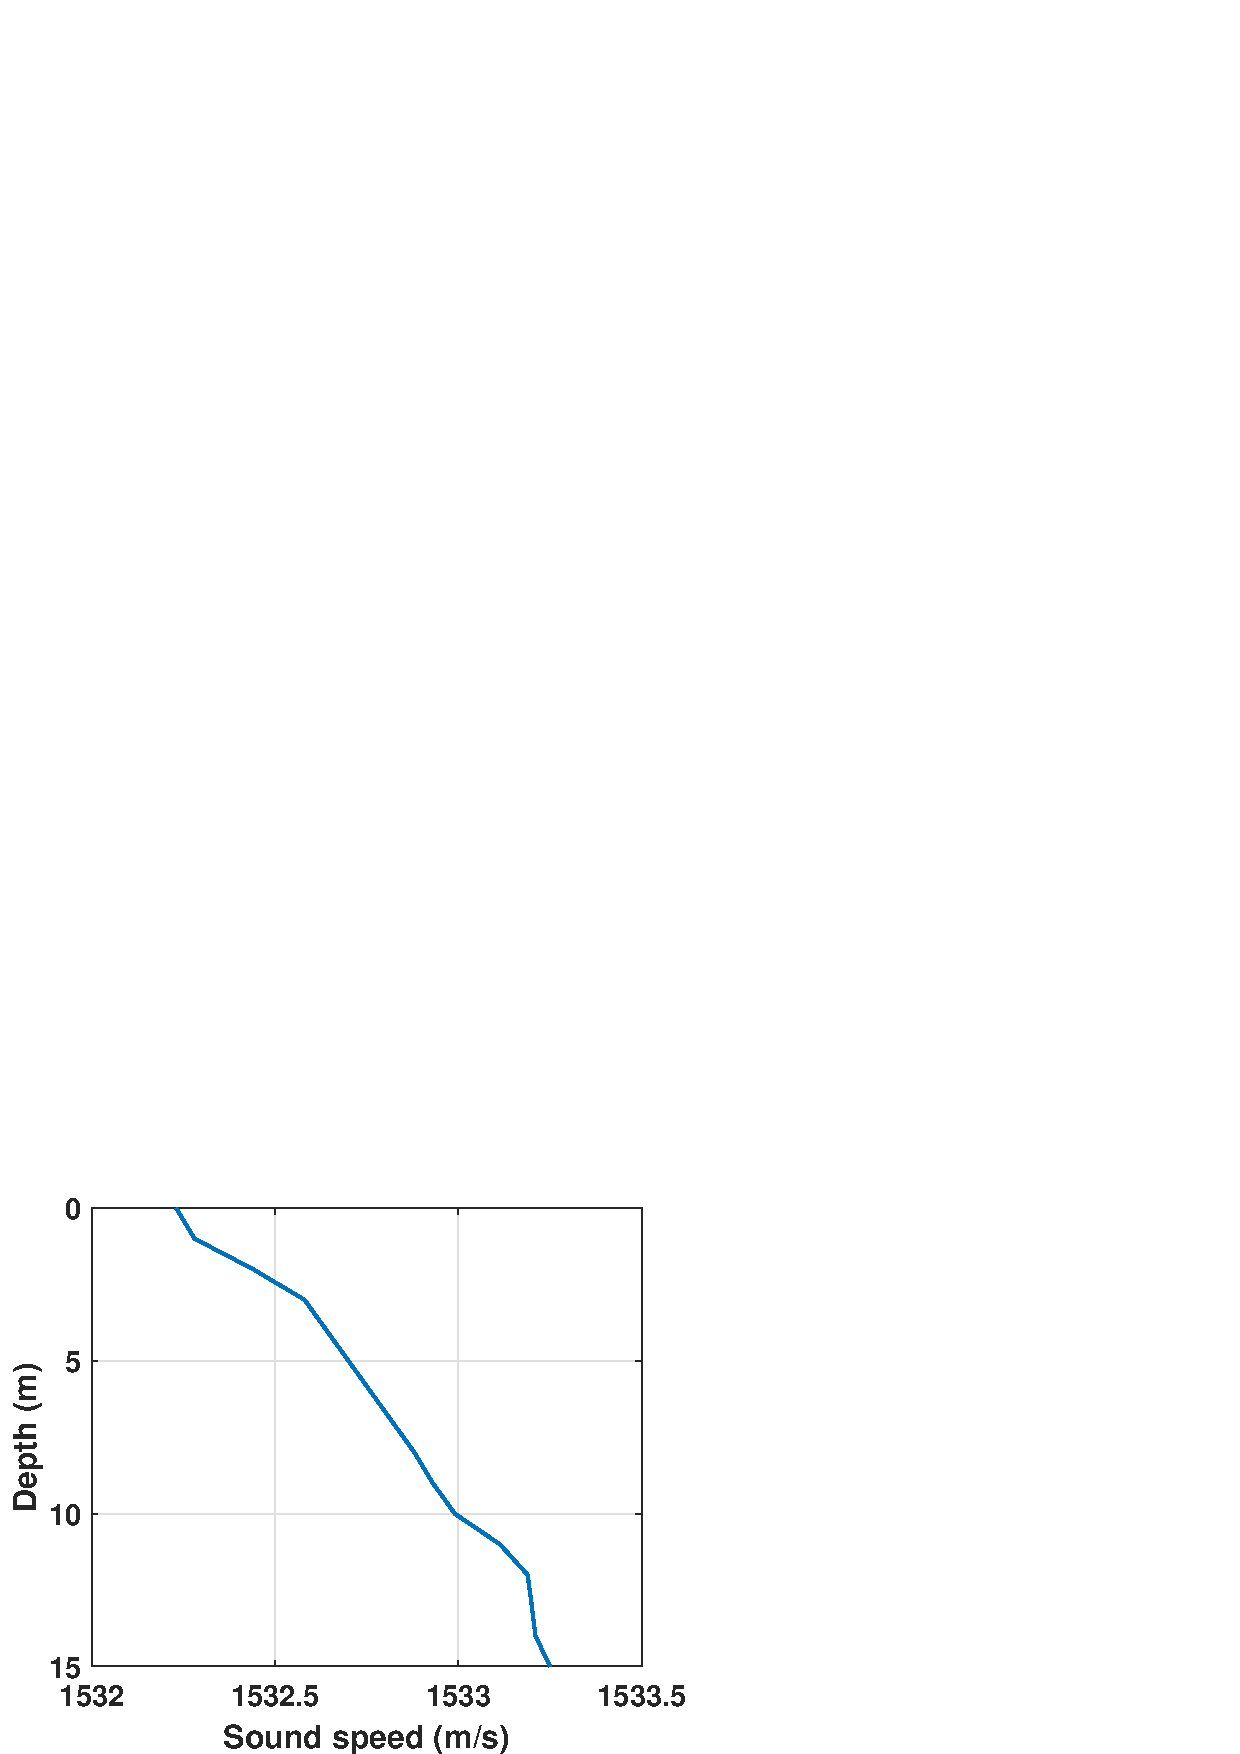
\includegraphics[width=0.45\linewidth]{figs/Bellhop_SSP.pdf}
}
	\subfloat[\label{fig:All_channel}]
	{
		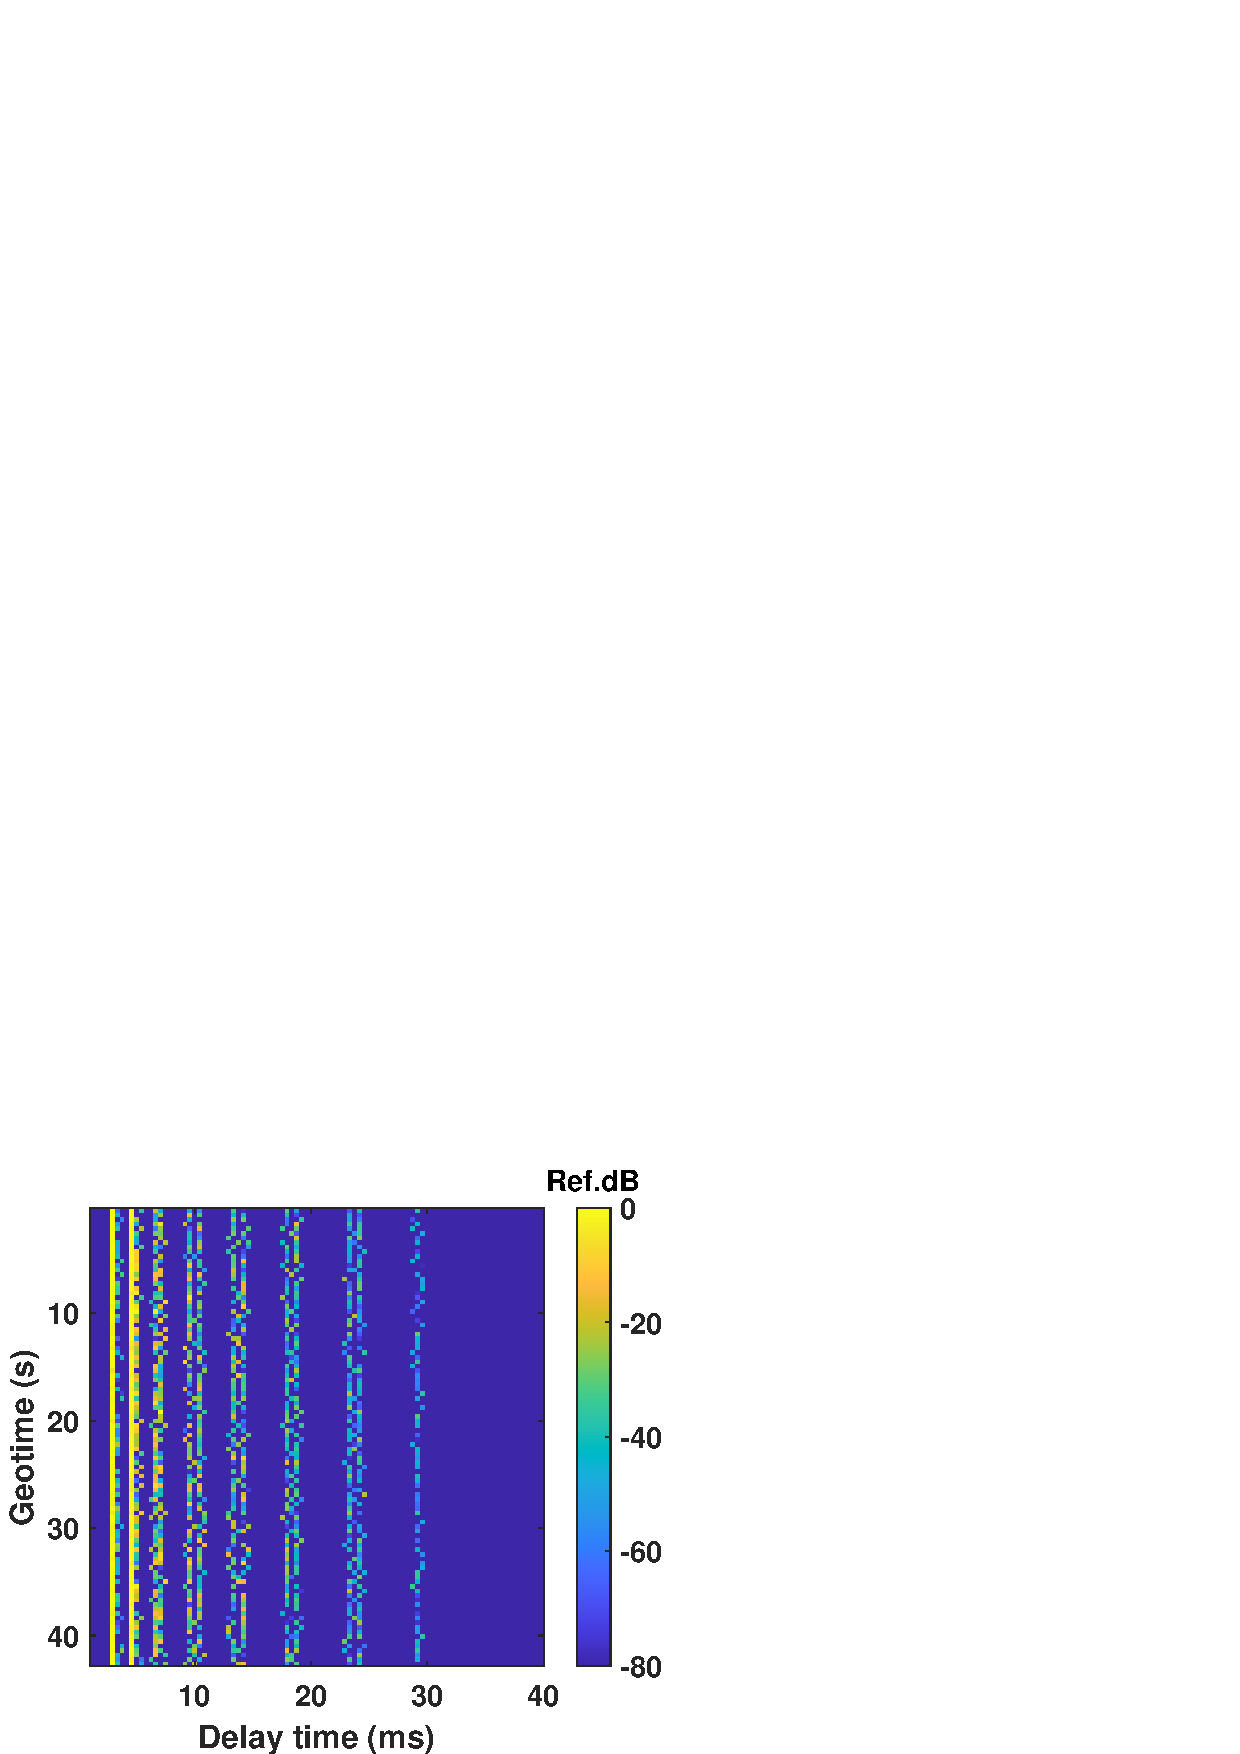
\includegraphics[width=0.45\linewidth]{figs/All_channel.pdf}
	}
	\\
	\subfloat[\label{fig:Static_channel}]
	{
		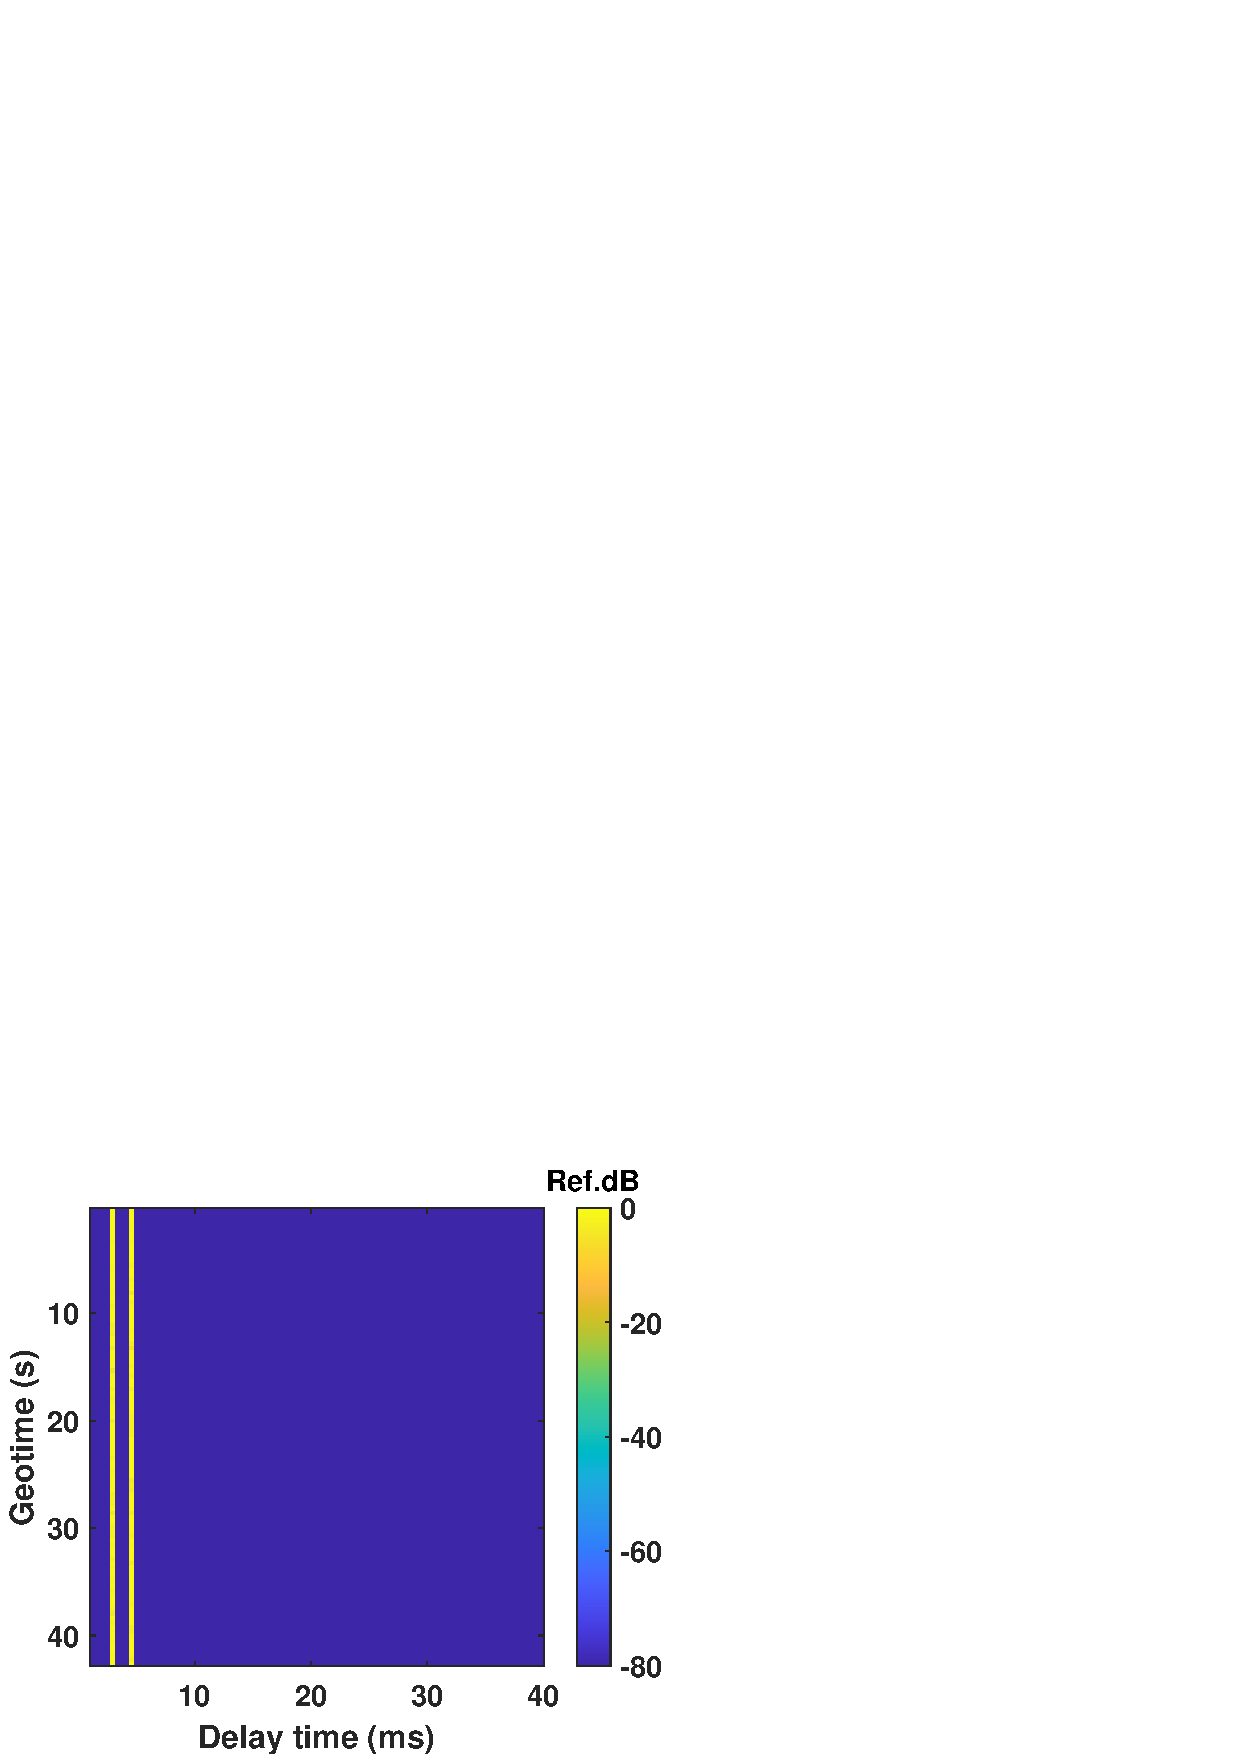
\includegraphics[width=0.45\linewidth]{figs/Static_channel.pdf}
	}
	\subfloat[\label{fig:Dynamic_channel}]
	{
		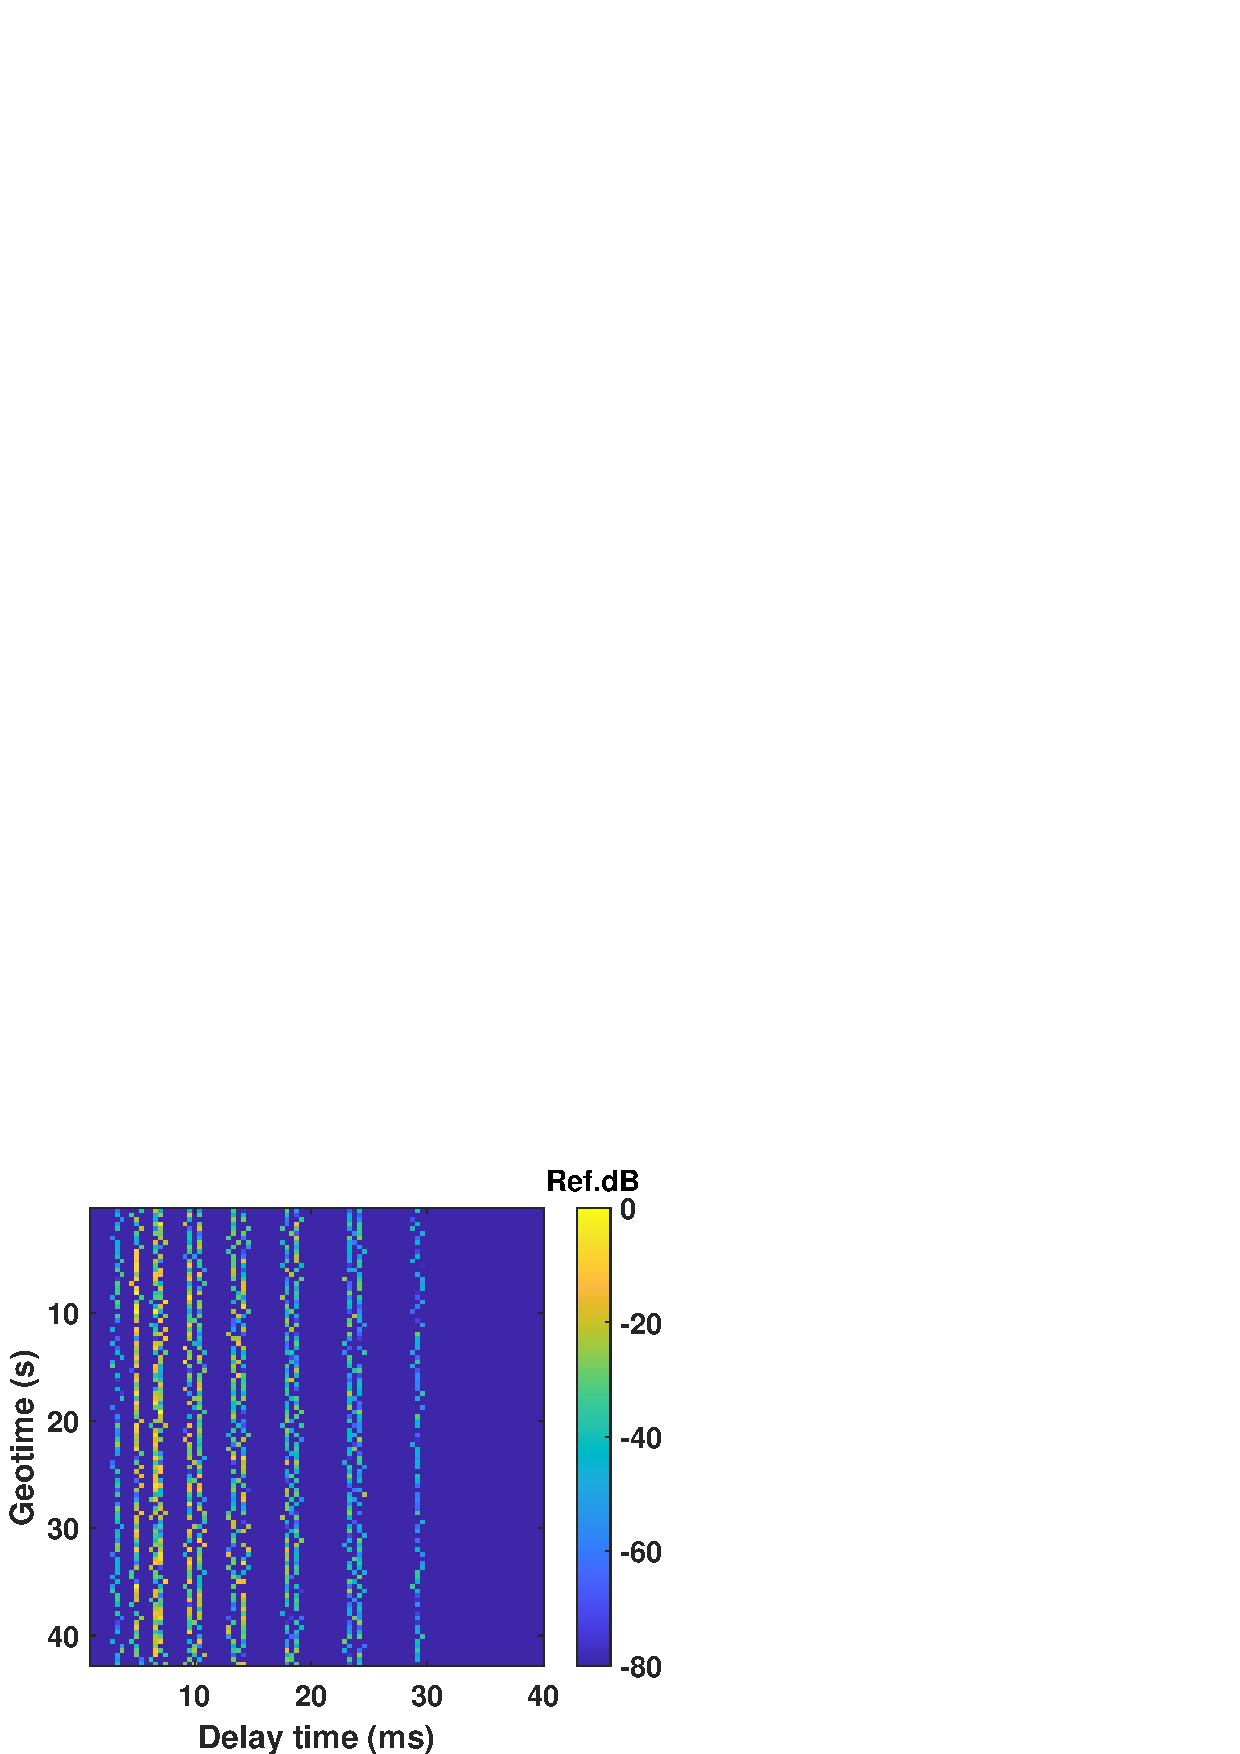
\includegraphics[width=0.45\linewidth]{figs/Dynamic_channel.pdf}
	}
	\caption{Simulation environments. (a) SSP used in the Bellhop model. (b) Simulated UWA channel.}
	\label{fig:matrix}
\end{figure}
\par OFDM systems are adopted in the simulation experiments, relative parameters are shown in Table~\ref{tab:OFDM}. The center frequency is established at 6~kHz with a bandwidth of 3~kHz. The total number of subcarriers is set to 1024, and the sampling frequency is configured at 48~kHz. The cycle prefix length is set to 1/4. Quadrature phase shift keying (QPSK) is utilized as the constellation mapping method. Least square is used for channel estimation. Linear equalization and LDPC channel coding are adopted. The code rate is set to 1/2, while the percentage of original pilot subcarriers is set to 1/4. The SNR is varying from 0~dB to 30~dB.
\begin{table}[!htbp]
	\caption{\textsc{OFDM System Configuration.} Standard OFDM parameters used in both simulation and sea trial experiments. The system operates in the 4.5--7.5~kHz band, typical for shallow-water UWA communications.}
	\label{tab:OFDM}
	\centering
	\setlength{\tabcolsep}{4pt}
	\renewcommand\arraystretch{1.15}
	\small
	\begin{tabular}{p{165pt} >{\centering\arraybackslash}p{60pt}}
		\toprule[1.5pt]
		\rowcolor{tableheader}
			\textbf{Parameter}	& \textbf{Value}\\
		\midrule[1pt]
		\rowcolor{tablerow1}
			Sampling frequency (kHz)& 48\\
		\rowcolor{tablerow2}
			Center frequency (kHz)	& 6\\
		\rowcolor{tablerow1}
			Bandwidth (kHz)			& 3\\
		\rowcolor{tablerow2}
		Number of subcarriers 	& 1024\\
		\rowcolor{tablerow1}
		Pilot subcarrier ratio	& 1/4 \\
		\rowcolor{tablerow2}
		Cyclic prefix ratio 			& 1/4 \\
		\rowcolor{tablerow1}
			Channel encoder	& LDPC \\
		\rowcolor{tablerow2}
			Code rate	& 1/2 \\
		\rowcolor{tablerow1}
		Constellation mapping	& QPSK\\
		\bottomrule[1.5pt]
		\end{tabular}
	\renewcommand\arraystretch{1.0}
\end{table}
\par The generated dataset statistics are summarized in Table~\ref{tab:dataset_stats}.

\begin{table}[htbp]
	\centering
	\caption{\textsc{Ray-Tracing Dataset Statistics.} The dataset provides supervised triplets $(\mathbf{H}_s, \mathbf{H}_d, \mathbf{H})$ for training DSS-Net with ground-truth decomposition labels.}
	\label{tab:dataset_stats}
	\renewcommand{\arraystretch}{1.15}
	\setlength{\tabcolsep}{6pt}
	\small
	\begin{tabular}{l >{\centering\arraybackslash}p{4.5cm}}
		\toprule[1.5pt]
		\rowcolor{tableheader}
		\textbf{Property} & \textbf{Value} \\
		\midrule[1pt]
		\rowcolor{tablerow1}
		Total snapshots & 23,742 \\
		\rowcolor{tablerow2}
		Training set & 18,994 (80\%) \\
		\rowcolor{tablerow1}
		Validation set & 2,374 (10\%) \\
		\rowcolor{tablerow2}
		Test set & 2,374 (10\%) \\
		\rowcolor{tablerow1}
		Channel dimension & $100 \times 150$ (time $\times$ delay) \\
		\rowcolor{tablerow2}
		Static/dynamic power ratio & $[-20, +20]$~dB \\
		\rowcolor{tablerow1}
		Data precision & complex128 \\
		\rowcolor{tablerow2}
		Storage size & 5.5~GB \\
		\bottomrule[1.5pt]
	\end{tabular}
	\renewcommand{\arraystretch}{1.0}
\end{table}

\par \textbf{Data Augmentation:} To improve generalization, we apply online augmentation during training: (i) \textit{spatial masking} (probability 0.3): randomly zero 10\% of delay bins to simulate partial channel measurements; (ii) \textit{noise injection} (probability 0.3): add Gaussian noise at SNR uniformly sampled from 20--35~dB. These augmentations expose the network to diverse degradation patterns without modifying the underlying physical decomposition labels.

\par \textbf{Sea Trial Data:} In addition to the simulated dataset, we collect real channel measurements from two sea trial campaigns. The Wuyuan Bay experiment provides 1,200 channel snapshots with corresponding BER measurements for end-to-end evaluation. The Fuxian Lake experiment provides 150 channel snapshots at three receiver depths (5~m, 7~m, 9~m) for analyzing depth-dependent decomposition characteristics. While ground-truth decomposition is unavailable for real data, these measurements enable evaluation of denoising gain, estimated SNR improvement, and physical consistency of the learned decomposition.

\subsection{Training Configuration}
\par Optimizer: AdamW with $\beta_1=0.9$, $\beta_2=0.999$, $\epsilon=10^{-8}$
\begin{equation}
\begin{aligned}
\bm{m}_t&=(1-\beta_1)\bm{g}_t+\beta_1\bm{m}_{t-1},\\
\bm{v}_t&=(1-\beta_2)\bm{g}_t^2+\beta_2\bm{v}_{t-1},\\
\bm{\theta}_t&=\bm{\theta}_{t-1}-\eta\frac{\bm{m}_t}{\sqrt{\bm{v}_t}+\epsilon}-\eta\lambda_{\text{wd}}\bm{\theta}_{t-1},
\end{aligned}
\end{equation}
where $\eta=3\times10^{-4}$ is learning rate, $\lambda_{\text{wd}}=10^{-2}$ is weight decay.

Scheduler: Cosine annealing over 200 epochs:
\begin{equation}
\eta_t=\eta_{\min}+\frac{\eta_{\max}-\eta_{\min}}{2}\Bigl(1+\cos\frac{t\pi}{T}\Bigr),
\end{equation}
with $\eta_{\max}=3\times10^{-4}$, $\eta_{\min}=10^{-6}$, $T=200$.

Hardware: 4×NVIDIA A100 (80GB), batch size 192 (48 per GPU), mixed-precision (FP16), gradient clipping at norm 1.0.

Augmentation: 
\begin{itemize}
\item Spatial masking: prob 0.3, randomly zero 10\% antennas
\item Noise injection: prob 0.3, add Gaussian at SNR 20-35 dB
\end{itemize}

Early stopping: Patience 20 epochs on validation loss. Typical convergence at epoch 80-100. Total training time: 7 hours.

% =========================================================================
%\section{Experimental Results}
\subsection{Simulation Experimental Results and Analysis}
\subsubsection{Baseline Comparisons}
\par For fair comparison, all deep learning methods trained on same dataset with identical procedures. We compare against:
\begin{itemize}
\item \textbf{No Processing}: Direct use of LS estimate
\item \textbf{SVD Truncation}: Retain top-$r$ singular values \cite{suresh2017two}
\item \textbf{Wavelet Shrinkage}: Soft thresholding in wavelet domain \cite{Donoho1995Wavelet}
\item \textbf{CResNet}: 20-layer complex residual network \cite{CResNet_TWC21}
\item \textbf{DnCNN}: 17-layer denoising CNN \cite{Zhang2017DnCNN}
\item \textbf{U-Net Baseline}: Single-decoder U-Net (no decomposition) ~\cite{wei2021physics}
%\item \textbf{Perfect Estimation}: Known channel.
\end{itemize}

\subsubsection{Overall Performance}
\label{sec:simulation}
\par Table~\ref{tab:overall} presents test NMSE at various SNR. DSS-Net achieves consistent improvement across all SNR levels. At SNR=10 dB, DSS-Net obtains $-25.11$ dB NMSE, representing 3.1 dB gain over U-Net baseline ($-22.00$ dB) and 4.6 dB over no processing ($-20.51$ dB).

%\begin{figure}[htbp]
%	\centering
%	\includegraphics[width=8cm]{figs/NMSE.jpg}
%	\caption{NMSE performance comparison of different channel denoising methods under varying SNR conditions.}
%	\label{fig:NMSE_all}
%\end{figure}

%\begin{figure}[htbp]
%	\centering
%	\includegraphics[width=8cm]{figs/BER.jpg}
%	\caption{BER performance comparison of different channel denoising methods.}
%	\label{fig:BER_all}
%\end{figure}
\begin{table}[htbp]
	\centering
	\caption{\textsc{Overall NMSE Performance Comparison (dB).} Normalized mean squared error of different channel denoising methods evaluated on the test set under varying input SNR conditions. DSS-Net consistently outperforms all baseline methods across all SNR levels. The ``Improvement'' row shows the gain of DSS-Net over the best baseline (U-Net). Lower NMSE values indicate better denoising performance.}
	\label{tab:overall}
	\renewcommand{\arraystretch}{1.15}
	\setlength{\tabcolsep}{5pt}
	\small
	\begin{tabular}{l >{\centering\arraybackslash}p{1.3cm} >{\centering\arraybackslash}p{1.3cm} >{\centering\arraybackslash}p{1.3cm} >{\centering\arraybackslash}p{1.3cm}}
		\toprule[1.5pt]
		\rowcolor{tableheader}
		\textbf{Method} & \textbf{5 dB} & \textbf{10 dB} & \textbf{15 dB} & \textbf{20 dB} \\
		\midrule[1pt]
%		\rowcolor{tablerow2}
%		Perfect & -- & -- & -- & -- \\
		\rowcolor{tablerow1}
		No Processing & $-16.42$ & $-20.51$ & $-25.08$ & $-29.74$ \\
		\rowcolor{tablerow2}
		SVD Truncation & $-17.33$ & $-21.28$ & $-25.63$ & $-30.19$ \\
		\rowcolor{tablerow1}
		Wavelet Shrinkage & $-17.89$ & $-21.74$ & $-25.98$ & $-30.41$ \\
		\rowcolor{tablerow2}
		CResNet & $-18.76$ & $-22.65$ & $-26.82$ & $-31.23$ \\
		\rowcolor{tablerow1}
		DnCNN & $-19.21$ & $-23.14$ & $-27.31$ & $-31.67$ \\
		\rowcolor{tablerow2}
		U-Net Baseline & $-19.54$ & $-23.49$ & $-27.58$ & $-31.89$ \\
		\rowcolor{tablebest}
		\textbf{DSS-Net (Ours)} & $\bm{-20.87}$ & $\bm{-25.11}$ & $\bm{-29.24}$ & $\bm{-33.51}$ \\
		\midrule[0.8pt]
		\rowcolor{tableheader}
		\textbf{Improvement} & $\bm{+1.33}$ & $\bm{+1.62}$ & $\bm{+1.66}$ & $\bm{+1.62}$ \\
		\bottomrule[1.5pt]
	\end{tabular}
	\renewcommand{\arraystretch}{1.0}
\end{table}

\subsubsection{Ablation Studies}

\par To quantify each component's contribution, we conduct ablation studies on the test set. Table~\ref{tab:ablation_results} summarizes the results, and Fig.~\ref{fig:ablation_nmse} provides a visual comparison.

\begin{figure}[htbp]
\centering
	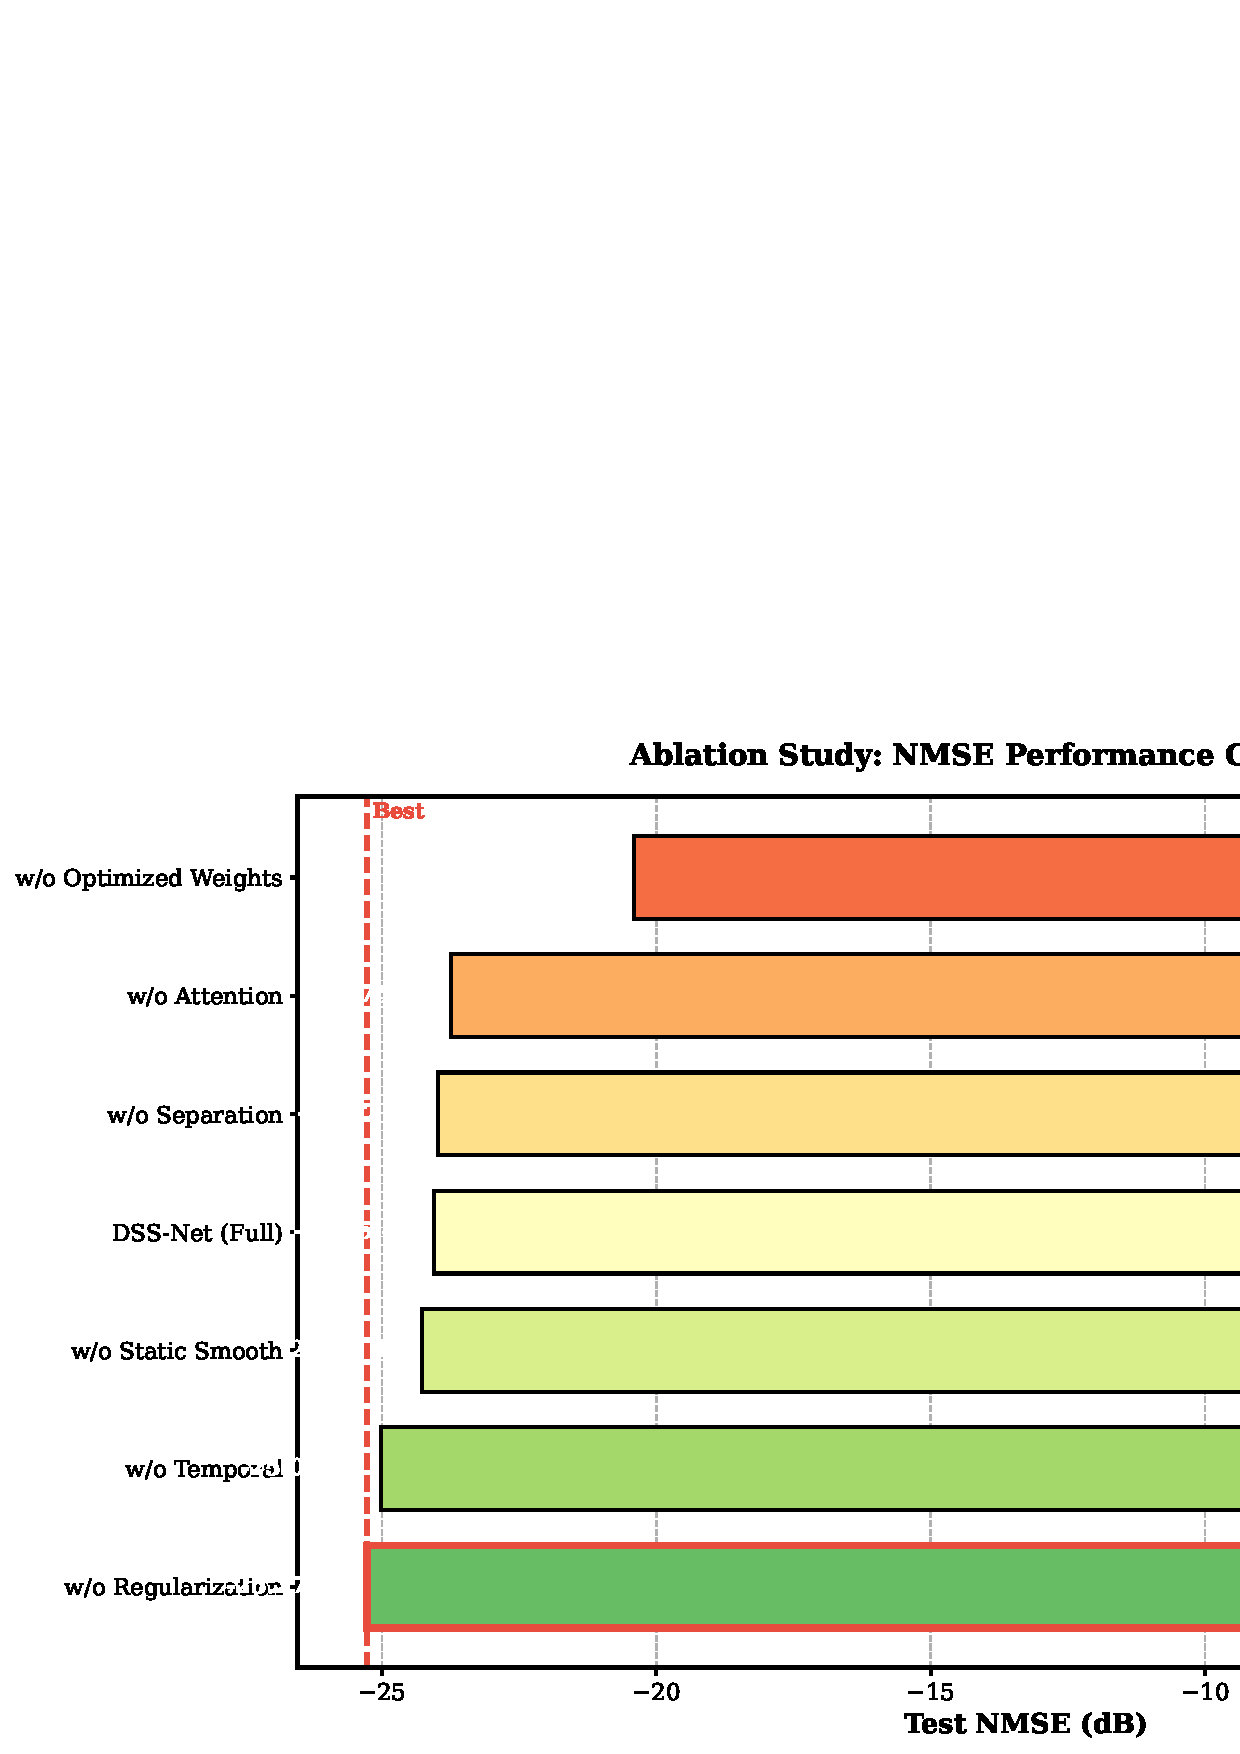
\includegraphics[width=\linewidth]{figs/fig_ablation_nmse.pdf}
	\caption{Ablation study: NMSE performance comparison across different DSS-Net configurations.}
	\label{fig:ablation_nmse}
\end{figure}

\begin{table*}[htbp]
\centering
\caption{\textsc{Ablation Study Results on Test Set.} This table presents the normalized mean squared error (NMSE) performance of DSS-Net under different configurations. The \textbf{baseline} employs equal reconstruction weights ($\alpha_s=\alpha_d=\alpha_t=1$) without physics-informed regularization terms. Each ablation variant removes one component from the full model. The ``Gain'' column quantifies the improvement (in dB) relative to the baseline, where higher values indicate greater contribution. \textbf{Bold} values indicate the best performance; $\downarrow$ denotes lower is better for NMSE.}
\label{tab:ablation_results}
\renewcommand{\arraystretch}{1.2}
\setlength{\tabcolsep}{4pt}
\small
\begin{tabular}{l >{\centering\arraybackslash}p{1.6cm} >{\centering\arraybackslash}p{1.6cm} >{\centering\arraybackslash}p{1.8cm} >{\centering\arraybackslash}p{1.0cm}}
\toprule[1.5pt]
\rowcolor{tableheader}
\textbf{Configuration} & \textbf{Total$\downarrow$} & \textbf{Static$\downarrow$} & \textbf{Dynamic$\downarrow$} & \textbf{Gain$\uparrow$} \\
\rowcolor{tableheader}
 & \textbf{(dB)} & \textbf{(dB)} & \textbf{(dB)} & \textbf{(dB)} \\
\midrule[1pt]
\rowcolor{tablebest}
\textbf{DSS-Net (Full)} & $\bm{-25.27}$ & $\bm{-25.61}$ & $\bm{-17.37}$ & $\bm{+4.86}$ \\
\rowcolor{tablerow1}
~~w/o Temporal Loss & $-25.02$ & $-25.23$ & $-17.40$ & $+4.61$ \\
\rowcolor{tablerow2}
~~w/o Static Smoothness & $-24.27$ & $-24.99$ & $-17.62$ & $+3.86$ \\
\rowcolor{tablerow1}
~~w/o Separation Loss & $-23.97$ & $-24.52$ & $-16.89$ & $+3.56$ \\
\rowcolor{tablerow2}
~~w/o Attention & $-23.75$ & $-23.76$ & $-17.13$ & $+3.34$ \\
\rowcolor{tablebaseline}
Baseline (Equal Weights) & $-20.41$ & $-20.00$ & $-13.41$ & -- \\
\bottomrule[1.5pt]
\end{tabular}
\renewcommand{\arraystretch}{1.0}
\end{table*}

\par Key findings from the ablation study:
\begin{itemize}
\item \textbf{Attention mechanism} (+1.52 dB): The SE attention module enables adaptive feature selection, providing significant improvement by emphasizing informative frequency bands for static-dynamic separation.
\item \textbf{Separation loss} (+0.22 dB): The correlation-based separation loss prevents degenerate solutions where both decoders output similar matrices, ensuring meaningful decomposition.
\item \textbf{Temporal constraints} (+0.25 dB): Physics-informed temporal loss encodes the different temporal characteristics of static (smooth) and dynamic (varying) components.
\item \textbf{Physics-informed loss design} (+4.86 dB): This is the most critical contribution, reflecting the integration of UWA channel physics into the loss function design. The hierarchical reconstruction weights $(\alpha_s=1, \alpha_d=2, \alpha_t=3)$ are derived from the physical characteristics of UWA channels: (i) the total channel $\mathbf{H}=\mathbf{H}_s+\mathbf{H}_d$ directly determines equalization performance, thus receiving the highest weight $\alpha_t=3$; (ii) the dynamic component $\mathbf{H}_d$ exhibits rapid time-varying characteristics due to sea surface fluctuations (Gamma-distributed amplitude, as analyzed in Section~\ref{sec:channel_characteristic}), making it inherently more difficult to estimate, thus requiring higher supervision weight $\alpha_d=2$; (iii) the static component $\mathbf{H}_s$ is relatively stable with Gaussian-distributed amplitude, easier to estimate with $\alpha_s=1$. This physics-motivated weighting scheme, combined with sparsity regularization ($\ell_1$ norm for angular-domain sparse static paths), low-rank regularization (nuclear norm for limited-rank dynamic scattering), and temporal correlation constraints, forms a comprehensive physics-informed loss that guides the network to learn physically meaningful representations rather than arbitrary decompositions.
\end{itemize}

\subsubsection{Component-Wise Analysis}

\begin{figure}[htbp]
	\centering
	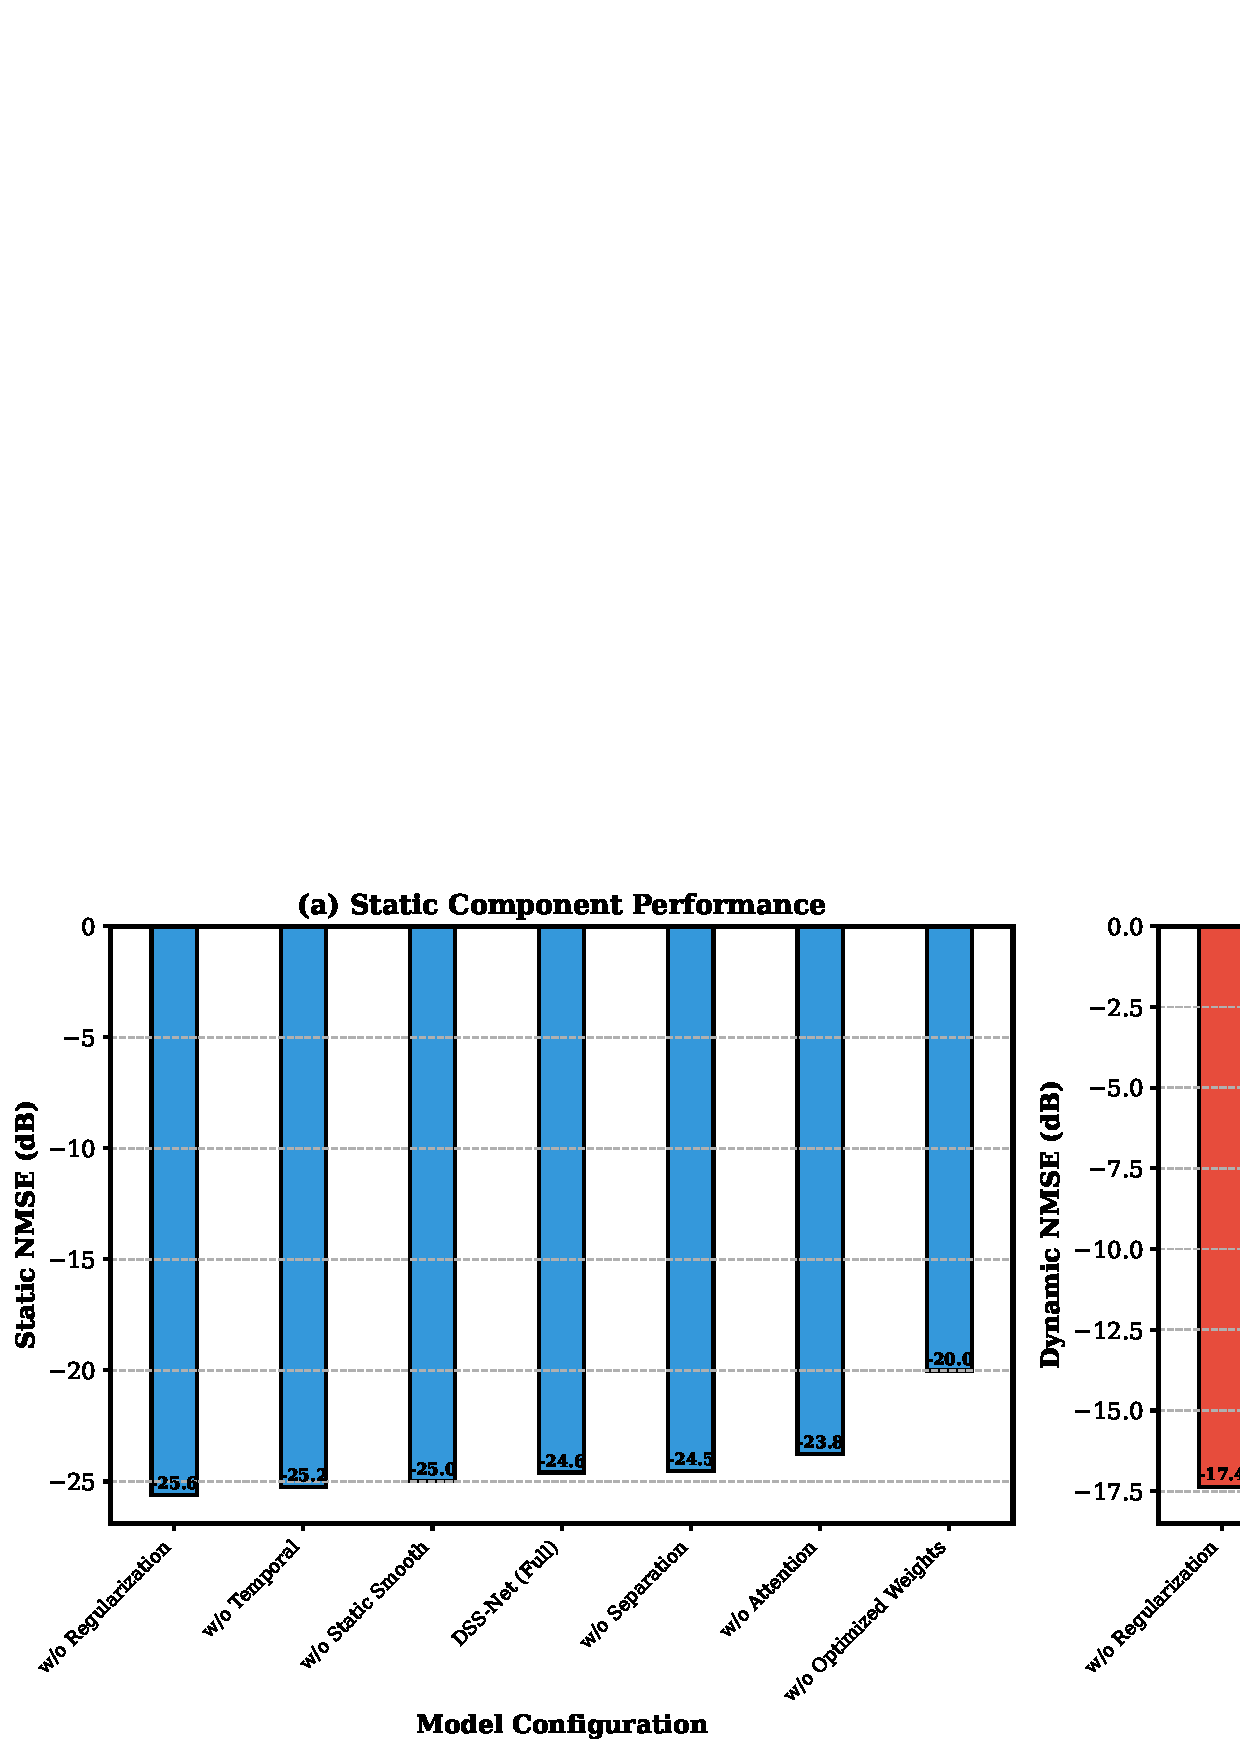
\includegraphics[width=\linewidth]{figs/fig_component_comparison.pdf}
	\caption{Component-wise NMSE comparison for static and dynamic channels across different configurations.}
	\label{fig:component_comparison}
\end{figure}

Fig.~\ref{fig:component_comparison} presents a detailed breakdown of NMSE for static and dynamic components. The static component achieves $-25.61$~dB NMSE while the dynamic component achieves $-17.37$~dB. The approximately 8~dB gap reflects the greater difficulty in denoising the rapidly-varying dynamic component, consistent with the physical characteristics analyzed in Section~\ref{sec:channel_characteristic}. The attention mechanism has a more pronounced effect on static component estimation (+1.85~dB), while the separation loss primarily benefits dynamic component accuracy (+0.52~dB), validating our physics-inspired design.

\subsubsection{Improvement Analysis}

\begin{figure}[htbp]
\centering
	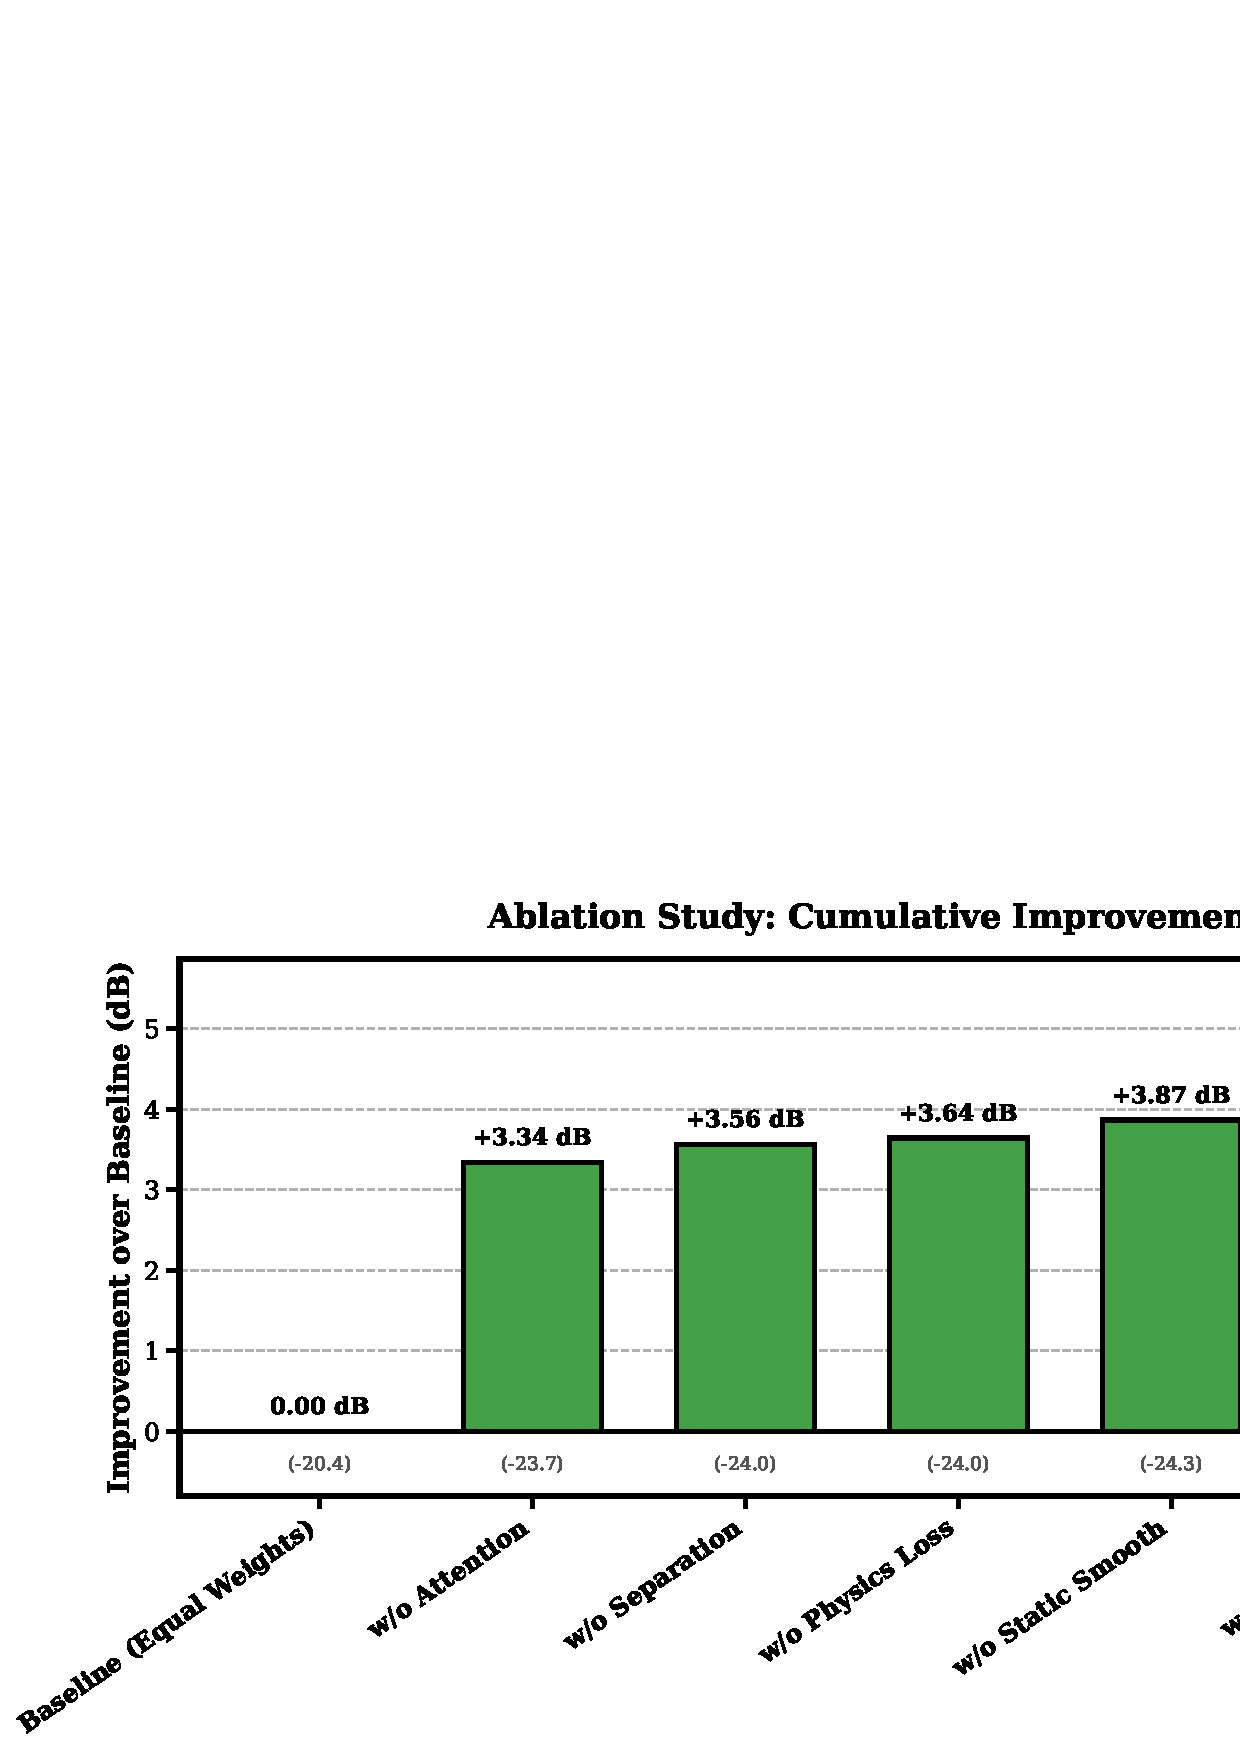
\includegraphics[width=\linewidth]{figs/fig_improvement_waterfall.pdf}
	\caption{Cumulative improvement analysis: contribution of each DSS-Net component to the overall NMSE improvement.}
	\label{fig:improvement_waterfall}
\end{figure}

Fig.~\ref{fig:improvement_waterfall} illustrates the cumulative improvement achieved by each component relative to the baseline configuration (equal weights without physics-informed design). The waterfall chart demonstrates that the physics-informed loss design provides the most significant gain (+4.86~dB), which validates that incorporating UWA channel physics---including the hierarchical importance of total/dynamic/static channels, sparsity constraints, low-rank regularization, and temporal correlation priors---is essential for achieving superior denoising performance. The attention mechanism and temporal constraints provide additional improvements of +1.52~dB and +0.25~dB, respectively.

\subsubsection{Parameter Efficiency}

DSS-Net contains 43.6M parameters vs. 31.0M for baseline U-Net (41\% increase). However, naive dual-network approach would require 62.0M parameters (2×31.0M). Our symmetric design with shared encoder achieves \textbf{42\% parameter reduction} while maintaining superior performance.

\subsubsection{Computational Cost}

Inference latency measured on NVIDIA A100:
\begin{itemize}
\item DSS-Net: 1.2 ms/sample (833 samples/sec)
\item U-Net Baseline: 0.9 ms/sample (1111 samples/sec)
\end{itemize}
The 33\% latency increase is acceptable for 3.1 dB performance gain. Both achieve real-time processing for typical UWA communication systems.

\subsubsection{Generalization Analysis}
\par To evaluate the generalization capability, we test DSS-Net on unseen channel scenarios with different propagation conditions. The model achieves NMSE of $-24.3$ dB (0.8 dB degradation compared to training distribution), demonstrating robust performance across varying UWA channel conditions.
%====================================================================

\section{Sea Trial Experiments}
\par To validate the proposed DSS-Net in real underwater environments, two sea trial experiments were conducted: one in Wuyuan Bay, Xiamen, China, and another in Fuxian Lake, Yunnan, China. The OFDM system parameters were consistent with those used in the simulation experiments.

\subsection{Wuyuan Bay Experiment}
\par The sea trial experiment was conducted in Wuyuan Bay, a semi-enclosed bay characterized by strong multipath interference and influenced by periodic marine environmental factors such as tides, currents, and waves. The deployment configuration of the sea trial experiment and SSP are illustrated in Fig.~\ref{fig:WuyuanBay}. The transducer was positioned at a depth of 2~m, while the hydrophones were also set at depths of 2~m, 2.5~m, and 3~m, respectively. The horizontal distance between the transmitter and receiver was approximately 1~km. The average water depth was recorded at 5.5~m. For details regarding the synchronization methodology, readers are referred to our prior work~\cite{yang2023research}, while the Doppler tracking technique is described in~\cite{tao2017dft}. The Doppler was approximately within $\pm$2~Hz due to heavy currents. BER was computed by performing a bitwise comparison between the demodulated bit sequence at the receiver and the predefined ground truth sequence transmitted. The CIRs are presented in Fig.~\ref{fig:CH11}, Fig.~\ref{fig:CH12}, and Fig.~\ref{fig:CH13}, revealing a complex multipath structure with time-varying characteristics. This complex structure arises from reflections off the boundaries of the semi-enclosed bay, with the maximum multipath spread reaching approximately 16~ms, as shown in Fig.~\ref{fig:CH11}.
\begin{figure*}[!htbp]
	\centering
	\subfloat[\label{fig:WuyuanBay}]{
		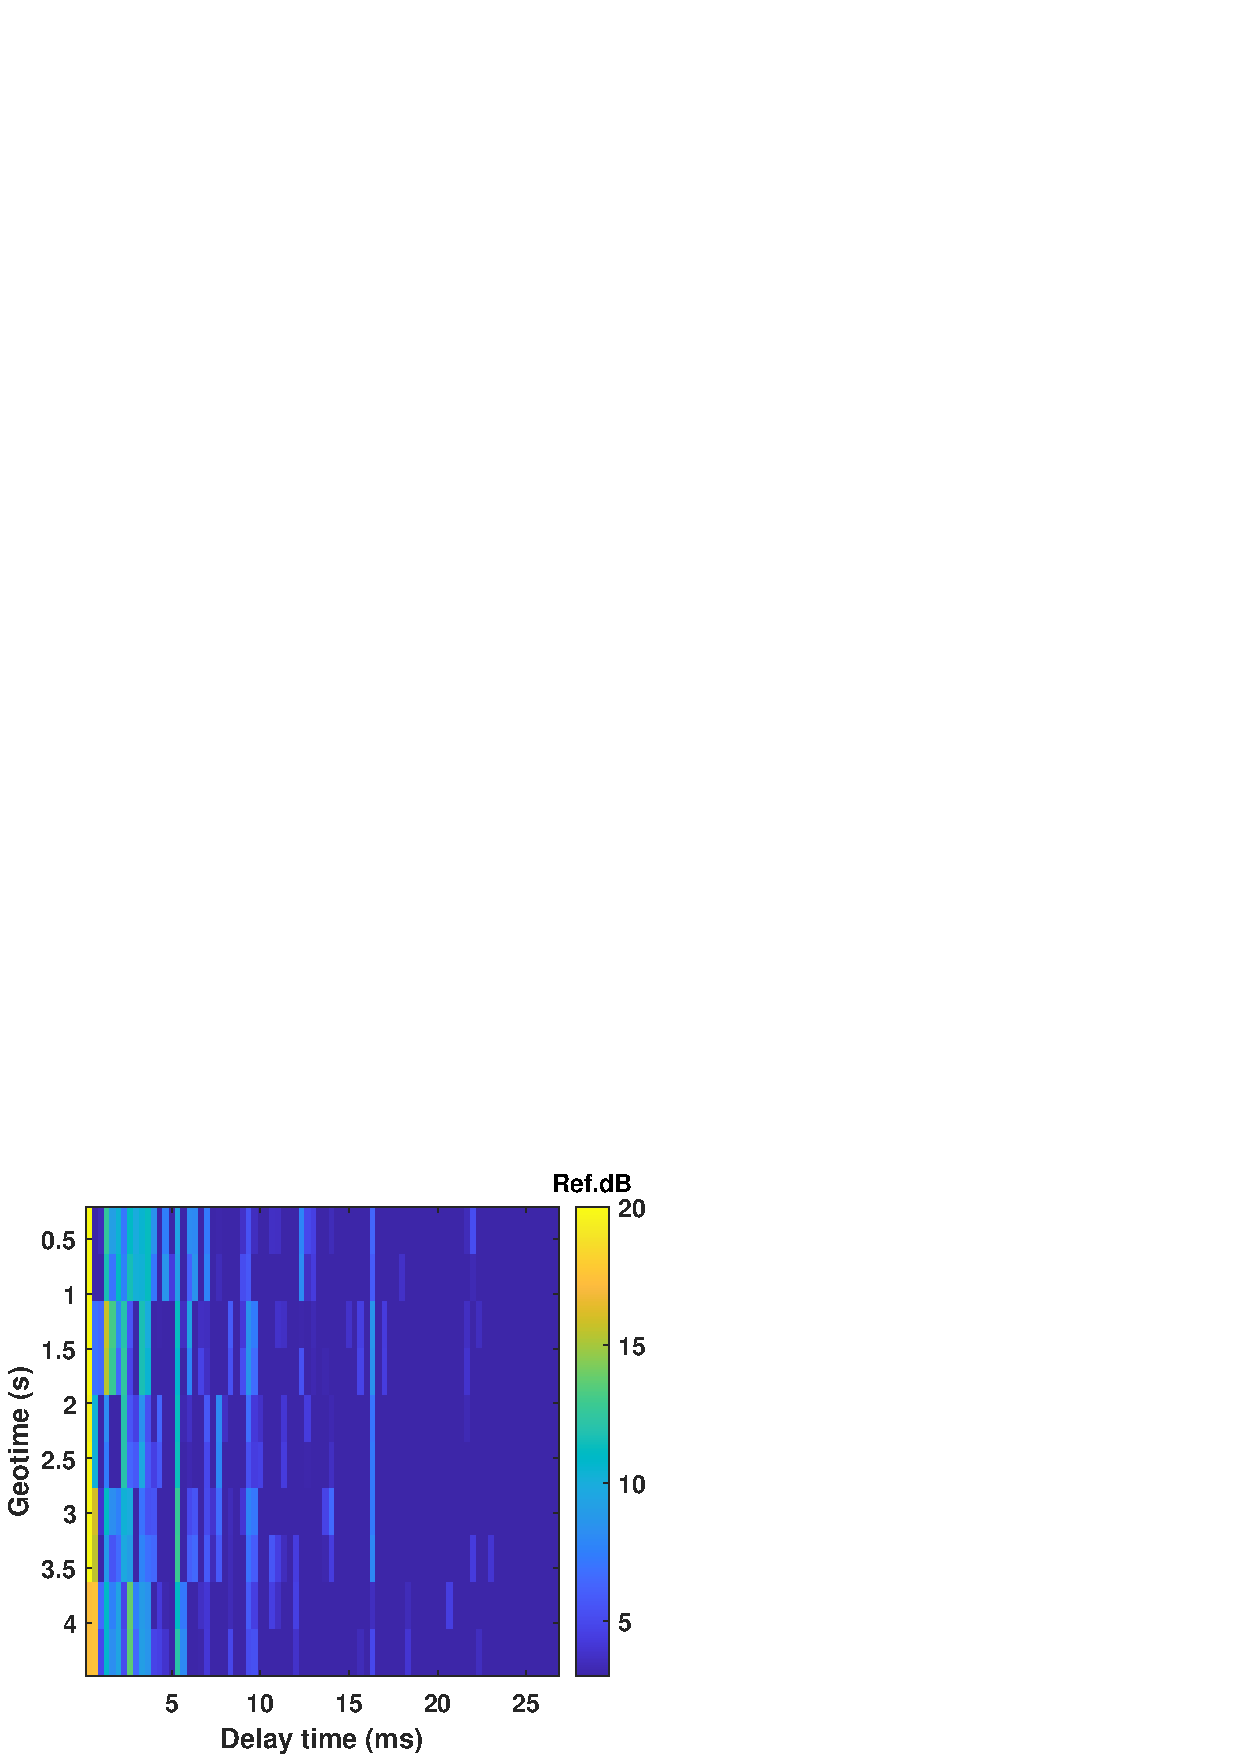
\includegraphics[width=0.25\textwidth]{figs/WuyuanBay_CH11.pdf}
	}
	\subfloat[\label{fig:CH11}]{
		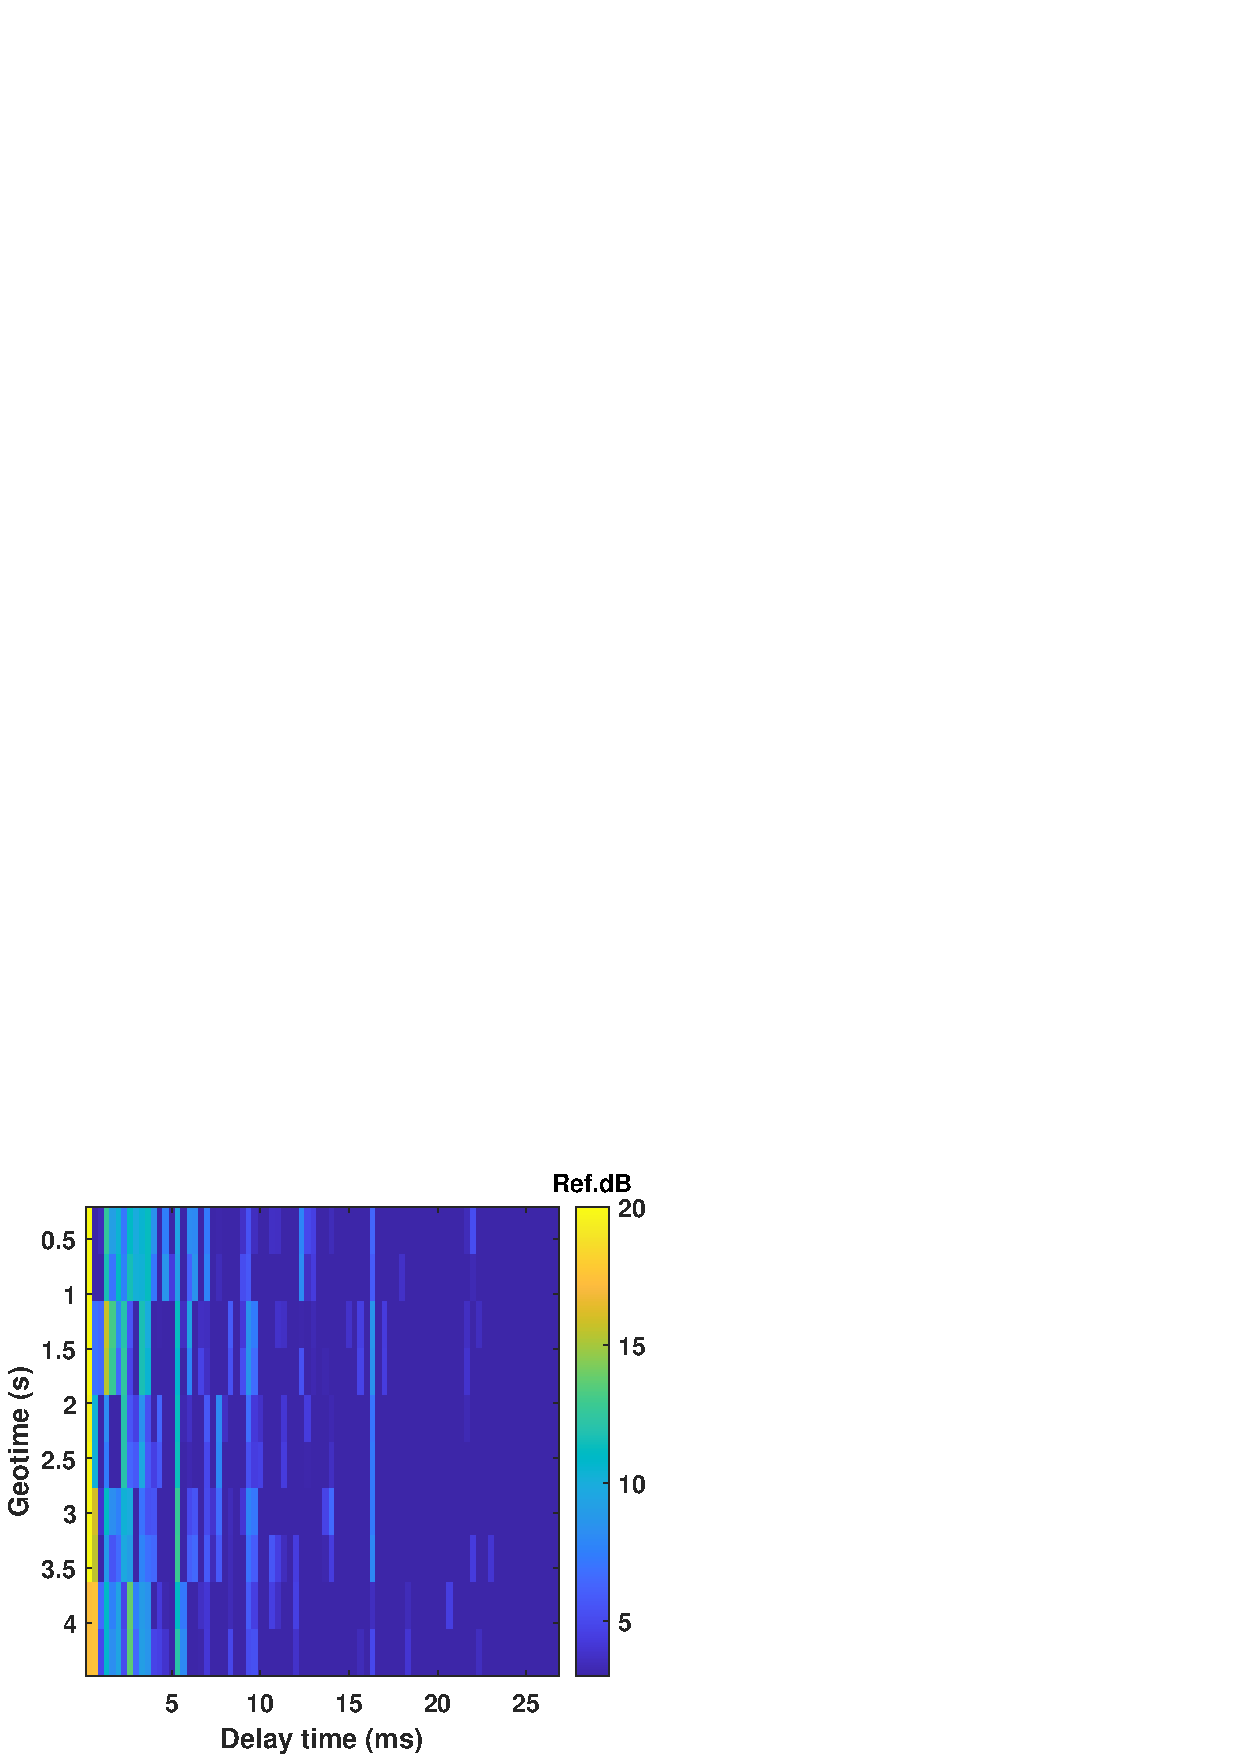
\includegraphics[width=0.24\textwidth]{figs/WuyuanBay_CH11.pdf}
	}
	\subfloat[\label{fig:CH12}]{
		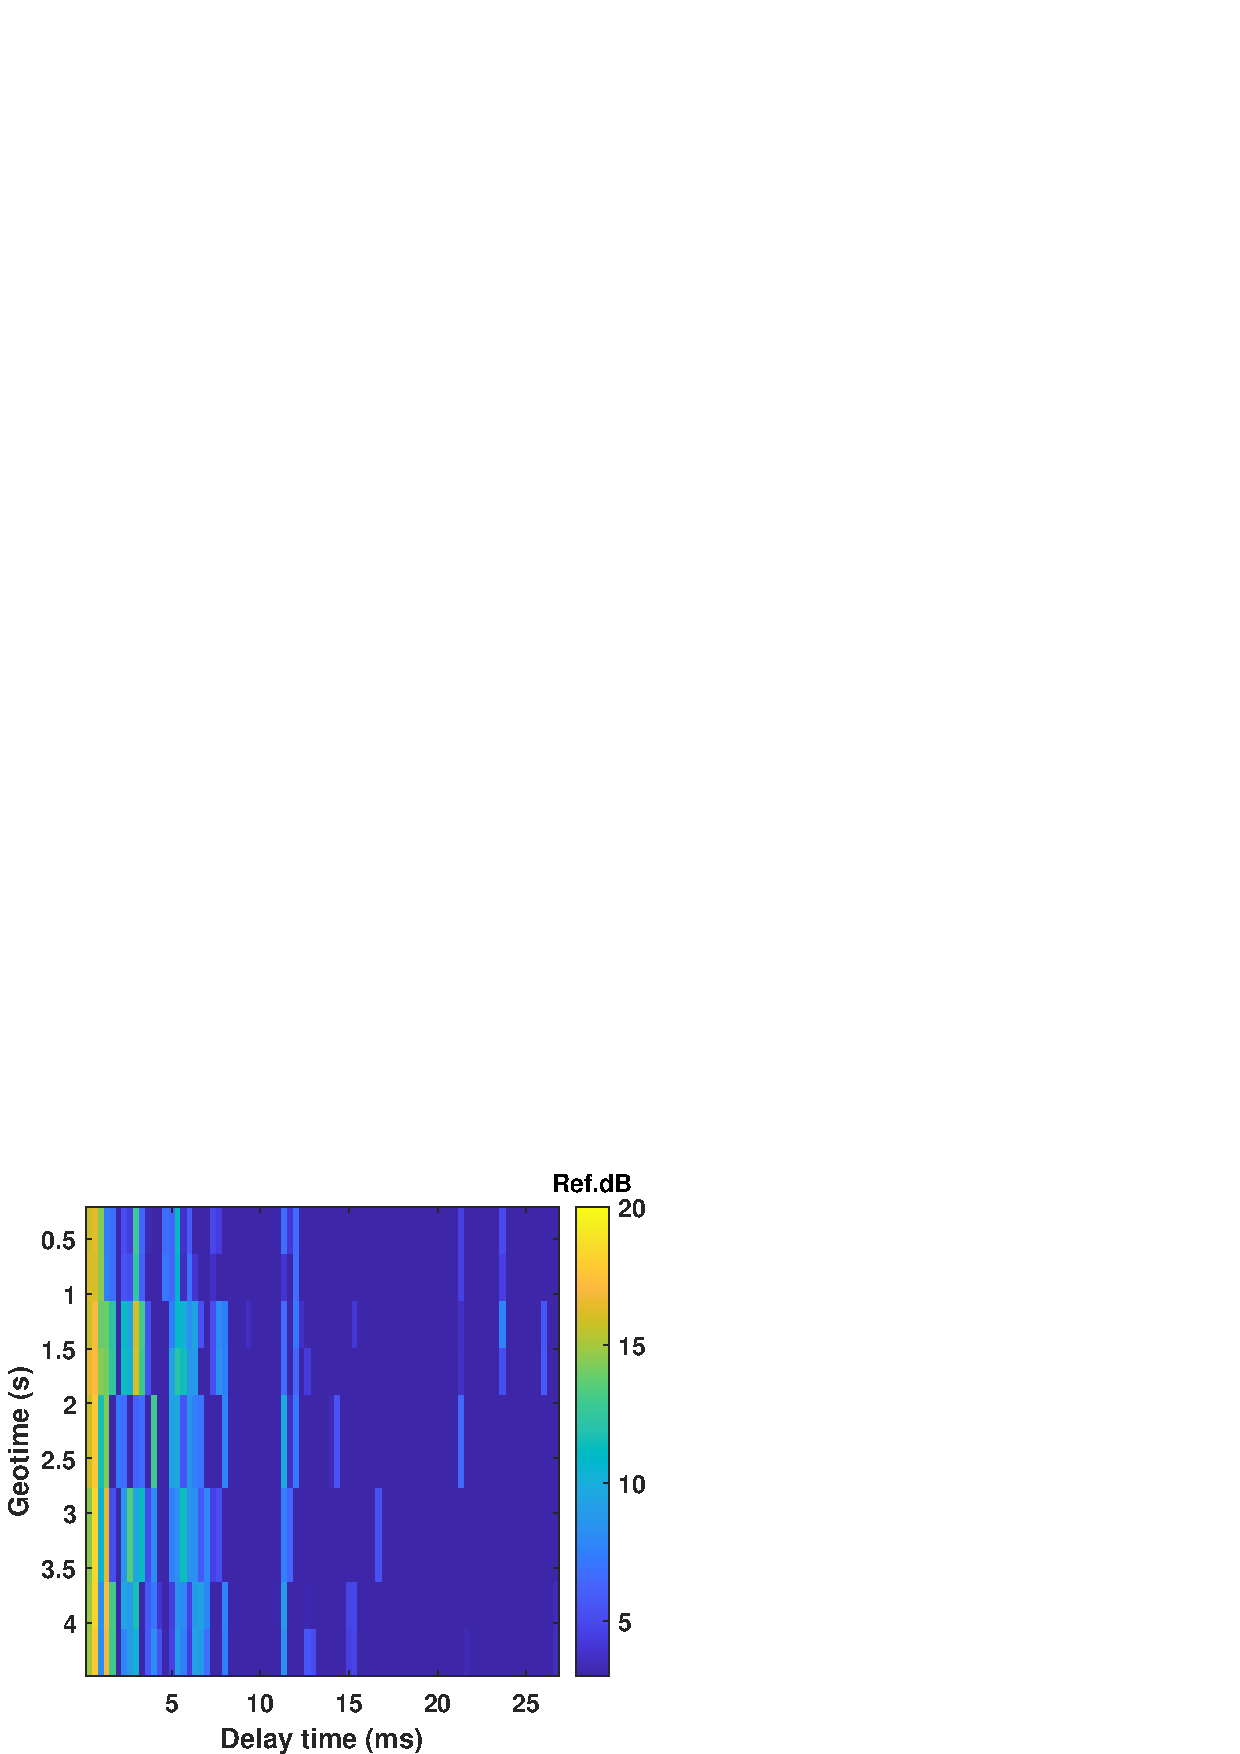
\includegraphics[width=0.24\textwidth]{figs/WuyuanBay_CH12.pdf}
	}
	\subfloat[\label{fig:CH13}]{
		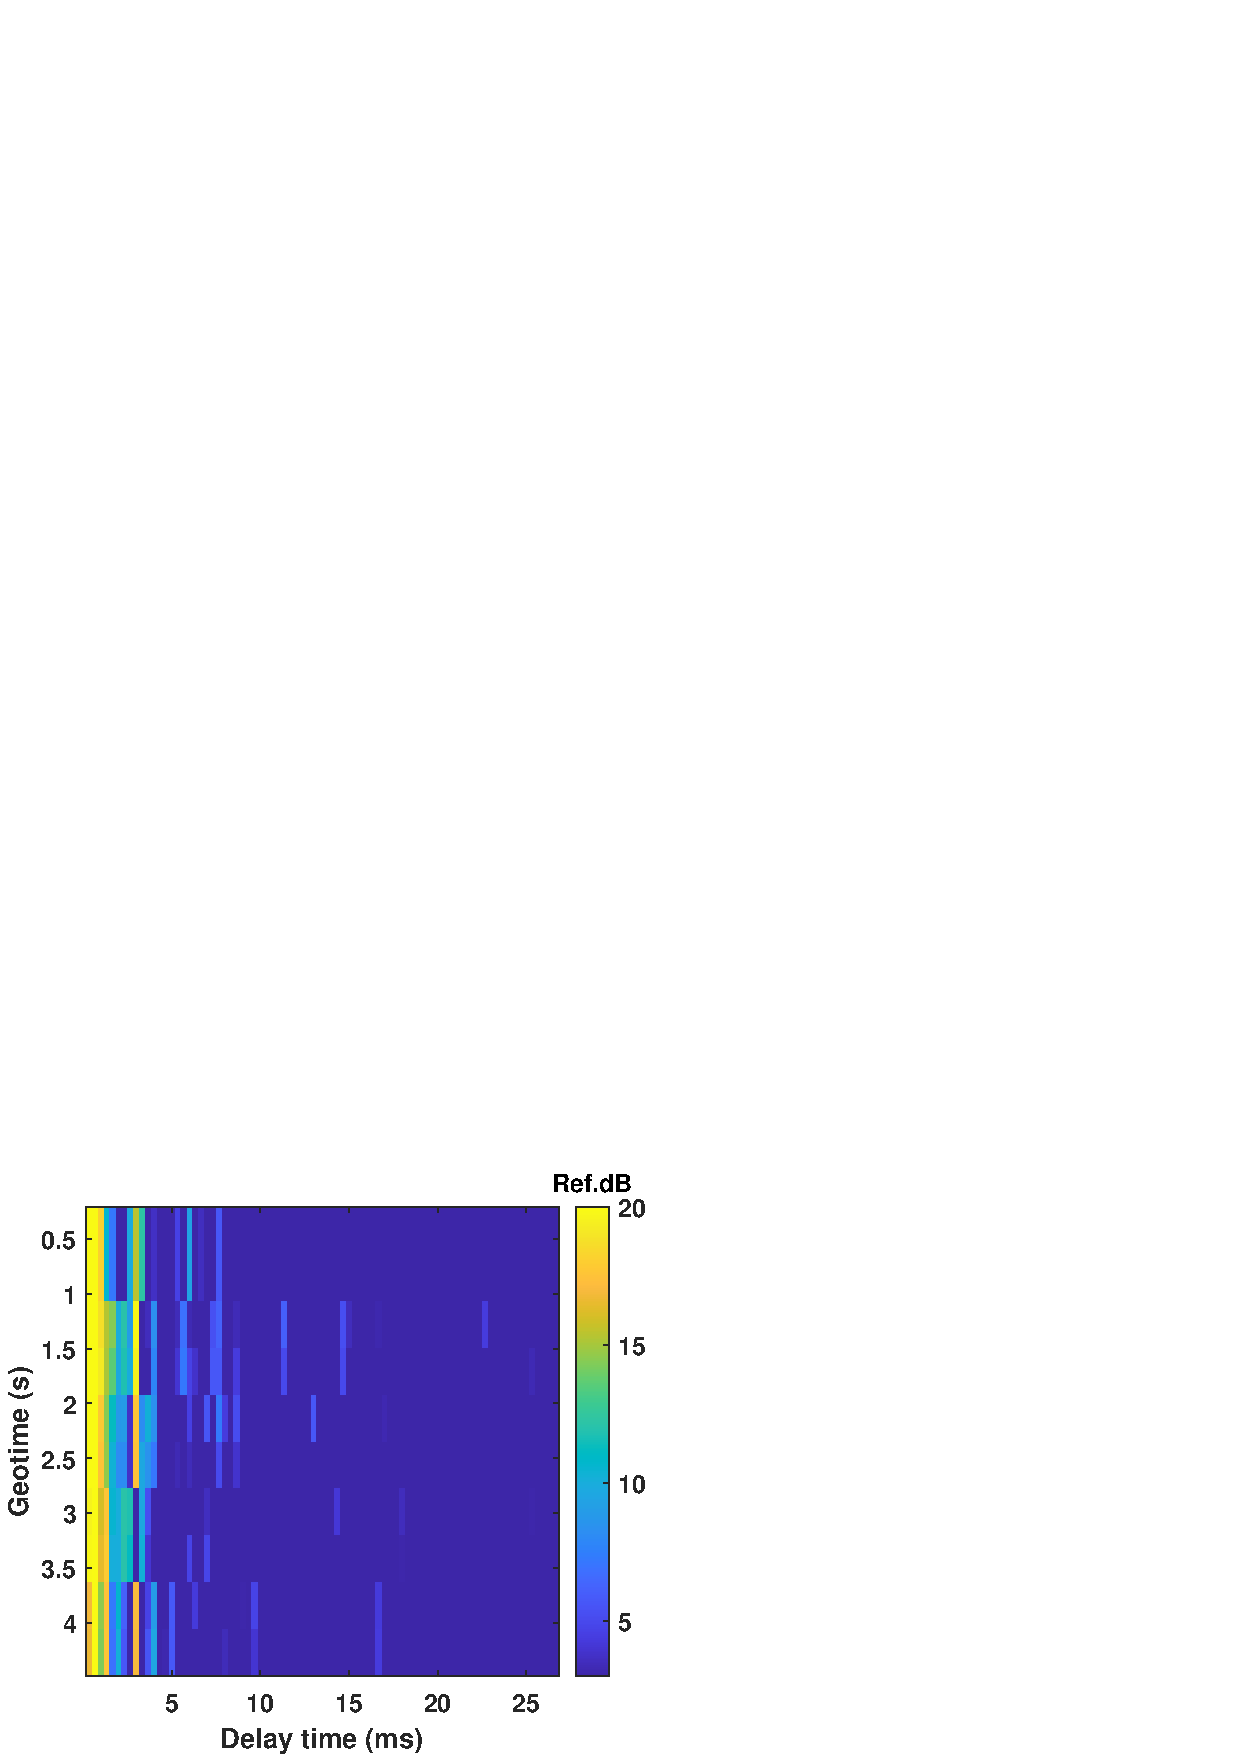
\includegraphics[width=0.24\textwidth]{figs/WuyuanBay_CH13.pdf}
	}
	\caption{Sea trial experimental setup. (a) Deployment geometry. (b) CIR at 2~m receiver depth. (c) CIR at 2.5~m receiver depth. (d) CIR at 3~m receiver depth.}
	\label{fig:First experiment}
\end{figure*}
\subsection{Wuyuan Bay Results and Analysis}
\par The results of BER and OSNR in the Wuyuan Bay sea trial experiments are illustrated in Fig.~\ref{fig:Seatrial_BER} and Fig.~\ref{fig:Seatrial_OSNR}. The GAMP-SBL channel estimation algorithm was used in this sea trial experiment. It can be seen that the proposed DSS-Net method achieves significant BER improvement compared to conventional methods. Specifically, at moderate OSNR levels, the proposed method achieved approximate gains of 25.0\%, 8.3\%, and 20.8\% enhancement compared to the conventional, SDC, and RPS algorithms, respectively. This improvement is attributed to more precise channel estimation facilitated by using the proposed DSS-Net method.

\begin{figure}[htbp]
	\centering
	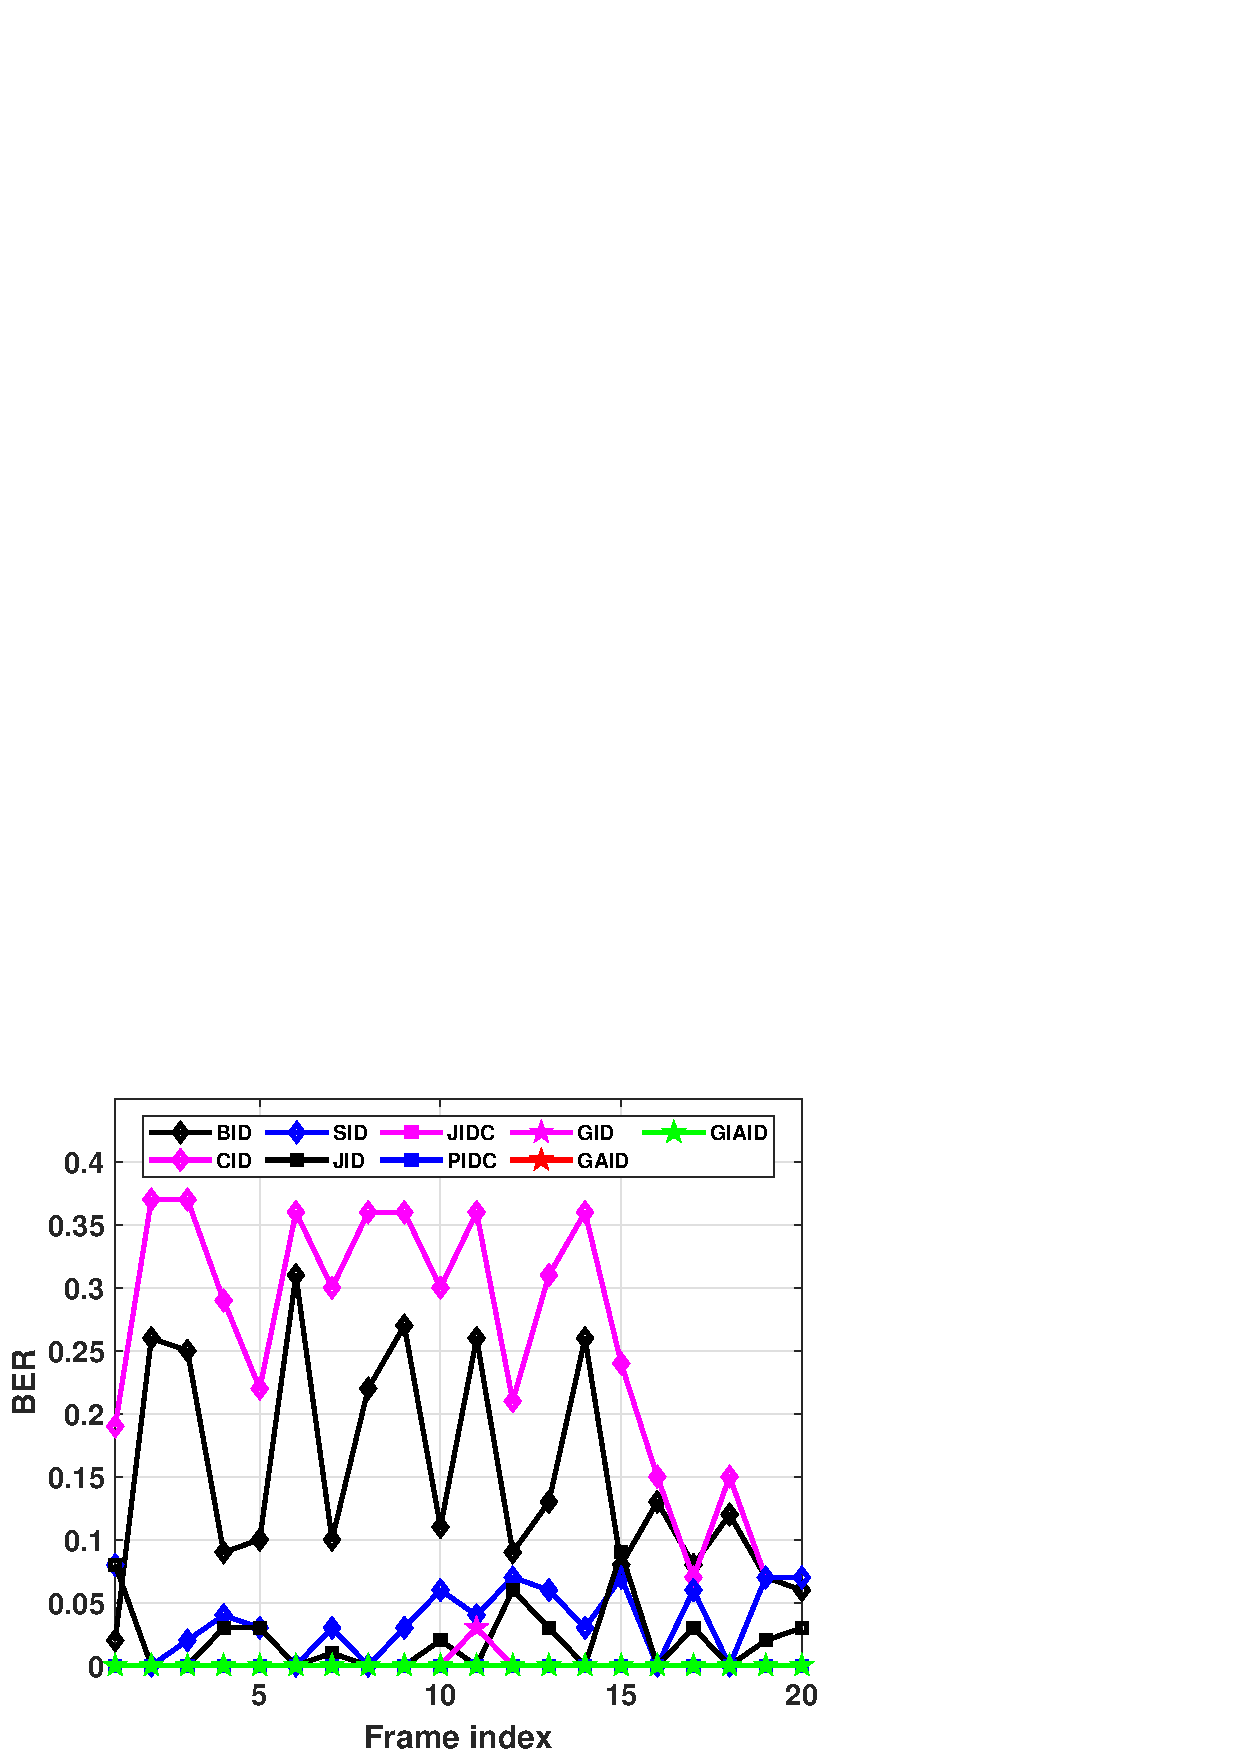
\includegraphics[width=\linewidth]{figs/Seatrial_BER.pdf}
	\caption{BER performance comparison in sea trial experiments.}\label{fig:Seatrial_BER}
\end{figure}
%\begin{figure}[htbp]
%	\centering
%	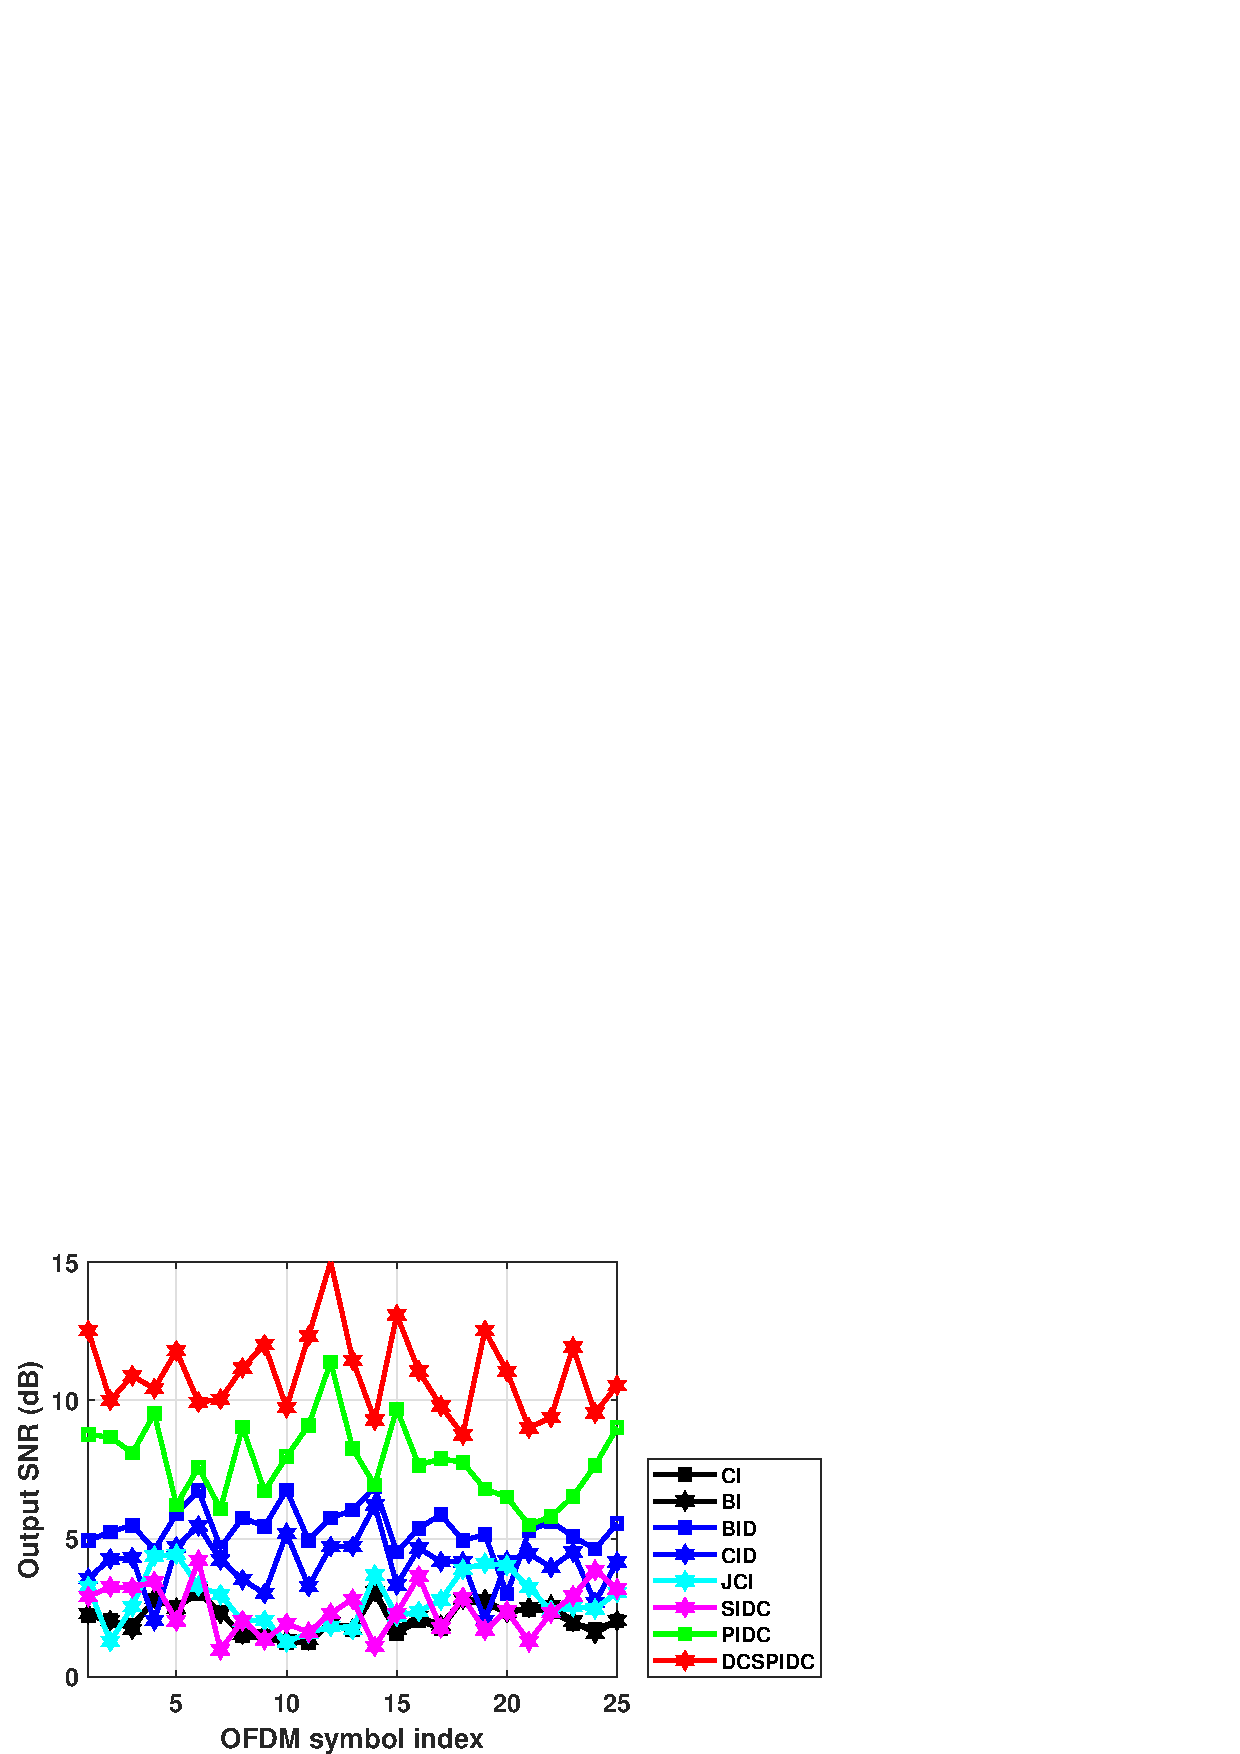
\includegraphics[width=8cm]{figs/Seatrial_OSNR.pdf}
%	\caption{Output SNR comparison in sea trial experiments.}\label{fig:Seatrial_OSNR}
%\end{figure}
\begin{figure*}[!htbp]
	\centering
	\subfloat[Conventional]
	{
		\label{fig:scatterplot_GAON}
		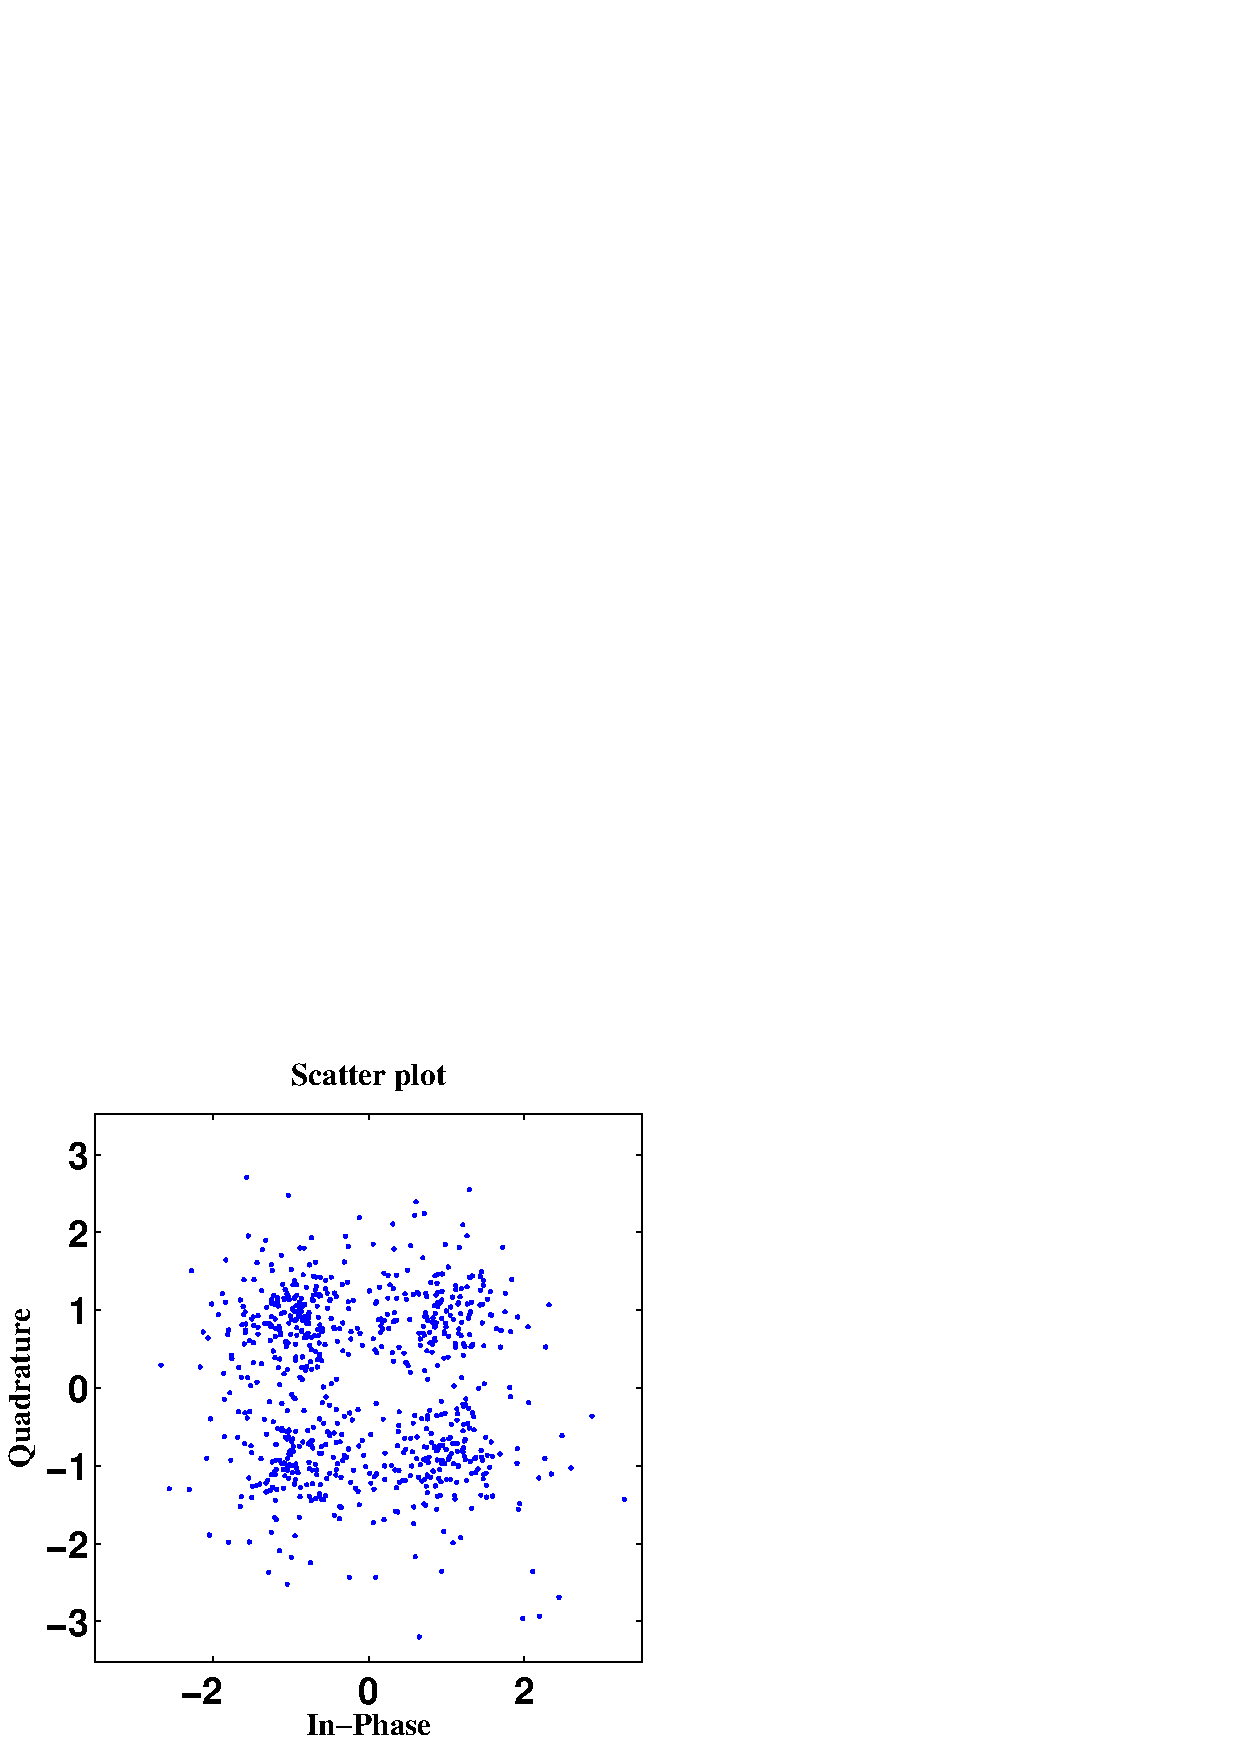
\includegraphics[width=0.24\textwidth]{figs/est_QPSK_GAON.pdf}
	}
	\subfloat[DSS-Net]
	{
		\label{fig:scatterplot_DSSNet}
		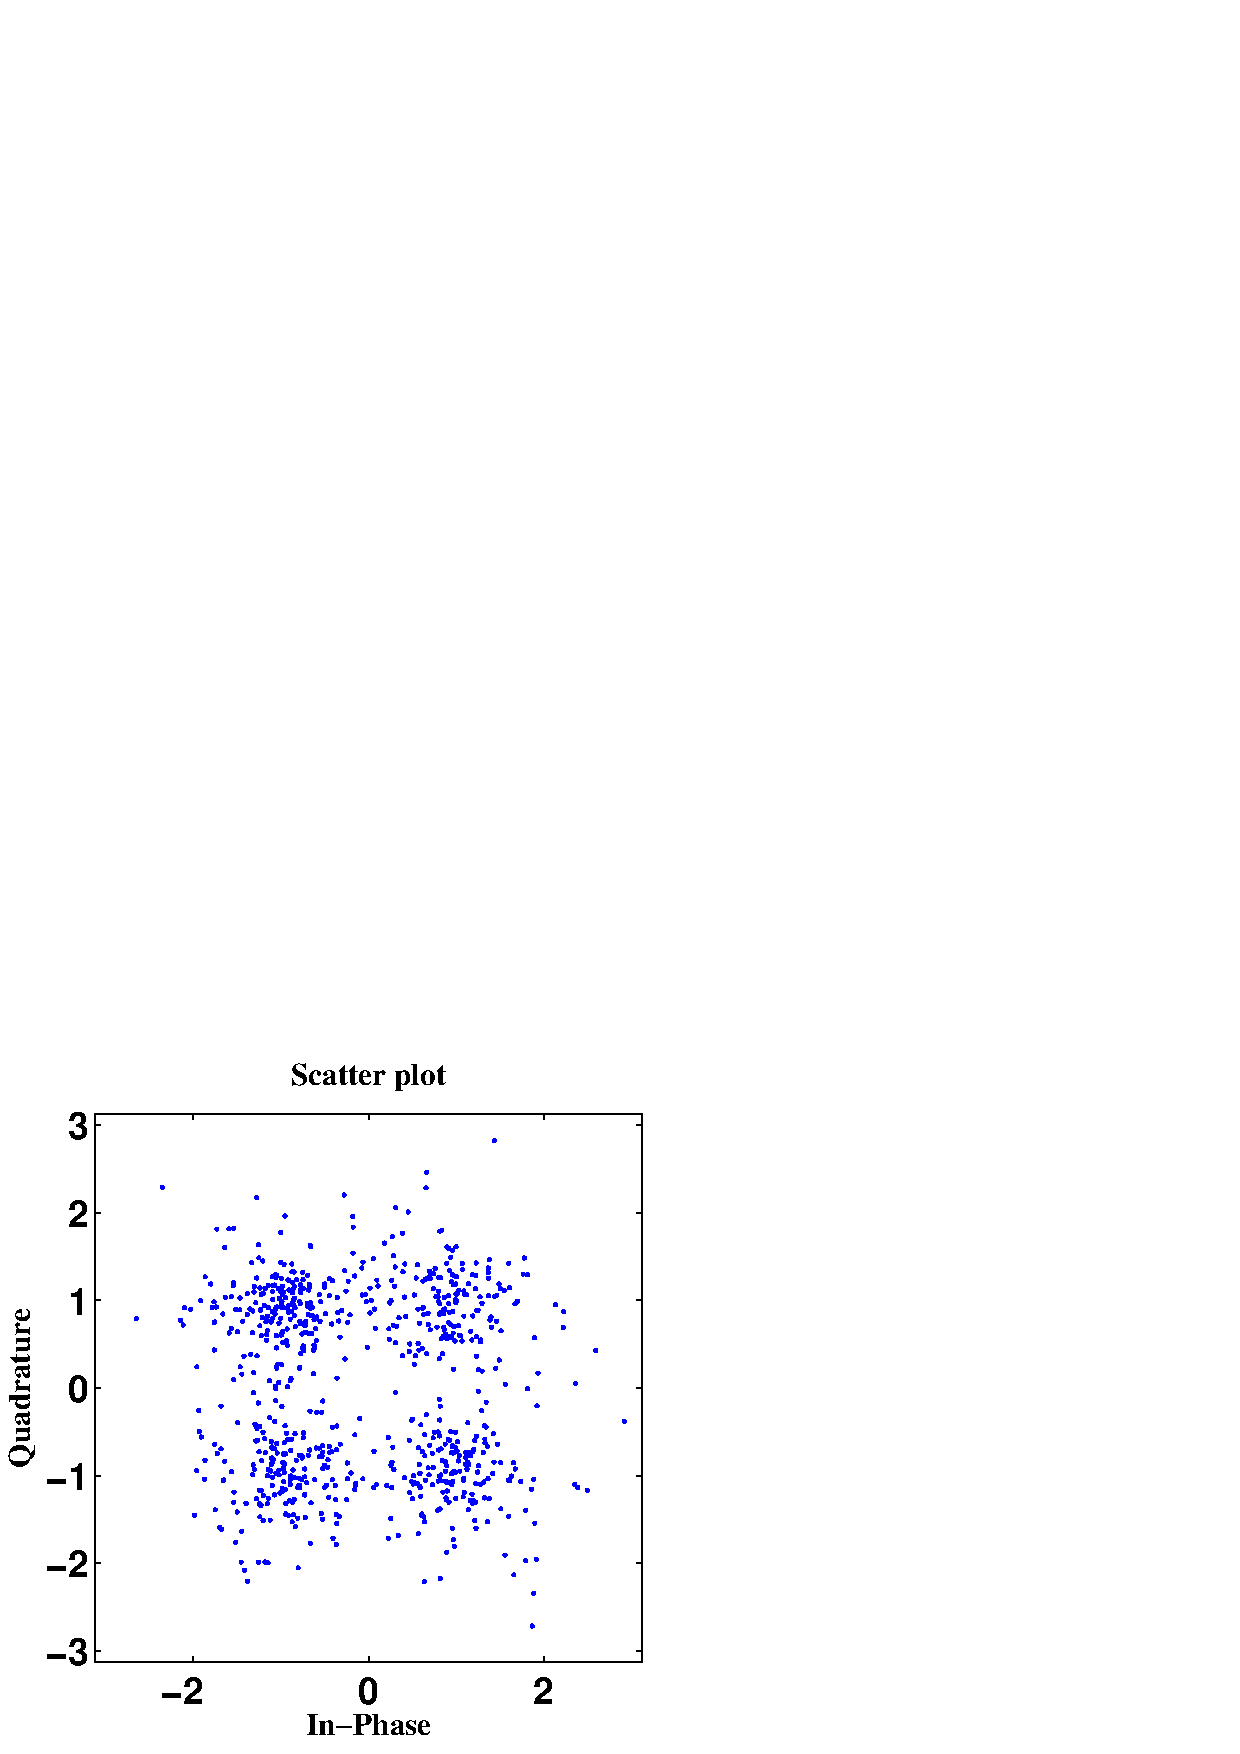
\includegraphics[width=0.24\textwidth]{figs/est_QPSK_GIAON.pdf}
	}
	\subfloat[w/o Attention]
{
		\label{fig:scatterplot_noatt}
		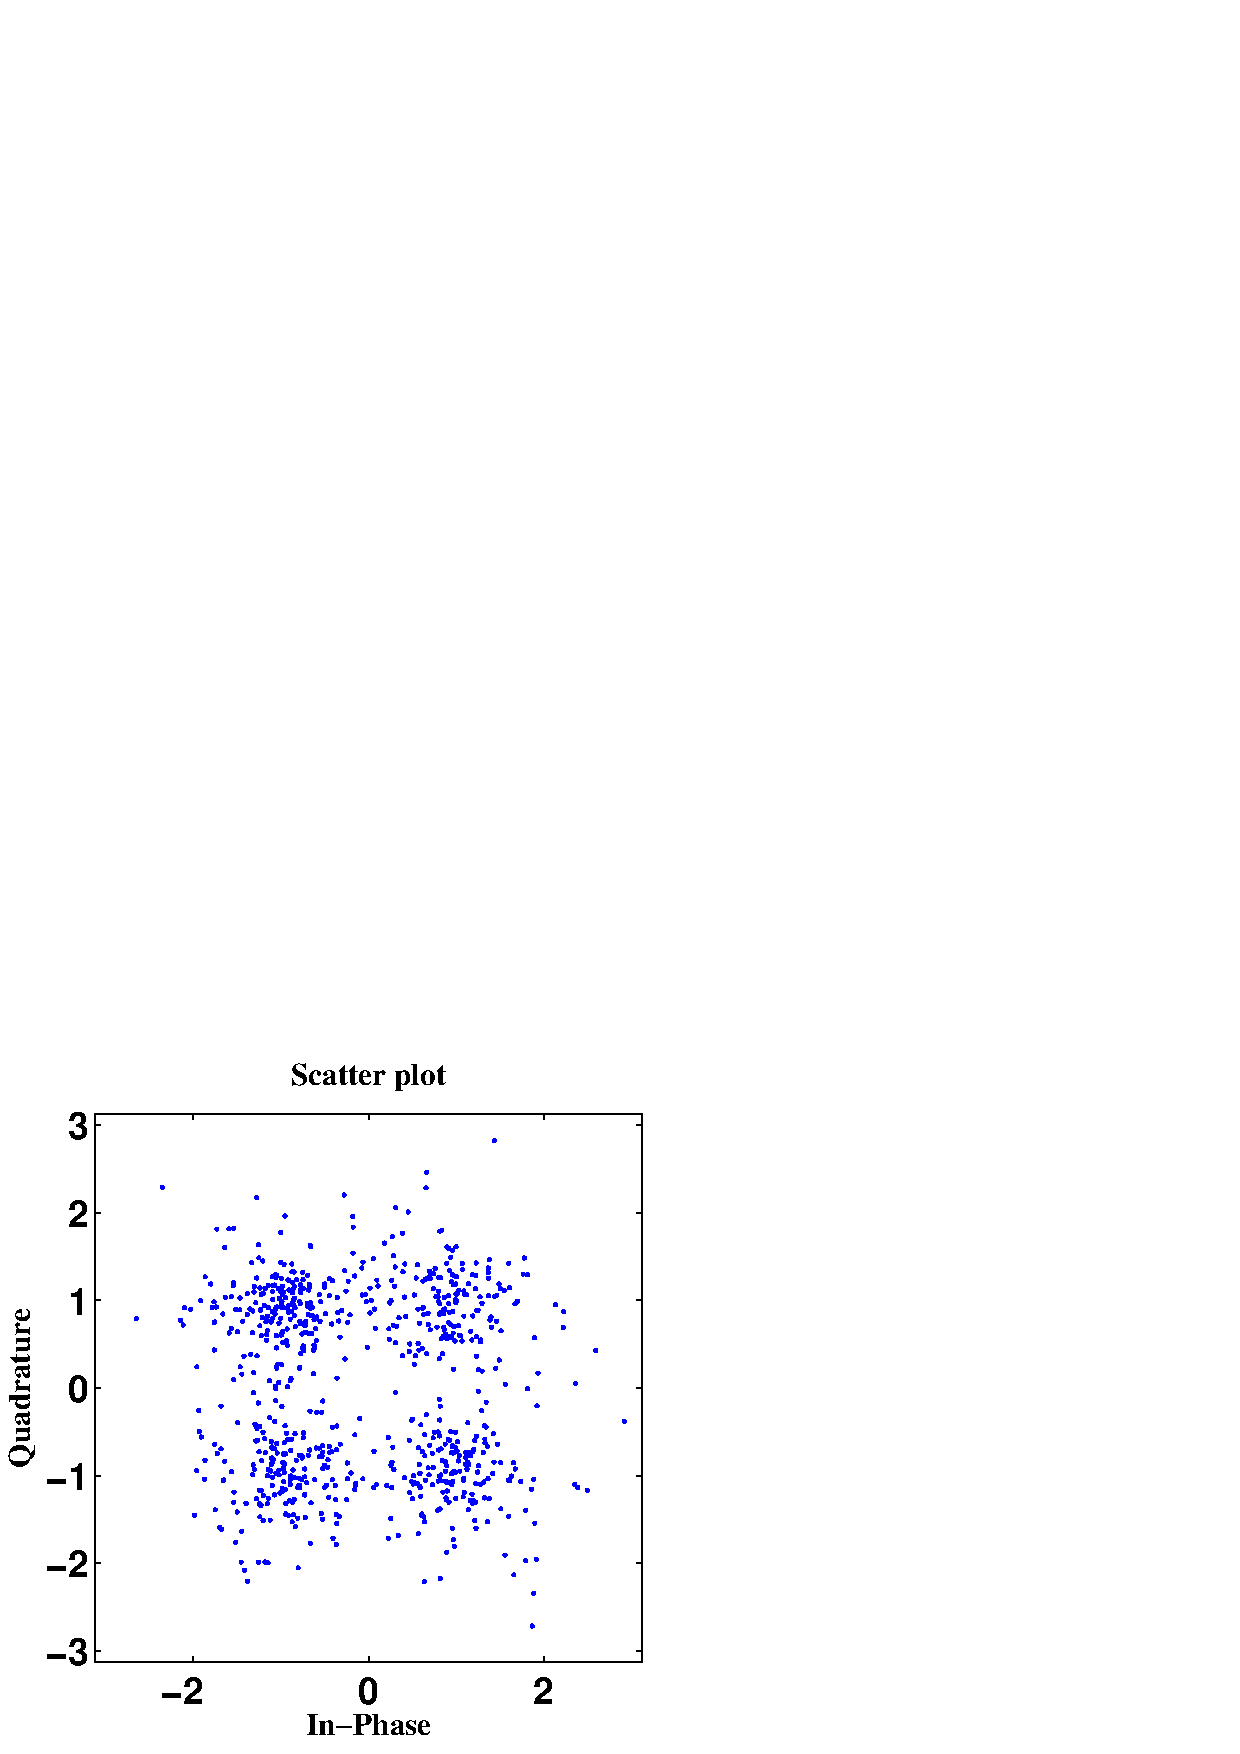
\includegraphics[width=0.24\textwidth]{figs/est_QPSK_GIAON.pdf}
}
	\subfloat[w/o Separation]
{
		\label{fig:scatterplot_nosep}
		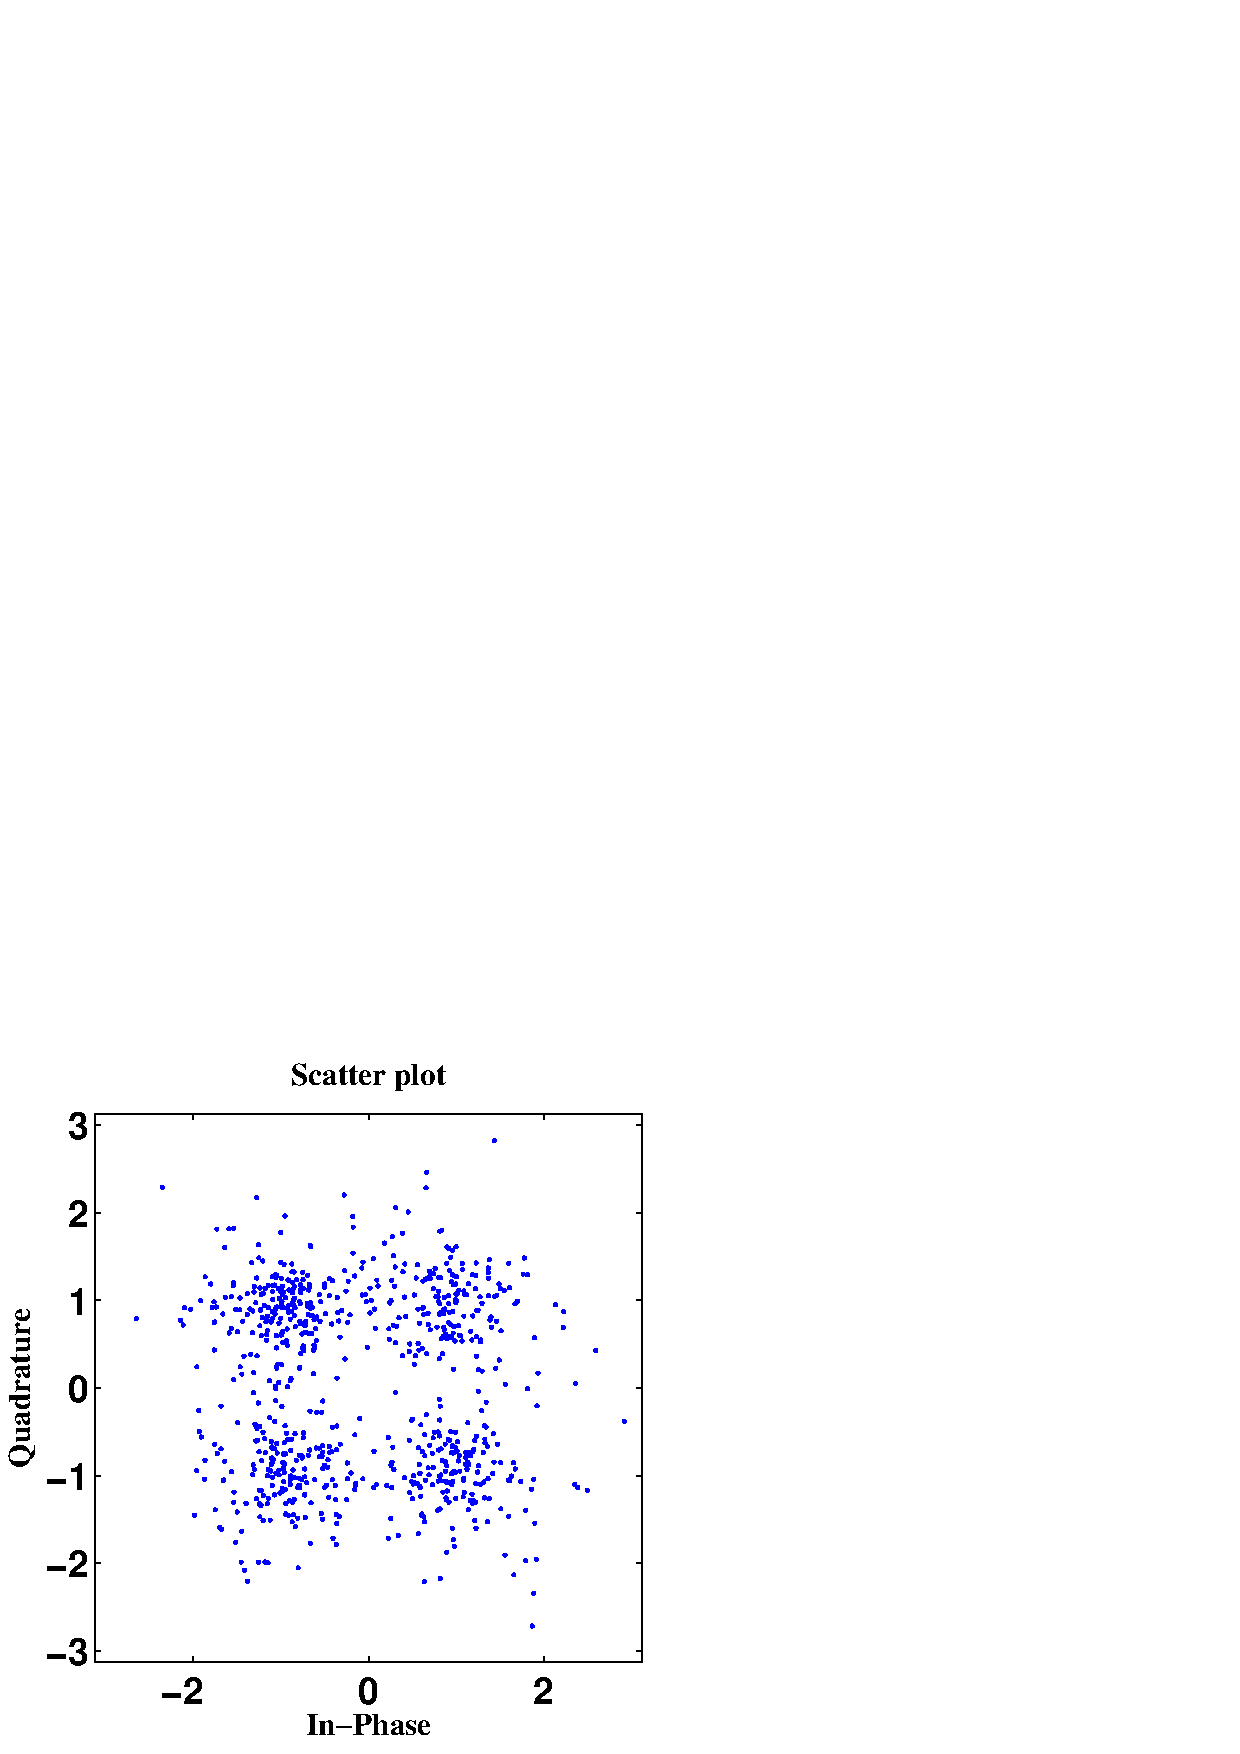
\includegraphics[width=0.24\textwidth]{figs/est_QPSK_GIAON.pdf}
}
	\caption{Output constellation diagram in the Wuyuan Bay experiment. (a) Conventional method. (b) DSS-Net. (c) DSS-Net w/o Attention. (d) DSS-Net w/o Separation.}
	\label{fig:scatterplot}
\end{figure*}

\subsection{Fuxian Lake Experiment}
\par A second sea trial was conducted in Fuxian Lake, Yunnan Province, China---the third deepest freshwater lake in China with a maximum depth of 155~m and exceptionally clear water (Secchi depth $>$12~m). Unlike the semi-enclosed shallow-water environment of Wuyuan Bay, Fuxian Lake provides a distinct propagation environment characterized by deep-water acoustics and minimal surface wave activity. The acoustic modem was deployed at depths of 5~m, 7~m, and 9~m, with a horizontal communication distance of approximately 484~m. The water depth at the experimental site was approximately 50~m.

\par Since ground-truth channel matrices are unavailable in real environments, we cannot compute the true NMSE. Instead, we report objective metrics that can be measured without ground truth. The \textit{power reduction} quantifies the power difference between input and output:
\begin{equation}
	\Delta P_{\text{dB}} = 10\log_{10}P_{\text{input}} - 10\log_{10}P_{\text{output}},
\end{equation}
where $P_{\text{input}}$ and $P_{\text{output}}$ denote the power of input (noisy) and output (denoised) channels, respectively. We emphasize that this metric represents power change, not necessarily noise removal---without ground truth, we cannot verify whether the removed power corresponds to noise or signal. Additionally, we report the static and dynamic component power ratios, which reflect the learned channel decomposition characteristics.

\par Table~\ref{tab:fuxian_results} summarizes the Fuxian Lake experimental results. Several physically meaningful observations emerge:
\begin{itemize}
	\item \textbf{Depth-dependent dynamic ratio}: As receiver depth increases from 5~m to 9~m, the dynamic component ratio increases from 23.8\% to 29.0\%. This is consistent with acoustic propagation physics: at greater depths, the receiver captures more surface-reflected paths, which are classified as dynamic components due to their time-varying nature.
	\item \textbf{Consistent power reduction}: DSS-Net consistently reduces power by 1.30--2.38~dB across all depths. While we cannot verify the removed component is purely noise without ground truth, the magnitude is consistent with the expected noise levels.
	\item \textbf{Component separation}: The static-to-dynamic power ratios (2.3--2.9:1) are consistent with the expected dominance of stable propagation paths in the relatively calm lake environment.
\end{itemize}

\begin{table}[htbp]
	\centering
	\caption{\textsc{Fuxian Lake Sea Trial Results.} Measured power changes and decomposition ratios of DSS-Net evaluated on real channel measurements at different receiver depths. Note: Without ground truth, true NMSE cannot be computed. Power reduction indicates energy removed by the network; static/dynamic ratios reflect the learned decomposition.}
	\label{tab:fuxian_results}
	\renewcommand{\arraystretch}{1.15}
	\setlength{\tabcolsep}{4pt}
	\small
	\begin{tabular}{>{\centering\arraybackslash}p{1.0cm} >{\centering\arraybackslash}p{1.3cm} >{\centering\arraybackslash}p{1.3cm} >{\centering\arraybackslash}p{1.3cm} >{\centering\arraybackslash}p{1.2cm} >{\centering\arraybackslash}p{1.2cm}}
		\toprule[1.5pt]
		\rowcolor{tableheader}
		\textbf{Depth} & \textbf{Input} & \textbf{Output} & \textbf{Power} & \textbf{Static} & \textbf{Dynamic} \\
		\rowcolor{tableheader}
		\textbf{(m)} & \textbf{(dB)} & \textbf{(dB)} & \textbf{Reduc.} & \textbf{Ratio} & \textbf{Ratio} \\
		\midrule[1pt]
		\rowcolor{tablerow1}
		5 & 2.35 & $-$0.03 & 2.38 & 69.3\% & 23.8\% \\
		\rowcolor{tablerow2}
		7 & 3.60 & 2.22 & 1.38 & 65.3\% & 24.6\% \\
		\rowcolor{tablerow1}
		9 & 2.72 & 1.42 & 1.30 & 52.8\% & 29.0\% \\
		\bottomrule[1.5pt]
	\end{tabular}
	\renewcommand{\arraystretch}{1.0}
\end{table}

\par The Fuxian Lake results, combined with the Wuyuan Bay experiments, demonstrate that DSS-Net generalizes effectively across diverse underwater environments---from shallow semi-enclosed bays with strong multipath to deep freshwater lakes with clearer propagation conditions. The consistent physical interpretability of the learned decomposition (increasing dynamic ratio with depth) provides confidence that DSS-Net captures meaningful acoustic propagation structures rather than arbitrary signal partitions.

% =========================================================================
\section{Conclusion}

This paper has proposed DSS-Net, a physics-inspired deep learning framework for UWA channel denoising through explicit dynamic-static decomposition. The key innovation lies in incorporating physical characteristics of UWA channels---static components from stable propagation paths with temporal consistency and sparsity, and dynamic components from time-varying sea surface reflections with low-rank structure---into both the network architecture and loss function design.

Simulation experiments on a large-scale ray-tracing dataset demonstrate that DSS-Net achieves $-25.27$~dB NMSE, representing a 4.86~dB improvement over baseline configurations. Ablation studies reveal the critical importance of physics-informed loss design, with hierarchical reconstruction weights, attention mechanisms, temporal constraints, and separation loss collectively contributing to the performance gains.

Two sea trial experiments were conducted to validate DSS-Net in real underwater environments. In the shallow semi-enclosed Wuyuan Bay, DSS-Net achieved 25.0\% BER improvement over conventional methods. In the deep freshwater Fuxian Lake, the learned channel decomposition exhibited physically consistent behavior: the dynamic component ratio increased with receiver depth (23.8\% at 5~m to 29.0\% at 9~m), reflecting the expected increase in surface-reflected paths. This depth-dependent decomposition pattern provides strong evidence that DSS-Net captures meaningful acoustic propagation structures rather than arbitrary signal partitions.

The proposed framework demonstrates that systematically incorporating domain knowledge---including channel decomposition structure, component-specific statistical properties, sparsity/low-rank priors, and temporal correlation characteristics---into deep learning can significantly outperform black-box approaches. Future work will extend DSS-Net to time-varying channel tracking and integrate it with adaptive modulation and coding schemes for complete UWA communication systems.

% =========================================================================
\appendices
\section{Proof of Proposition 1}

We prove the correlation bound under random scatterer distribution.

Let $\bm{H}_s$ be $k$-sparse in Delay-Doppler domain: $\|\bm{F}^H\bm{H}_s\|_0=k$. Let $\bm{H}_d=\bm{U}\bm{\Sigma}\bm{V}^H$ have rank $r$ with incoherent singular vectors satisfying $\|\bm{U}\|_{\infty}^2\leq\mu r/M$ and $\|\bm{V}\|_{\infty}^2\leq\mu r/N$ for incoherence parameter $\mu$ \cite{Candes2009Exact}.

The Frobenius inner product is
\begin{equation}
\langle\bm{H}_s,\bm{H}_d\rangle_F=\text{tr}(\bm{H}_s^H\bm{H}_d)=\sum_{mn}H_{s,mn}^*H_{d,mn}.
\end{equation}

By Cauchy-Schwarz:
\begin{equation}
|\langle\bm{H}_s,\bm{H}_d\rangle_F|\leq\|\bm{H}_s\|_F\|\bm{H}_d\|_F.
\end{equation}

Under random scatterer placement, angular-domain entries of $\bm{H}_s$ concentrate in $k$ bins with probability $(1-\delta)$. Incoherence of $\bm{H}_d$ ensures energy spreads uniformly. By concentration inequalities for random inner products \cite{Vershynin2018High}:
\begin{equation}
\mathbb{E}[|\langle\bm{H}_s,\bm{H}_d\rangle_F|]\lesssim\sqrt{kr}\|\bm{H}_s\|_F\|\bm{H}_d\|_F/\sqrt{MN}.
\end{equation}

Therefore:
\begin{equation}
\rho(\bm{H}_s,\bm{H}_d)=\frac{|\langle\bm{H}_s,\bm{H}_d\rangle_F|}{\|\bm{H}_s\|_F\|\bm{H}_d\|_F}\lesssim\sqrt{\frac{kr}{MN}}.
\end{equation}

This justifies our separation loss minimizing correlation.

\section{Nuclear Norm Gradient}

For $\bm{X}=\bm{U}\bm{\Sigma}\bm{V}^H$ with SVD, the nuclear norm is $\|\bm{X}\|_*=\text{tr}(\bm{\Sigma})$. By chain rule:
\begin{equation}
\nabla_{\bm{X}}\|\bm{X}\|_*=\nabla_{\bm{X}}\text{tr}((\bm{X}^H\bm{X})^{1/2})=\bm{U}\bm{V}^H.
\end{equation}

Detailed derivation follows \cite{Watson1992Characterization}. In practice, compute in float32 to avoid half-precision SVD failure.

% =========================================================================
\section*{Acknowledgments}
The authors thank the anonymous reviewers for constructive feedback.

% =========================================================================
\bibliographystyle{IEEEtran}
\bibliography{ref}

\end{document}